%%%%%%%%%%%%%%%%%%%%%%%%%%%%%%%%%%%%%%%%%%%%%%%%
% Doctoral thesis template for Tampere University of Technology
% 26.08.2014
% rev. 1.01
% 
%%%%%%%%%%%%%%%%%%%%%%%%%%%%%%%%%%%%%%%%%%%%%%%%
\documentclass[twoside,b5paper,openright]{memoir}
\usepackage[utf8]{inputenc}
\usepackage{tut_thesis}

%%%%%%%%%%%%%%%%%%%%%%%%%%% Select style of citations %%%%%%%%%%%%%%%%%

% author-year style
%\usepackage[sort]{natbib}

% superscripted numerical citations for e.g. chemistry theses
%\usepackage[sort,super]{natbib}


% numbered references style, replace 'sort&compress' with 'sort' 
% if you prefer [1],[2],[3] instead of [1-3] with multiple citations
%\usepackage[sort&compress,square,numbers]{natbib}

 \usepackage[natbibapa]{apacite}
% \usepackage[natbibapa]{apacite}
%%%%%%%%%%%%%%%%%%%%%%%%%%%%%%%%%%%%%%%%%%%%%%%%%%%%%%%%%%%%%%%%%%%%%%

% Since this a dissertation in hypermedia, we definitely want % to use hyperlinks here and there
\usepackage{hyperref}

% The following two packages are for inserting large tables in landscape mode. Not sure if such tables will be included in the final version of the dissertation.
\usepackage{pdflscape}
\usepackage{afterpage}

% Macro for controlling the TODO items include in different parts of the manuscript. One can e.g. exclude the items from the manuscript by commenting out the part that puts out the item. 
\newcommand{\todo}[1] {
\textbf{TODO}\textit{ #1}}

\newcommand{\guideline}[2] {
\textbf{Guideline #1:}\textit{ #2}}

%----------------------------------------------------------------------------------------
%	TITLE PAGE
%----------------------------------------------------------------------------------------

\newcommand*{\titleTH}{\begingroup % Create the command for including the title page in the document
\raggedleft % Right-align all text
\vspace*{\baselineskip} % Whitespace at the top of the page

{\Large Jukka Huhtamäki}\\[0.167\textheight] % Author name

{\LARGE\bfseries Dissertation}\\[\baselineskip] % First part of the title, if it is unimportant consider making the font size smaller to accentuate the main title

% Main title which draws the focus of the reader
{{\huge Ostinato Process Model for Visual Network Analytics}}\\[\baselineskip] 
% Tagline or further description
{\Large \textit{Experiments in Innovation Ecosystems}}\par 

% Whitespace between the title block and the publisher
\vfill 

\begin{figure}[htb]
% \centering

\includegraphics[width=8cm]{figure/tut-logo.pdf}
\label{fig:tut-logo}
\end{figure}

% {\large The Publisher \plogo}\par % Publisher and logo
\vspace*{3\baselineskip} % Whitespace at the bottom of the page
\endgroup}

\begin{document}
\frontmatter
\pagenumbering{gobble}
\titleTH
% Do not show page number on title page:
\pagenumbering{gobble}
% \thispagestyle{empty}
% \pagestyle{empty}
\clearpage
\pagenumbering{roman}
% \chapter{Tiivistelmä}

Innovaatiotoiminta ylittää enenevässä määrin organisaatioiden rajat ja siirtyy organisaatioiden ulkopuolelle ja väliin. Tähän innovaatiotoiminnan uuteen kontekstiin viitataan innovaatioekosysteemin käsitteellä. Avoin innovaatio, yhteiskehittely, käyttäjälähtöisyys, API- ja alustatalous ja liiketoimintaekosysteemit ovat muutoksen keskeisiä ajureita.  Innovaatioekosysteemit ovat kokonaisvaltaisia avoimia dynaamisia järjestelmiä, joilla on poliittinen, taloudellinen että teknologinen ulottuvuus. Lahjakkailla yksilöillä on aivan keskeinen rooli ekosysteemisessä innovaatiotoiminnassa. Liiketoimintaekosysteemeistä kumpuava innovaatioekosysteemien teoria määrittelee uuden viitekehyksen innovaatiotoiminnan analyysille ja tutkimukselle ja siten innovaatiotoiminnan mittaamiselle. 

Innovaatiotoiminnan mittaaminen ja visualisointi on haastavaa. Innovaatioekosysteemeissä haasteet lisääntyvät entisestään innovaatiotoiminnan kompleksisuuden takia. Jopa olennaisten toimijoiden ja sidosryhmien tunnistaminen on vaikeaa. Samalla on niin, että innovaatioekosysteemien järjestelmätason analyysi on avainasemassa kolmelle ryhmälle: innovaatioekosysteemien tutkijoille, politiikan ja innovaatiotoiminnan päätöksentekijöille sekä innovaatioekosysteemien toimijoille. Innovaatiotoimintaa edustavaa digitaalista dataa on saatavilla aikaisempaa enemmän ja periaatteelliset mahdollisuudet järjestelmätason analyysiin ovat siten parantuneet. Tässä väitöskirjatyössä tavoitteena onkin edistää mahdollisuuksia digitaalisen datan soveltamiseen innovaatioekosystemien järjestelmätason analyysin toteuttamisessa. 

Tässä toimintadesigntutkimuksen otteella toteutetussa väitöskirjassa kehitetään tapoja tarkastella innovaatioekosysteemien rakenteellisia ominaisuuksia järjestelmätasolla visuaalisen verkostoanalytiikan keinoin. Keskeinen lähtökohta tutkimustyölle on havainto siitä, että  toimijoiden väliset kytkökset ovat avainasemassa innovaatioekosysteemeissä. Verkostoanalyysi tarjoaa luontevan keinon innovaatioekosysteemien rakenteellisen analyysin toteuttamiseen. Verkostoanalyysi antaa innovaatioekosysteemien tutkijoille ja toimijoille mahdollisuuden tehdä havaintoja innovaatioekosysteemien rakenteesta ja toimijoiden rakenteellisista rooleista. Tutkimme tässä työssä joukon erilaisia innovaatioekosysteemejä alustapohjaisesta kansalliseen ja kansainväliseen sekä kasvua tukevaan ohjelmatoimintaan tavoitteenamme tunnistaa tapoja innovaatioekosysteemien mallintamiseen ja analysointiin verkostoina. Työn päätavoite on kehittää prosessimalli innovaatioekosysteemien rakenteelliseen tarkasteluun visuaalisen analytiikan keinoin  datalähtöisen laskennallisen analytiikan tuella. 

Osoitamme tässä työssä että verkostoanalyysi tuo lisäarvoa innovaatioekosysteemien verkostorakenteen kartoittamiseen ja tutkimiseen. Ehdotetussa lähestymistavassa innovaatioekosysteemien toimijoita ja heidän vuorovaikutustaan edustavaa transaktionaalista mikrodataa kerätään moninaisista digitaalisista lähteistä. Innovaatioekosysteemin toimijat esitetään verkoston solmuina, jotka kytketään toisiinsa transaktioiden ja muiden yhteyksien perusteella. Sijoitukset, yrityshankinnat ja erilaiset sopimukset sekä neuvonantajana, perustajana tai keskeisenä työntekijänä toimiminen ovat esimerkkejä yhteyksistä. Verkostoanalyysin tunnusluvut mahdollistavat erilaisten toimija- ja järjestelmätason ominaisuuksien esittämisen lukuarvoina. Verkostot visualisoidaan eksploratiivisen analyysin ja tulosten raportoimisen tueksi vuorovaikutteisilla välineillä, jotka mahdollistavat joustavan liikkumisen sekä yksityiskohtia että kokonaisuuksia valottavien näkymien välillä.

Tämä väitöskirjatutkimus edistää innovaatioekosysteemien datalähtöisen visuaalisen verkostoanalyysin teoriaa ja käytäntöä useilla tavoilla. Väitöskirjatutkimuksen keskeinen tulos on Ostinato-malli, joka mahdollistaa iteratiivisen, käyttäjäkeskeisen tavan toteuttaa automatisoituja datalähtöisen visuaalisen verkostoanalyysin prosesseja. Ostinato-malli jakaa innovaatioekosysteemin analyysiprosessissa kahteen vaiheeseen, 1) datan kerääminen ja jalostaminen sekä 2) verkoston luominen ja analyysi. Datan kerääminen ja jalostaminen toteutetaan neljällä askeleella: entiteetti-indeksin luominen, webin ja ohjelmointirajapintojen ryömiminen, datan raapiminen, ja datan koostaminen. Verkoston luominen ja analyysi muodostuu seitsemästä askeleesta: entiteettien valinta, solmujen ja yhteyksien luominen, tunnuslukujen laskenta, solmujen ja yhteyksien suodattaminen, entiteetti-indeksi täsmentäminen ja visuaalisten ominaisuuksien määrittely. Vuorottelu eksploraation ja automatisoinnin välillä leikkaa läpi prosessin vaiheiden. 

Ostinato-mallin ohella tässä väitöskirjassa määritellään joukko ohjenuoria innovaatioekosysteemien verkostomallinnuksen ja visuaalisen verkostoanalyysityön tueksi. Väitöskirja antaa myös panoksensa innovaatioekosysteemien empiiriseen tietämykseen mallintamalla joukon eri abstraktio- ja kompleksisuustasoja edustavia innovaatioekosysteemejä. Tutkimuksen kohteena olleiden innovaatioekosysteemien tutkijat, politiikan päätöksentekijät, orkestroijat ja muut toimijat ovat omaksuneet esitetyn lähestymistavan. Lähestymistavan kattava hyödyntäminen organisaatiorajat ylittävien innovaatiotoimien tutkimisessa, tukemisessa ja orkestroinnissa edellyttää lisää tutkimusta ja tuotekehitystä.
\chapter{Tiivistelmä}

\textbf{Mitä?} Innovaatiotoiminta siirtyy enenevässä määrin organisaatioiden ulkopuolelle ja organisaatioiden väliin. Avoin innovaatio, yhteiskehittely, käyttäjälähtöisyys, API- ja alustatalous ja liiketoimintaekosysteemit ovat muutoksen keskeisiä ajureita. Liiketoimintaekosysteemeistä kumpuava innovaatioekosysteemien teoria määrittelee uuden viitekehyksen innovaatiotoiminnan analyysille ja tutkimukselle ja siten innovaatioekosysteemien mittaamiselle. Innovaatioekosysteemit ovat kononaisvaltaisia organisaatioiden rajat ylittäviä, poliittisia, taloudellisia ja teknologisia innovaatiojärjestelmiä, jotka tarjoavat viljavat puitteet liiketoiminnan kasvun kiihdyttämiselle ja jatkuvuudelle kestävällä tavalla.

Tässä toimintatutkimuksen ja design-tutkimuksen otteilla toteutetussa väitöskirjassa kehitetään kokonaisvaltainen prosessimalli innovaatioekosysteemien datalähtöisen laskennallisen visuaalisen rakenteellisen analyysin tueksi. Verkostoanalyysi tarjoaa luontevan keinon innovaatioekosysteemien rakenteellisen analyysin toteuttamiseen. Datalähtöisyys viittaa tässä työssä kykyyn kerätä dataa erilaisista digitaalisista lähteistä analyysin lähteeksi ja analysoida dataa automatisoidusti innovaatioekosysteemien tutkimuksen tueksi.

\textbf{Miksi?} Innovaatioekosysteemien järjestemätason visuaalinen rakenneanalyysi tukee kolmea keskeistä innovaatioekosysteemeihin liittyvää toimintaa: innovaatioekosysteemien analytiikkaa päätöksenteon tukena, innovaatioekosysteemien akateemista tutkimusta sekä sekä innovaatioekosysteemien johtamista orkestroinnin periaatteiden mukaisesti. 

\textbf{Miten?} Innovaatioekosysteemin toimijat esitetään solmuina, jotka kytketään toisiinsa toimijoiden välisten yhteyksien ja transaktioiden perusteella. Verkostot visualisoidaan eksploratiivisen analyysin ja tulosten raportoimisen tueksi. Verkostoanalyysin tunnusluvut mahdollistavat erilaisten toimija- ja järjestelmätason ominaisuuksien esittämisen tunnuslukuina. Näitä tunnuslukuja voidaan käyttää sekä innovaatioekosysteemien määrällisessä tutkimuksessa että visualisointien ominaisuuksien määrittelemisessä

\textbf{Tulokset ja kontribuutio?} Väitöskirjatutkimuksen keskeinen tulos on Ostinato-malli. Ostinato-malli jakaa innovaatioekosysteemin analyysiprosessissa kahteen vaiheeseen, 1) datan kerääminen ja jalostaminen sekä 2) verkoston luominen ja analyysi. Datan kerääminen ja jalostaminen toteutetaan neljässä vaiheessa: entiteetti-indeksin luominen, Webin ja ohjelmointirajapintojen ryömiminen, datan raapiminen, ja datan koostaminen. Verkoston luominen ja analyysi muodostuu seitsemästä vaiheesta: entiteettien valinta, solmujen ja yhteyksien luominen, tunnuslukujen laskenta, solmujen ja yhteyksien suodattaminen, entiteetti-indeksi täsmentäminen ja visuaalisten ominaisuuksien määrittely. 

Ostinato-mallin ohella tässä väitöskirjassa määritellään joukko ohjenuoria innovaatioekosysteemien verkostomallinnuksen ja visuaalisen verkostoanalyysityön tueksi. Väitöskirja antaa myös oman panoksensa innovaatioekosysteemien empiiriseen tietämykseen mallintamalla joukon eri abstraktiotasolle sijoittuvia innovaatioekosysteemejä.

\chapter{Abstract}
\label{chapter:abstract}

\textbf{What?} 
% Innovation is imperative in sustaining and developing any business. Moreover, successful and sustainable businesses are key in developing thriving programs, regions, countries and continents. 
More often than ever before, innovation is taking place in between the formal organizational structures. It is taking place in innovation ecosystems. Open innovation, co-creation, user driven innovation, API and platform economy and business ecosystems are key drivers of the transformation. Innovation ecosystem theory sets a new framework for analyzing and investigating and therefore measuring the ecosystems. Innovation ecosystems are open dynamic systems that cross the organizational and geographical boundaries and include financial, technological and political dimensions. Innovation ecosystems introduce new means to develop new businesses and industries in a sustainable manner. 

\textbf{Why?} Innovation ecosystems present a natural habitat for exercising data-driven visual network analytics. Multiple sources of data with varying quality exists for tracking down activities of innovation ecosystem actors representing different organizations. Moreover, there is an imperative need for system-level view for the ecosystems. Innovation ecosystems are rather orchestrated than managed, therefore groups of people have to come together to form shared vision on a future that they want to pursue together.  

Addressing innovation ecosystems as networks allows scholars and practitioners to study their complexity, providing a means for mapping, monitoring and managing the ecosystem components. To do this, we take a data-driven network analysis approach to study innovation ecosystems in regional, metropolitan, national and international level as well as e.g. in the context of programmatic activities supporting innovation and growth. We Action Design Research approach that is based on iteration through construction of network visualizations as artifacts. We use a number of different datasets in these studies, including social media, socially constructed data available online, and proprietary sets of data represented as spreadsheets and other formats.

\textbf{How?}
Network analysis is valuable method for investigating and mapping the social structure driving all kinds of phenomena and sharing the findings with others. The interactive visual analytics approach transforms data into views that allow the visual exploration of the structure and evolution of networks represented by data, therefore increasing the transparency of the roles of innovation ecosystems actors and the patterns emerging from their individual activities. 

\textbf{Results and contribution} This dissertation makes several contributions in pushing forward the art and science of data-driven visual network analytics of innovation ecosystems. Most importantly, the dissertation presents the Ostinato Model, an iterative, user-centric, process-automated model for data-driven visual network analytics. The Ostinato Model simultaneously supports the automation of the process and enables interactive and transparent exploration. The model has two phases, Data Collection and Refinement and Network Creation and Analysis. The Data Collection and Refinement phase is further divided into Entity Index Creation, Web/API Crawling, Scraping, and Data Aggregation. The Network Construction and Analysis phase is composed of Filtering in Entities, Node and Edge Creation, Metrics Calculation, Node and Edge Filtering, Entity Index Refinement, Layout Processing and Visual Properties Configuration. A cycle of exploration and automation characterizes the model and is embedded in each phase.

In addition to the Ostinato Model, this dissertation contributes to the empirical body of knowledge on innovation ecosystems with a set of design guidelines for modeling and visualizing innovation ecosystems as networks. Finally, the dissertation contributes with a set of empirical investigations of innovation ecosystems of different levels of abstraction and complexity from platform, industry, program, national to international. Policy makers, orchestrators and other stakeholder of the innovation ecosystem under investigation have subscribed to the approach presented in this dissertation. More research and development of supporting processes and tools are needed to take full advantage of the presented approach in facilitating and orchestrating inter-organizational innovation activities. 
% Bring back to the final version after pre-examination
% \chapter{Preface}  
\label{chapter:Preface}

This study was carried out at Intelligent Information Systems Laboratory (IISLab) at Tampere University of Technology (TUT). IISLab is part of the Department of Mathematics. IISLab was previously know as Hypermedia Laboratory. ...

I would like to express my sincere gratitude to ...

\emph{This is going to be a long story. Trying to keep it under two pages, though. A draft is in process in Evernote.}

%disable microtype features during table of contents
\microtypesetup{protrusion=false}
\cleardoublepage
\tableofcontents* %starred version prevents 'Contents' from being listed
\microtypesetup{protrusion=true}

% include your chapters below
% Bring back and extend nomenclature if it turns out that
% it would be important to show off with graph theoretical and 
% mathematical notation  
% %Feel free to replace the manual listing below with something else, e.g. using the nomencl or glossaries package


\chapter{Nomenclature}
\label{chapter:nomencl}

\emph{This could a place to show off some graph-related mathematical notations. Removing the chapter is a more likely option, however.}

In 2006, Jyri Engeström and Petteri Koponen founded Jaiku, a social media before social media. Next year, Google acquired Jaiku and Engeström and Koponen moved forward, first to work at Google and then to other startup and business ventures. Currently, Koponen is one of the founders of Lifeline Ventures, a venture capital investment company. Lifeline Venture's portfolio includes Supercell, a game-development company that, in 2015, is one of the keystone companies of the Finnish Innovation Ecosystem. In 2014, Supercell CEO Ilkka Paananen and Petteri Koponen after a Japanese giant acquired part of Supercell, Supercell CEO and Koponen together with the Timo Ahopelto, also a partner at Lifeline Ventures, joined to start up a new fund\footnote{Supercell-miljonäärit ryhtyvät sijoittajiksi, \url{http://www.hs.fi/talous/a1398050554829}} for providing seed level funding to Finnish Startups and growth companies.

After receiving information on just a few of these kinds of storylines or chains of action, as humans with limited cognition, we begin to loose the big picture, the system-level view. Is there a way to represent these stories in data and to quantify them for analysis and visualization?

The thesis of this dissertation is that visual network analytics is an imperative approach in allowing the exploration of innovation ecosystem structure. A graph is composed of nodes and edges connecting the nodes.

… 

% DO NOT START WRITING A SECTION ON GRAPH AND NETWORK BASICS BEFORE SOMEONE ACTUALLY INSISTS ON DOING SO! :)

% \textbf{Latin alphabet}
% \begin{longtable}[l]{p{2cm} p{12cm} }
% $^{i}a^{x}_{P_{\,i}^j}$ & $x$ axis component of $^i\mathbf{a}_{P_{\,i}^j}$    \\
% $\{B\}$ & body coordinate frame  \\
% $\mathbf{\dot{x}}^{\,ref}$ & end-effector velocity reference  \\
% $Y(s)$ & position output \\
% \end{longtable}

% \textbf{Greek alphabet}
% \begin{longtable}[l]{p{2cm} p{12cm}}
% $_G\,\boldsymbol{\alpha}_B$ & angular acceleration of $\{B\}$ with respect to $\{G\}$ \\
% $^{i}\boldsymbol{\alpha}_i$ & angular velocity of $\{B_i\}$ with respect to $\{I\}$ expressed in $\{B_i\}$  \\
% $\boldsymbol{\mu}_m$ & additive magnetometer measurement noise \\
% $^i_j\,\boldsymbol{\dot{\omega}}_{k}$ & angular acceleration of $\{B_{k}\}$ relative to $\{B_j\}$ expressed in $\{B_i\}$  \\
% \end{longtable}

\chapter{List of Publications}

\begin{midsloppypar}

This dissertation is a compilation of seven (7) publications, of which four (2) are journal articles, four (4) appear in conference proceedings and one (1) is published as a chapter of a peer-reviewed scientific book.

In this section, we will describe the role of the author of this dissertation in each of the publications and add further information about them. Finnish Publication Forum\footnote{Finnish Publication Forum, \url{http://www.tsv.fi/julkaisufoorumi/english.php}} ratings are used to roughly indicate the quality of the publication channels. (Level 3 is the highest.)

\begin{enumerate}[label=\textbf{Publication \Roman*},align=left]

  \item Jukka Huhtamäki, Ville Luotonen, Ville Kairamo, Kaisa Still, Martha G. Russell 
  (2013)
  "Process for Measuring and Visualizing an Open Innovation Platform: Case Demola,"
  \emph{Academic MindTrek 2013, Tampere, Finland}.
  Publication Forum level 1.
  \label{pub:demola}

  \item Rahul C. Basole, Martha G. Russel, Jukka Huhtamäki, Neil Rubens
  (2012)
  "Understanding Mobile Ecosystem Dynamics: A Data-Driven Approach,"
  \emph{International Conference on Mobile Business (ICMB)}.
  Publication Forum level 1.
  \label{pub:mobileecosystem}

  \item Jukka Huhtamäki, Kaisa Still, Minna Isomursu, Martha G. Russell and Neil Rubens
  (2012)
  "Networks of Growth: The Case of Young Innovative Companies in Finland," 
  \emph{The 7th European Conference on Entrepreneurship and Innovation (ECIE 2012, Santarém, Portugal}.
  Publication Forum level 0.
  \label{pub:tekesyic}

  \item Jukka Huhtamäki, Martha G. Russell, Kaisa Still, Neil Rubens
  (2013)
  "A Network-Centric Snapshot of Value Co-Creation in Finnish Innovation Financing," 
  \emph{Value Co-Creation: Best of TIM Review}.
  Publication Forum level 0; TIM Review was promoted to Publication Forum level 1 in 2015.
  \label{pub:finland}

  \item Kaisa Still, Jukka Huhtamäki, Martha G. Russell, Rahul C. Basole, Jaakko Salonen, Neil Rubens
  (2013)
  "Networks of innovation relationships: multiscopic views on Finland,"
  \emph{International Society for Professional Innovation Management (ISPIM) 2013, Helsinki}.
  Publication Forum level 0.
  \label{pub:multiscopicfinland}

  \item Kaisa Still, Jukka Huhtamäki, Martha G. Russell, Neil Rubens
  (2014)
  "Insights for orchestrating innovation ecosystems: the case of EIT ICT Labs and data-driven network visualisations,"
  \emph{International Journal of Technology Management}.
  Publication Forum level 1. 
  \label{pub:eitictlabs}
  
  \item Jukka Huhtamäki, Martha G. Russell, Neil Rubens, Kaisa Still 
  (2015) 	
  "Ostinato: The exploration-automation cycle of user-centric, process-automated data-driven visual network analytics," in Sorin Adam Matei,
Elisa Bertino, Russell, Martha G. (Eds.) \emph{Transparency in Social Media: Tools, Methods and Algorithms for Mediating Online Interactions},
  Springer. Publication Forum level 2.
  \label{pub:ostinato}
  
\end{enumerate}

\section{Authors role and quality of publication channels}

The series of investigations that form the first part of results for this dissertation are conducted by the Innovation Ecosystems Network (IEN) team. The majority of the work took place under Tekes innovation research projects SINDI (2010-2012), REINO (2012-2015) and SPEED (2014-2016). The author of this dissertation is one of the co-founders of IEN. Martha G. Russell, mediaX at Stanford University, leads the IEN team that include Kaisa Still, VTT Technical Research Centre of Finland  Ltd; Neil Rubens, University of Electro-Communications, Tokyo; Rahul C. Basole, Georgia Tech and Camilla Yu, VXPLO Innovation Lab.

The author of the dissertation has led the design, development and operation of the data-driven visual analytics process in each of the investigations. Moreover, the author has written the majority of the manuscript for \ref{pub:demola}, \ref{pub:tekesyic}, \ref{pub:finland} as well as \ref{pub:ostinato}. In others, the author has made significant contributions to research design, manuscripts, analysis, discussion, and research project management.

\ref{pub:demola} was presented by the author of this dissertation at Academic MindTrek in Tampere, Finland. Academic MindTrek (MindTrek Conference in Publication Forum) is placed in Publication Forum level 1.

\ref{pub:tekesyic} was presented in ECIE 2012 by the author of this dissertation. ECIE is placed in Publication Forum level 0.

\ref{pub:mobileecosystem} received the Best Paper Award in International Conference on Mobile Business (ICMB). ICMB is in Publication Forum level 1.

\ref{pub:finland} was originally presented by the author of this dissertation at the 10th annual EBRF conference in Nokia, Finland. The article was first invited to Technology Innovation Management Review. Later, the article was selected to be included into Best of TIM Review book. In 2015, TIM Review was promoted to Publication Forum level 1.

\ref{pub:multiscopicfinland} was co-presented by Kaisa Still and the author of this dissertation at ISPIM in Helsinki. While ISPIM is placed in Publication Forum level 0, it is considered a key yearly meeting in innovation research domain.

\ref{pub:eitictlabs} was invited to be published in a Special Issue of International Journal of Technology Management (IJTM) on Business and Network Models for Innovation. IJTM is placed in Publication Forum level 1.

\ref{pub:ostinato} was selected to be included in the second volume of Roles, Trust, and Reputation in Social Media Knowledge Markets, a book published by Springer. As a book publisher, Springer is placed in Publication Forum level 2.

\end{midsloppypar}

\mainmatter

\chapter{Introduction}
\label{chapter:intro}

Innovation--what is it and why it is important? Innovation refers to the ability to create and capture economic value from invention \citep{Hagel2005TheSpecialization}. Innovation is key driver of any sustainable business and, indeed, society. Innovation has become an imperative for business, academic and governmental organizations in response to environmental and technology-driven changes \citep{Drucker2015InnovationPrinciples,VandeVen1986CentralInnovation,Gupta2007InnovationAnalysis,Schumpeter1942CapitalismDemocracy}. \cite{Carlson2006}, among others, underline the imperative role of innovation: ``Nothing is more important to business success than innovation.'' Over the past century, conceptual approaches for understanding and accelerating innovation have evolved. 

What are innovation ecosystems and why are they relevant in 2016? More often than ever before, innovation is taking place outside the boundaries of and in between individual organizations. Moreover, customers now have an active role in innovation, i.e. in value co-creation. Through open innovation and value co-creation, several steps have been taken from manufacturing-driven, technology-push view \citep{Schumpeter1934TheCycle,Schumpeter1942CapitalismDemocracy,Schumpeter1950TheSocialism} to that of the ecosystemic view both to business and innovation \citep{Russell2011TransformingOrchestration,Moore1993PredatorsCompetition,Jarvi2013}. \cite{Autio2013InnovationManagement} define innovation ecosystem as ``a network of interconnected organizations, organized around a focal firm or a platform, and incorporating both production and use side participants, and focusing on the development of new value through innovation.'' \cite{Russell2011TransformingOrchestration} take an even broader view to define innovation ecosystem as an ``inter-organizational, political, economic, environmental and technological systems of innovation through which a milieu conducive to business growth is catalyzed, sustained and supported.'' In system level, individual relationships take the shape of a network ``through which information and talent flow through systems of sustained value co-creation'' \citep{Russell2015RelationalEcosystems}.

Key influence in the adoption of the ecosystem concept in the context of innovation is the concept of business ecosystem that \cite{Moore1993PredatorsCompetition} introduced. Ecosystem is used in this context both as a metaphor \citep[e.g.][]{Hwang2012}, a strategy artifact \citep{Moore1993PredatorsCompetition}, as well as to refer to system-level analysis \citep[cf.][]{Pentland2015}. Innovation ecosystems are orchestrated rather than controlled or managed \citep{Russell2011TransformingOrchestration, Ritala2009, Ritala2013}. When collective gains are sought at the network level, change agents seek to facilitate the emergence of networks, orchestrate existing networks and manage their growth \citep{Russell2011TransformingOrchestration}. To manage innovation ecosystems as well as to facilitate their emergence, the process of network orchestration is encouraged \citep{Russell2015RelationalEcosystems}.

Why visual network analysis is valuable in exploring innovation ecosystems? Measuring and visualizing innovation is hard. This is particularly true for innovation ecosystems where innovation activities take very complex forms and even the identification of relevant actors and stakeholders is challenging. At the same time, system-level analysis of innovation ecosystems is imperative for three groups: innovation ecosystem scholars, policy and decision makers, and innovation ecosystem actors. Moreover, new sources of digital data on innovation activities have become available. This dissertation seeks to bridge the gap between opportunities provided by the digital data available and the desire to investigate innovation ecosystems in system level.

\begin{quote}
``Use a picture. It's worth a thousand words.'' -Arthur Brisbaine \citep{Bendoly2016FitAnalytics}
\end{quote}

\begin{quote}
``...few people will appreciate the music if I just show them the notes. Most of us need to listen to the music to understand how beautiful it is. But often that’s how we present statistics; we just show the notes we don’t play the music.'' - Hans Rosling 
\end{quote}

In this dissertation, innovation ecosystems are investigated with a visual network analytics approach. From the beginning of social network analysis and its precursor, sociometry, visualization has been a key part of the analysis process, cf. \cite{Moreno1953}:
\begin{quote}
``We have first to visualize [...] A process of charting has been devised by the sociometrists, the sociogram, which is more than merely a method of presentation. It is first of all a method of exploration. It makes possible the exploration of sociometric facts. The proper placement of every individual and of all interrelations of individuals can be shown on a sociogram. It is at present the only available scheme which makes structural analysis of a community possible.''\end{quote}

Explorative visual analysis of networks and therefore ecosystems allows holistic investigations as well as sharing the findings to others \citep{Freeman2000VisualizingNetworks}. The challenges and opportunities of visualization in general and  visual network analytics specifically have received little attention in innovation ecosystem research. \cite{Basole2014} states that while research on challenges and opportunities of visualization in corporate settings exists \citep{Lam2012,Sedlmair2011}, ``researchers haven’t focused on visual business ecosystem intelligence tools.'' The observation also applies to innovation ecosystems.\footnote{Innovation Ecosystems Network is among the first to contribute to the field of visual innovation ecosystem analytics through \href{http://www.innovation-ecosystems.org/2011/05/31/ies2011/}{Innovation Ecosystems Summit (2011)}, \href{http://www.tut.fi/iislab/fi/2011/09/23/visualizing-innovation-ecosystems-mindtrek-2011/}{Visualizing Innovation Ecosystems workshop} at Mindtrek 2011 and \href{https://ien.stanford.edu/hicss2016}{Analytics and Decision Support for Ecosystems} Minitrack at HICSS 2016.} In all, empirical research on innovation ecosystems is scarce and particularly so in ecosystem-level (rather than in actor or relationship level) \citep{Jarvi2016TakingReview}.

Why should these explorations and investigations be conducted with a data-driven, computational approach? New ways to measure innovation are needed \citep{Still2012ParadigmDigital}. Social media, socially constructed datasets and other sources of digital data create a plethora of new opportunities for measuring activities particularly toward the upstream of innovation. At the same time, using social media as a source for measuring innovation is far from straightforward \citep{Salonen2013ChallengesMedia}. The objective of this dissertation is to develop essentially a new research method for data-driven investigations of the structure of innovation ecosystems. The method falls under computational social science \citep{Lazer2009ComputationalScience}.

With more recent theories and paradigms such as the network-driven nature of the world \citep{Watts1999, Barabasi2003} and, more recently, computational social science \citep{Lazer2009ComputationalScience} and social physics \citep{Pentland2015}, the anticipation of the possibility to develop theories for human behavior that are almost as specific as in physics or natural science is growing in a number of domains. The machinery to conduct the investigations, however, is at its infancy during the time of writing this dissertation. In the investigations we conduct for the dissertation, we focus on finding the kinds of datasets that would give us a system-level view into innovation ecosystems \citep[cf.][]{Pan2012}.

From these grounds, we began our venture in 2010 to investigate how social media and other publicly available sources of digital data can be used to map, analyze, and visualize the network structure of innovation ecosystems. In this dissertation, we take a data-driven approach to visual network analytics. Here, data-driven means that the analysis process relies on data, is automated and conducted in a computational manner. Additional data can augment the dataset selected for analysis through an automated software process. Established analytical procedures can be automated, yet new conditions for analysis-based insights can be introduced and refined incrementally with continuous computational iterations. We will revisit the development of these procedures in Chapter~\ref{ch:processmodels}.

Drawing from our experience in running multiple experiments in the context of exploratory and descriptive innovation ecosystem investigations, we take a Action Design Research (ADR) \citep{Sein2011ActionResearch} approach to describe a process model for data-driven visual network analytics.

\section{Objectives of the dissertation}
\label{sec:objectives}

This dissertation targets the research gap in ecosystem-level innovation ecosystem investigations. First, as \cite{Jarvi2016TakingReview} point out, empirical studies on innovation ecosystems are scarce in general and in particular in ecosystem level. Moreover, visual analytics tools and methods for studying innovation ecosystem structure are largely missing \citep[cf.][]{Basole2009VisualizationEcosystem}. We answer Freeman's \citeyear{Freeman2000VisualizingNetworks} call to develop an integrated method to retrieve social network data, create networks, compute network metrics and to visualize networks. Finally and most importantly, we take into account the requirements and limitations stemming from the development and use of visual network analytics tools for innovation ecosystem investigations taking place in their natural habitat, i.e. in interdisciplinary teams that, according to \cite{Bendoly2016FitAnalytics} seek ``not just simultaneous parallel use [of data and visualizations] but truly joint utilization and team-wise sensemaking for effective decisions.''

The overall objective of this dissertation is to develop means to investigate innovation ecosystems as networks through visual analytics. We claim that representing innovation ecosystems as networks is particularly intuitive and expressive in supporting their exploration and in allowing for a system-level view. More specifically, the individual objectives of this dissertation are summarized as follows:

\begin{enumerate}[label=\textbf{Objective \Roman*},align=left]
	\item To contribute to the empirical body of knowledge on innovation ecosystems through modeling and visualizing the network structure of a set of innovation ecosystems of different levels of abstraction and complexity.
    \label{objective:empirical}
	\item To identify patterns for modeling and analyzing the structure of innovation ecosystems as networks.
    \label{objective:ecosystemnetworks}
	\item Finally and most importantly, to define a process model for data-driven visual network analytics of innovation ecosystems.
     \label{objective:processmodel}
\end{enumerate}

In the next two sections, we will discuss the philosophical foundations of the dissertation and the research methodology applied in this dissertation to reach the objectives.

\section{Research methods and restrictions}
\label{sec:methods}

This dissertation falls under the domain of Information Systems (IS) research. IS researchers seek to develop means to create value out of information for people, teams, and organizations \citep{Nunamaker2011TowardSystems}. Due to the wide scope of knowledge IS is drawing from, \cite{Nunamaker2011TowardSystems} urge IS researcher to ``embrace multi-investigator, multidisciplinary, even multiuniversity research teams.''

The field of Information Systems is an example of the science of artificial \citep{Simon1969} in which the objectives of investigations are man-made artifacts rather than phenomena in nature. Two main approaches to IS research exist. The first and more traditional is the behavioral approach where the usability, effectiveness and overall quality of already existing IT artifacts is being evaluated and measured through rigorous experiments. The second approach is to use the development process of an IT artifact to conduct research and create new knowledge. We adopt the latter approach.

To solve practical problems and to create new scientific knowledge in the domain of artificial, \citep{Hevner2004} introduced Design Science Research (DSR) as a research method that allows the creation of new knowledge through the creation of new artifacts. Over the last ten years, \cite{Vaishnavi2007}, \cite{Peffers2007} and others have subscribed to Design Science as a method of utility in scientific discovery. We claim that Design Science Research has a perfect fit to meet the objectives of this dissertation, i.e. to develop a) design guidelines for representing analyzing innovation ecosystems as networks (\ref{objective:ecosystemnetworks}) and b) process model for supporting data-driven investigations of innovation ecosystems (\ref{objective:processmodel}).

While DSR is often conducted without explicit ``discussion about underlying philosophical assumptions in the IS design science research literature'' \cite{Carlsson2010DesignApproach} and, moreover, a large part of engineering science research in general takes place without explicit reference to its philosophical underpinnings \citep{Naukkarinen2015WhatFinland}, we will next briefly state the ontological and epistemological stance taken in this dissertation. In short, we subscribe  Carlson's (\citeyear{Carlsson2010DesignApproach}) proposition that critical realism provides a workable philosophical basis for Design Science Research. \cite{Bygstad2011InAnalysis} note that critical realism is an ``alternative to positivist and interpretive IS research'' and provide a straightforward definition: ``Critical realism combines a realist ontology  with an interpretive epistemology.'' They go on and clarify that ``although a real world exists, our knowledge of it is socially constructed and fallible'' \citep{Bygstad2011InAnalysis}.

Critical Realist wordview provides a firm foundation for innovation ecosystem investigations. Innovation ecosystems are open, complex, and adaptive systems \citep{Thomas2012ModelingLiteratures} where individual humans have a driving role. These properties yield analytic requirements that are very difficult to answer to. Critical realist philosophy allows us to establish the epistemological and ontological platform for the investigations in a way that the complexity of the phenomenon under investigation can be considered. 

We agree with \cite{Dobson2001TheResearch} in acknowledging the importance of taking a philosophical stance in establishing a common platform for investigative work. The combination of realist ontology with interpretive epistemology \citep{Bygstad2011InAnalysis} means that the investigators assume that generalizable structures and mechanisms exist in a social phenomenon. In order to identify these mechanisms and structures, however, investigators need to move beyond superficial statistical measurements and case-specific qualitative observations to apply several complementing methods, both qualitative and quantitative, in the investigations. 

More pragmatically, we point to \cite{Bygstad2011InAnalysis} who introduce critical realism as an approach to data analytics and claim that analytics process should serve the objective of identifying the structures and mechanisms that exist within phenomenon and surface as observable events. They refer to \cite{Sayer2010MethodApproach} for a layered ontology of critical realism and related research strategy that is composed of three layers: 1) events that are caused by 2) mechanisms driven by the underlying 3) structure of a phenomenon under investigation. We further agree with \cite{Dobson2001TheResearch} and \cite{Archer1995RealistApproach} in that social structure should be considered as dynamic, and therefore studying its evolution over time is important, that social structure is both a key driver of social activity, and that social activity is a key driver of the evolution of social structure. 

In the individual investigations included in this dissertation, we have applied different research approaches and methods from case study \citep{Yin2003CaseMethods} to action research and straightforward computational network analysis \citep{Lazer2009ComputationalScience}. In order to meet the objectives of the dissertation, however, the investigations serve first and foremost as experiments providing means to develop the approach for modeling the network structure of innovation ecosystems in a data-driven manner. The experiments, their context and the visual network analytics-related results are described in detail in Chapter~\ref{ch:experiments}.

Further, in terms of the different dimensions of philosophy of science, research in this dissertation is qualitative rather than quantitative (at the same time, the investigations using the produced IT artifacts are quantitative), inductive rather than deductive, and subjective rather than objective \citep[cf.][]{Olsson2012UserServices}. 

Using design science research allows us to conduct research that is both 1) credible in terms of scientific theory as well as 2) has practical relevance to different innovation ecosystem stakeholders. DSR is a research method that allows “learning and investigation through artifact construction” \citep[][p.~187]{Vaishnavi2007}. In contrast to natural and social sciences where the objective is to understand reality, ``design science attempts to create things that serve human purposes'' \citep{Simon1969}. The rationale for DSR stems from the importance of the practical utility of research \citep{Peffers2007}. Design science research aims to support bridging IS research and its practical application by producing results that have real-life relevance. Design science research ``creates and evaluates IT artifacts intended to solve identified organizational problems'' \citep{Hevner2004}.

% \todo{Instrumentalism vs. relativism, see \href{http://bit.ly/1jeaObd}{http://bit.ly/1jeaObd}.} 

\cite{Sein2011ActionResearch} argue that traditional design science research prioritizes technological rigor over organizational relevance and therefore ``fail to recognize that the artifact emerges from interaction with the organizational context even when its initial design is guided by the researchers’ intent.'' To negotiate the issue, \cite{Sein2011ActionResearch} propose Action Design Research (ADR) in which the research process is conducted in four stages: 1) Problem Formulation, 2) Building, Intervention, and Evaluation, 3) Reflection and Learning, and 4) Formalization of Learning. Figure~\ref{fig:adr-stages-and-principles} presents the four stages of ADR.

Three types of designs are related to any IS initiative \citep{Carlsson2010DesignApproach, Aken2004ManagementRules}: 1) object design, 2) realization design, and 3) process design, ``the professional’s own plan for the problem-solving cycle and includes the methods and techniques to be used in object and realization design'' \citep{Carlsson2010DesignApproach}. \cite{Carlsson2010DesignApproach} continues that: ``IS design science research should produce knowledge that can be used by the professionals in the three types of designs, including novel IT artifacts, methodologies, methods and techniques, and socio-technical implementation knowledge.''

\begin{figure}[htb]
\centering
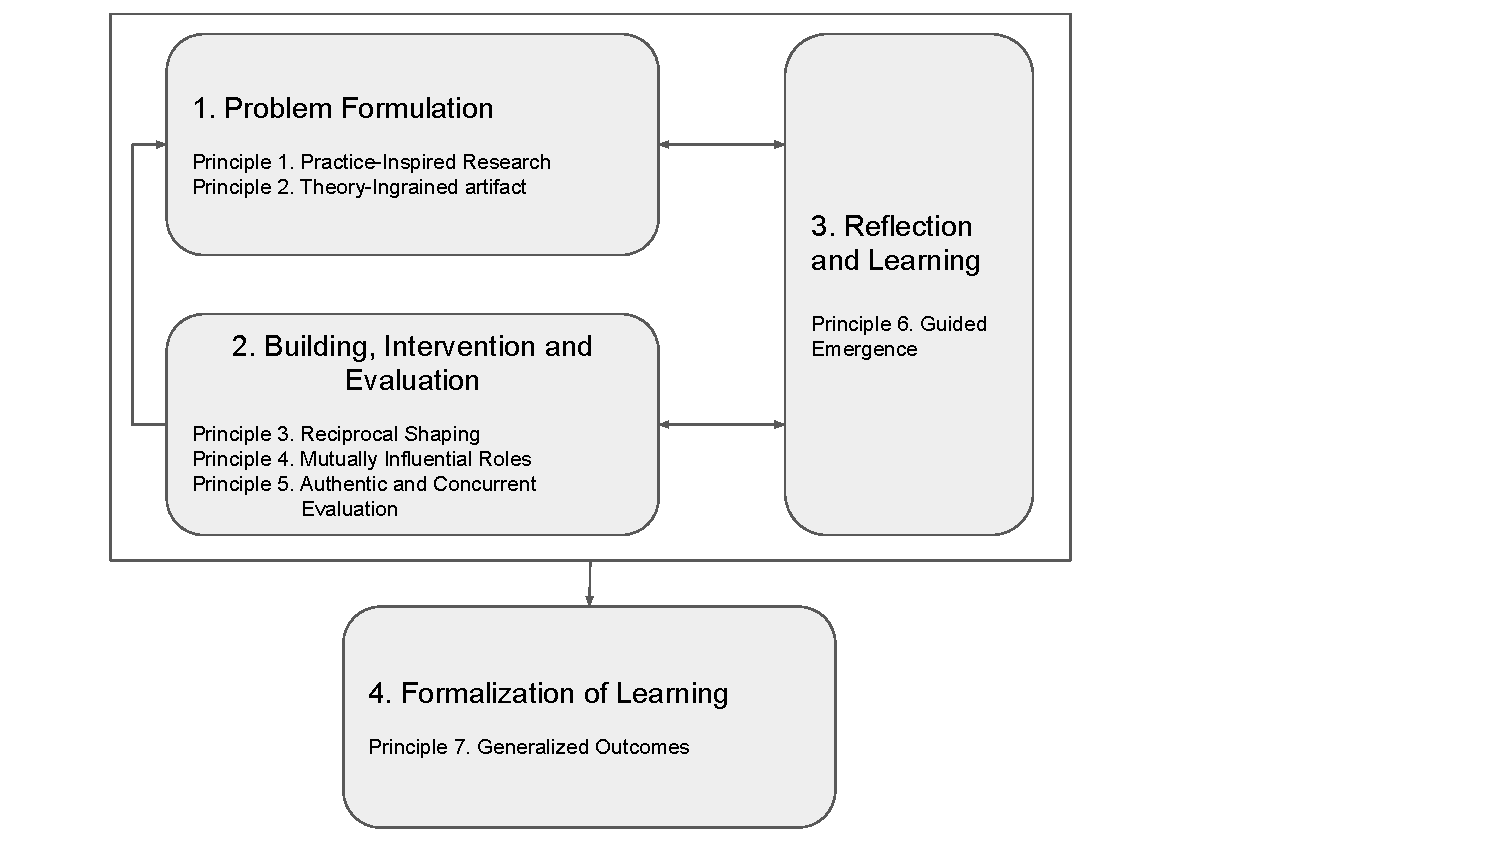
\includegraphics[width=12cm]{diagram/Action_Design_Research_Reproduced.pdf}
\caption{Action Design Research stages and principles \citep[reproduced following][]{Sein2011ActionResearch}}
\label{fig:adr-stages-and-principles}
\end{figure}

ADR stresses the importance of iteration and interaction with the future users of the IT artifact. The Building-Intervention-Evaluation (BIE) cycle enables the interaction, i.e. an artifact is Built and used to implement an Intervention in an organization and to Evaluate the artifact over several BIE cycles. To develop the guidelines for investigating innovation ecosystems as networks as well as the Ostinato Model, we repeat the BIE cycle over series of investigations serving as ADR experiments described in detail in Chapter~\ref{ch:experiments}. The BIE cycle allows us to evaluate the Ostinato Model for validity and added credibility of the presented results. Through guided emergence, we are able to contribute to innovation ecosystem research with deep knowledge of the problem and the proposed solution.

\cite{Sein2011ActionResearch} note that while DSR separates artifact building and evaluation, ADR emphasizes the iterative nature of artifact development. ADR is, therefore, well in line with the principles of contemporary software development approaches. Readers with experience in software development will indeed notice a straightforward connection between the BIE cycle and agile software development \citep[see e.g.][]{Schwaber2001}. More recently, startups and other value-seeking communities within the software development industry have turned their attention to Lean Startup, another iteration-based method \citep{Ries2011}. Apart from the intent to publish the results, these three design and development processes move forward in an iterative and incremental fashion and are guided by feedback collected from the users and other stakeholders of the developed software or other artifact, here ultimately the Ostinato Process Model.

Design science sometimes receives critique for the lack of scientific rigor or bias in practice over theory. ADR responses with the principle of Authentic and Concurrent Evaluation \citep{Sein2011ActionResearch} that we apply through this dissertation. 
% Moreover, to further add to the rigor of the presented research, we will evaluate the research outputs following the core evaluation criteria for qualitative research: credibility, transferability, dependability, and confirmability \citep{Jussila2015SocialInnovation} \todo{Add more references including Guba (1981), Denzin and Lincoln (2000), and Shenton (2004).} 
The utility and viability of artifacts created with the DSR process can be evaluated through proof-of-concept, proof-of-value, or proof-of-use \citep{Nunamaker2011TowardSystems}, each of which adding to the requirements for the state of the artifact as well as the potential level of insight that the artifact has the ability to create. We will revisit the value and use of the artifacts developed in this dissertation as part of the final discussion in Chapter~\ref{ch:discussion}.  

\section{Outline and contributions of the dissertation}
\label{sec:structure}

This dissertation is composed of two complementing lines of investigations. First, a series of innovation ecosystem investigations using visual network analytics is presented. Second, the Ostinato Model, an exploration-automation cycle for a user-centric, process-automated, data-driven visual network analytics is inducted and described.

This dissertation is divided into eight (8) chapters. The 7 articles that together with this summary and synthesis of results form the whole of the dissertation are attached in this dissertation. The contents of each chapter are described briefly below.

Chapter~\ref{chapter:intro} introduces the context of this dissertation, describes the applied research method and epistemological and ontological basis, and specifies the objectives and key contributions of the dissertation.

Chapter~\ref{ch:background} reviews the core literature on the key domains of the dissertation, namely innovation ecosystems, network analysis, and visual network analytics and discusses the fit of the network approach in investigating innovation ecosystems.

Chapter~\ref{ch:experiments} walks the reader through the results of the investigations from the point of view of data-driven visual network analytics. For brevity and tractability of the discussion, we concentrate on the specifics of how visual network analytics were applied in each of the investigations and discuss network-related insights. 

Chapter~\ref{ch:ecosystemnetworks} introduces the first part of the contributions of this dissertation, i.e. the design principles for analyzing innovation ecosystems as networks and creates a synthesis of the way to represent and analyze innovation ecosystems as networks on basis of the investigations as action design research experiments.

Chapter~\ref{ch:processmodels} reviews a set of existing models and takes stock of process model requirements stemming from the experiments to build a foundation for the Ostinato Model. 

Chapter~\ref{ch:ostinato} describes the Ostinato Model for data-driven visual investigations of innovation ecosystem structure.

Chapter~\ref{ch:discussion} discusses the contributions of this dissertation, describes the process through which the contributions emerged and provides a synthesis of the key results.

Chapter~\ref{ch:conclusions} concludes the dissertation and presents directions for further work.
 
This research makes contributions in two complementing levels. First and most importantly, the Ostinato Model for conducting data-driven visual network studies is developed and described. Second, a series of investigations in the field of innovation ecosystem exploratory analysis is conducted, feeding new insights into the emerging phenomena of innovation ecosystems and their research. A concrete outcome of the second contribution is the list design guidelines for representing innovation ecosystems as networks.

In terms of increasing the transparency of the structures emerging from individual transactions and affiliations between innovation ecosystem actors, this dissertation contributes in three levels. First, network analysis is a key approach in supporting exploratory studies on the patterns and structures in between actors founding, working for, advising and investing into startups and growth companies; companies making deals and alliances, investing into and acquiring other companies; and financial organizations investing into startups and growth companies  and in estimating the authority, role and structural position these actors have, therefore allowing for increasing the transparency of the structure of innovation ecosystems of different levels of abstraction from platforms, programs and business sectors to national and international innovation ecosystems. These structures can be modeled, represented, analyzed and visualized as networks to support the investigations and exploration. Second, the presented data-driven approach allows extending these investigations of patterns and structures within and in between groups of actors beyond the boundaries of individual datasets and to happen over long periods of time. Third, actors with different sets of skills from means to crawl online sources for data to domain knowledge allowing deep sensemaking can all fully engage into the different phases of the investigative process.

Moreover, investigations on innovation ecosystems contribute to the body of knowledge on the domain of innovation ecosystem studies with an empirical approach. At the same time, these investigations serve as a vehicle for developing the process model in an incremental and iterative manner following the action design research process.
 
The main contributions of this research are as follows:

\begin{enumerate}[label=\textbf{Contribution \Roman*},align=left]
  \item To meet \ref{objective:empirical}, we contribute to the empirical body of knowledge with a visual description of innovation ecosystems in platform, business domain, development program, national, and international level through a series of investigations. 
  \label{contribution:empirical}

  \item To answer \ref{objective:ecosystemnetworks}, we define a set of design guidelines for modeling and analyzing the structure of innovation ecosystems as networks to support their exploratory analysis.
  \label{contribution:ecosystemnetworks}
   
  \item To satisfy \ref{objective:processmodel}, we define the Ostinato Model for data-driven visual network analytics in the context of innovation ecosystems.
  \label{contribution:processmodel}
\end{enumerate}

% \todo{Link the contributions to specific chapters or sections in the dissertation}

The key result of this dissertation is the introduction of the process model for data-driven visual network analytics in the context of innovation ecosystem investigations. The model is described in detail in \ref{pub:ostinato}.
\chapter{Defining innovation ecosystems, network analysis and visual analytics}
\label{ch:background}

This dissertation operates across three key domains,  innovation ecosystems, network analysis, and visual network analytics. In this chapter, we review the body of knowledge in these domains from the viewpoint of the dissertation.

\section{Innovation ecosystems}
\label{sec:innovationecosystems}

The ecosystem concept has its roots in biology. According to \cite{Moran1990ThePractice}, ``ecosystem generally refers to the structural and functional interrelationships among living organism and the physical environment within which they exist.'' \cite{Moore1993PredatorsCompetition} first introduced the concept to business literature in his seminal article on business ecosystems. The article discusses new ways for companies to allow other companies to create value for them, i.e. the focal company of a business ecosystem. Moore notes that business ecosystems ``condense out of the original swirl of capital, customer interest, and talent generated by a new innovation, just as successful species spring from the natural resources of sunlight, water, and soil nutrients'' \citep{Moore1993PredatorsCompetition}. In business and innovation literature, ecosystem is used both as a metaphor \citep[e.g.][]{Hwang2012,Huhtamaki2011AFinancing}, a business strategy artifact \citep{Moore1993PredatorsCompetition}, as well as to refer to system-level analysis \citep[cf.][]{Pentland2015}.

Innovation ecosystem is a relatively new concept, even when compared to business ecosystem. It is being used in different ways in literature and practical applications. \cite{Hwang2012}, for example, have integrated the ecosystem metaphor in their rainforest framework for ``building the next Silicon Valley.'' To make a distinction between ecosystems of business and innovation in the context of this dissertation, we point to their expected outputs. When the key objective in business ecosystems is to organize value creation and value appropriation in an ecosystem setting, we see that the main output of innovation ecosystems is the increase of information flow and collaboration and therefore the creation of new business-relevant knowledge, ideas and technologies that lead to new products, successful companies and economic growth. In Moore's (\citeyear{Moore1993PredatorsCompetition}) words, innovation ecosystem is the ``swirl'' and its upstream. Innovation ecosystems survive through a constant idea flow, re-configuration, and evolution \citep[cf.][]{Pentland2015}.

Key characteristics of ecosystems are 
interconnectedness, 
interdependency,  
co-evolution, 
value co-creation, and 
co-opetition \citep{Jarvi2016TakingReview,Huhtamaki2011AFinancing}.
Actors in business ecosystems and innovation ecosystems are ``loosely interconnected'' \cite{Iansiti2004TheSustainability}.\footnote{\cite{Iansiti2004TheSustainability} stress that ``like their biological counterparts, business ecosystems are characterized by a large number of loosely interconnected participants who depend on each other for their mutual effectiveness and survival.''} Success of a given innovation often relies on the success of focal companies' environment, i.e. companies are interdependent with each other \citep{Adner2010ValueGenerations}. \cite{Thomas2012ModelingLiteratures} state that co-evolving ecosystem actors ``develop over time sympathetically with the other participants in order to maintain stability and health of the ecosystem in the face of change.''
\cite{Ramaswamy2009LeadingValue} claims that value co-creation is an emerging business and innovation paradigm that leads to the need of ``changing the very nature of engagement and relationship between the institution of management and its employees, and between them and co-creators of value - customers, stakeholders, partners and other employees.'' Finally,
\cite{Ritala2009WhatsCoopetition} note that co-opetition, i.e. collaboration with competitors, is in some cases ``an effective way of creating both incremental and radical innovations, especially in high-tech industries.'' 

\cite{Russell2011TransformingOrchestration} take an even broader scope and define innovation ecosystem as an ``inter-organizational, political, economic, environmental and technological systems of innovation through which a milieu conducive to business growth is catalyzed, sustained and supported.'' They note that in ecosystem level, individual relationships take the shape of a network ``through which information and talent flow through systems of sustained value co-creation.'' Importantly, \cite{Russell2011TransformingOrchestration} include organizational investors and invidual people--founders, advisors, and business angels--as innovation ecosystem actors (and therefore potential units of analysis in innovation ecosystem investigations) \cite[cf.][]{Huhtamaki2011AFinancing}.

To manage innovation ecosystems as well as to facilitate their emergence, the process of network orchestration is encouraged \citep{Russell2015RelationalEcosystems}. In all, innovation ecosystems are rather orchestrated than controlled or managed \citep{Russell2011TransformingOrchestration,Ritala2009,Ritala2013,Paquin2013}. When collective gains are sought at the network level, change agents seek to facilitate the emergence of networks, orchestrate existing networks and manage their growth \citep{Russell2011TransformingOrchestration}. A dynamic innovation ecosystem is characterized by a continual realignment of synergistic relationships that promote growth of the system \citep{Russell2015RelationalEcosystems}.

Innovation ecosystem research can take place in three different levels \citep{Jarvi2016TakingReview}: ``the individual actor, the relationship between actors and the ecosystem as a whole.'' We claim that system-level view is imperative in investigating, navigating, and orchestrating innovation ecosystems. With \cite{Jarvi2016TakingReview} as evidence, we note that during the writing of this dissertation, empirical ecosystem-level research on business and innovation ecosystems is scarce, very likely due to the mismatch between knowledge demand and the the existing methods that are perhaps better suited to conduct analysis in actor and relationship level.

Discussion on the utility of the innovation ecosystem as a concept is ongoing. A recent critique of the concept \citep{OhInnovationExamination} states that the eco-prefix in ecosystem may only add to the difficulties in communication related to research and its application in decision-making. The ecosystem as a metaphor is powerful and therefore prone to misconception and preposterous thinking \citep{OhInnovationExamination}. At the same time, scholars continue to seek the extent in which the biological ecosystem concept can indeed applied. The study on the technospecies concept \citep{Weber2015WhoConcept} is an example of the latter approach. In this dissertation, we are first and foremost interested in the properties that scholars and decision-makers attach to innovation (eco)systems and the ways the investigations of these properties can be conducted with a data-driven visual network analytics approach. In fact, we believe that empirical research can help to take the discussion to more concrete level and provide means to test the validity of innovation ecosystem theory. 

In the experiments included in this dissertation, we investigate innovation ecosystems with a Silicon Valley-style mindset. This means that we do not limit the investigation into companies and their interconnections. Instead, we study the structures that emerge from activities taking place around startups, the individuals that found, advice, invest into, and work in key positions for the startups. Also growth companies that have already crossed the death valley of company growth and continue to evolve toward a liquidity event, e.g. exit through an acquisition or Initial Public Offering (IPO) are of our interest. For context, we also study the already established enterprises and deals and alliances connecting them with each other. Moreover, we seek ways to explore the role of individual customers as well as organizations that facilitate the creation and growth of the companies in the core of our investigations.

\section{Network analysis}
\label{sec:networkanalysis}

Innovation ecosystems are studied in this dissertation with visual network analytics. In network analysis, phenomena under investigation are modeled as nodes and edges representing the entities and their interconnections. We fully subscribe to \cite{Yang2014OverlappingNetworks} in that ``Networks provide a powerful way to study complex systems of interacting objects.'' 
 
Network analysis has its roots in social network analysis (SNA) \citep{Moreno1953,Wasserman1994SocialApplications}. While the first applications of network analysis dates back to 1950's and Milgram's famous experiment that gave evidence on the small-world nature of the world was reported in \citeyear{Milgram1967TheProblem} \citep{Milgram1967TheProblem}, network analysis remains a relatively new method for a number of domains. Key steps in network science include the introduction of a model for generating small-world networks \citep{Watts1998,Watts1999} and the discovery of scale-free networks \citep{Barabasi1999EmergenceNetworks}. The availability of interesting real-life social data and the development of computing capabilities have significantly increased the potential for applying network analysis in investigating various phenomenon \citep[cf.][]{Hansen2011AnalyzingWorld,Bastian2009Gephi:Networks}.

Social network analysis studies the social structures of actors. Sociogram is the core artifact in social network analysis. \cite{Wasserman1994SocialApplications} define sociogram as ``a picture in which people (or more generally, any social units) are represented as points in two-dimensional space, and relationships among pairs of people are represented by lines linking the corresponding points.'' The network structure is key to understanding the complex system of relationships \citep{Barabasi2003Linked:Means}: ``Small changes in the topology, affecting only a few of the nodes or links, can open up hidden doors, allowing new possibilities to emerge.''

A phenomenon under investigation can be modeled either as one-mode, two-mode, or multimodal network. In one-mode networks, all the nodes are of same type. Among company board members, for example, connections between the nodes are formed on basis of friendship or, in innovation ecosystem context, on the basis of company board co-membership. In two-mode networks, there are two types of nodes. A two-mode network of company and investor would show a company node connected to each investment firm from which it has received funding. Means to visualize two-mode networks include hypergraphs and bipartite graphs \citep{Freeman2000VisualizingNetworks, Jesus2009}. The connections may be undirected or directed, the latter resulting into a digraph. Further, the connections between the actors can be either dichotomous or weighted, in which the strength of a connection can be expressed.

The analysis of overall network structure, the different characteristics of the network, the roles of the network actors, and the nuances of their interaction are of interest in many fields of research. The actors in networks, acting as hubs or connectors, may be characterized as random, small-world \citep{Watts1998,Milgram1967TheProblem} or scale-free \citep{Barabasi2003} as they diffuse information within the network \citep[cf.][]{Molka-Danielsen2007IRISAnalysis}. Process phenomena such as preferential attachment \citep{Barabasi1999EmergenceNetworks}, homophily, reciprocity and transitivity \citep[cf.][]{Giuliani2008} shape the networks as they evolve.

Precise SNA metrics can be calculated for all three units analysis in innovation ecosystem investigations: network actors, connections between the actors as well as the network as a whole. Node degree representing the number of connections of a node is the simplest metric. Main categories for actor SNA metrics are centrality and prestige \citep{Wasserman1994SocialApplications}. Key metric for connections is their weight. Metrics such as density and cohesion \citep{Hansen2011AnalyzingWorld} describe networks quantitatively.

Network analysis has been applied to investigate companies and different company-related phenomena. Co-creator networks have been one of the early applications of visual social network analysis. When reviewing the historical and theoretical foundations of SNA, \cite{Freeman2009MethodsVisualization} refers to early work of Hobson who already in 1884 ``produced a visual image of a social network that was not based on kinship.'' Unlike his predecessors, Hobson designed a two-mode network of corporations and their directors with, as \cite{Freeman2009MethodsVisualization} interprets, the rationale ``that, to the degree that corporations shared directors, they could be expected to cooperate and work together.'' Another example of an early visual investigation of corporate networks is Levine's work on ``corporate interlocks'' as relationships through which social norms influence information flow for business intelligence \citep{Levine1979Joint-spaceAlternatives}. The notion of weak ties \citep{Granovetter1973TheTies} is another important landmark in applying network analysis to sociological research in studying business and economy. \cite{Olson2008GreatAPI} reports a more recent example of visualizing corporate interconnections implemented with socially constructed data. \cite{Basole2009VisualizationEcosystem} applies visual network analysis to analyze interfirm relations in the mobile ecosystem and gives an extensive review of literature on visual network analysis in business studies. Importantly, innovation ecosystem studies that utilize network analysis are almost non-existing outside the ones included in this dissertation.

Examples of innovation ecosystem investigations with a network-centric mindset are rare outside the works of the authors and his collaborators. There is, however, an increased interest toward analyzing innovation ecosystems as network. Recent examples of this include \cite{Clarysse2014CreatingEcosystems} and \cite{Parise2015HowIdeas}.

\section{Visual network analytics}

Due to the complexity of business ecosystems, derivation of conceptual insights from business ecosystem data is challenging \citep{Bizzi2012StudyingNetworks,Basole2015UnderstandingApproach}. These challenges exist in innovation ecosystems as well and the openness of the latter further adds to these challenges. Visual revelation of patterns in complex ecosystem data allows for gaining important knowledge of the patterns and dynamics of [innovation] ecosystems \citep{Basole2013UnderstandingVisualization}.

While a statistical analysis provides valuable insights to the structure and dynamics of ecosystems, important knowledge can also be gained through the visual revelation of patterns in a complex business ecosystem data \cite{Basole2013UnderstandingVisualization}. Indeed, visualizations are more than merely artistic approaches to depicting structure in helping investigators to explore the data throughout the analysis process \citep{Fox2011ChangingVisualization}. Visualizations have been used to explore, interpret, and communicate data in order to aid humans in overcoming their cognitive limitations, making structure, patterns, relationships, and themes visible, and providing a means to efficiently compare multiple representations of data in similar fields such as medicine, dentistry, computer science and engineering. \cite{Tufte1983VisualInformation} suggests that when applied properly, visualization is an extremely valuable tool for understanding and analyzing business issues, including strategy, scenario planning, and problem-solving.

Visual analytics is used in this dissertation to negotiate issues related to complexity to gain knowledge on innovation ecosystem ``through the visual revelation of patterns'' \citep{Basole2013UnderstandingVisualization}. We claim that visual analytics allows for understanding and analyzing issues related to business and innovation alike through scenario-planning and problem-solving \citep{Tufte1983VisualInformation}.

We are exited to observe the existence of individual pieces of literature taking note on the development of analytics-based insights that go beyond quantitative (causal) relationships of individual measurements \citep{Bygstad2011InAnalysis,Bendoly2016FitAnalytics,Williams2015MixedAnalysis}. In the context of information systems research, \citep{Bygstad2011InAnalysis} present a critical realist-inspired analytical framework for identifying socio-technical mechanisms in a way that allows for ``ontological depth, creative thinking and more precise explanations'' that goes beyond traditional statistical analysis. \cite{Williams2015MixedAnalysis} remind of the interdisciplinary origins of social network analysis and present a framework for processing data from multiple sources including archival records for network analysis with a mixed methods approach. \cite{Bendoly2016FitAnalytics} put visual analytics into the center of stage in data analytics, from data validation and curation through exploration and discovery to end-result communication and (re-)interpretation. Further, \citeauthor{Bendoly2016FitAnalytics} points to the importance of ``not just simultaneous parallel use [of data and visualizations] but truly joint utilization and team-wise sensemaking for effective decisions.''

With visual network analytics, we refer to taking a visual analytics \citep{Thomas2006AAgenda,Heer2012InteractiveAnalysis} approach to network analysis. Visual analytics stresses the process-centric, interactive nature of using visualizations in supporting data-driven investigations \citep{Keim2010MasteringAnalytics,Heer2012InteractiveAnalysis}. Visual analytics is a particularly suitable approach for exploring new phenomenon with a data-driven approach. Visual network analytics allows the emergence of insights on the structure and dynamics of business and innovation ecosystems \citep{Basole2009VisualizationEcosystem}, social media platforms \citep{Smith2015TheConversations} and other networked phenomena. Transforming those insights into action, however, requires communicating the insights to constituents of change \citep{Russell2011TransformingOrchestration,Still2014InsightsVisualisations}. Visual network analysis is a valuable method for investigating social configurations and for interactively communicating their findings to others \citep{Freeman2000VisualizingNetworks}.

The well-known mantra of visual information retrieval iterates over three phases: ``Overview first, zoom and filter, then details-on-demand'' \citep{Shneiderman1996TheVisualizations}.
In the context of visual network analysis, however, users may prefer to follow the process of ``start with what you know, then grow'' \citep[][p. 35]{Heer2005}. Visual analytics theory suggest that, at best, an investigator of a phenomena is able to interact with all the phases of the process from view creation to exploration and refinement in an expressive manner \citep{Heer2012InteractiveAnalysis}.

A data-driven process for understanding the roles of the different actors in an innovation ecosystem allows for interactive discovery to support both investigation and orchestration of innovation ecosystems \citep{Russell2015RelationalEcosystems}. Multiple perspectives on ecosystem structure and the structural positions of individual actors can be invited and exchanged during the investigative process. With subsequent automation of data updates and tracking analyses, the assumptions and contingencies underlying decisions can be monitored for changes that would impact policy and program directions.

In the experiments included in this dissertation described in detail in Chapter~\ref{ch:experiments}, we use network nodes to represent innovation ecosystem actors. The actors are connected to each other on basis of different kinds of transactions between them. These transactions include investments, acquisitions, deals and alliances. Moreover, key individuals are connected to companies they are or have been affiliated with. Network metrics are used to quantify the structural positions of these actors. Network representations are laid out in a way that allows their visual investigation. Visual properties of network nodes and edges are specified in a way that supports these investigations.

% Very little literature exists on visual (network) analytics of innovation ecosystems. Searching Scopus in April 2016 for (visual  analytics  OR visual  analysis  OR  visualization) AND (innovation ecosystem OR innovation ecosystems) gives only 17 results, including three articles which the author of this dissertation has co-authored.

\section{Cognitive fit of network analysis}

Network representation of information is utilized extensively in information systems. Indeed, network representation of information is at the core of hypertext. When presenting the notion of the hyperlink, Vannevar Bush highlights the similarity in between network representation and the way the human mind operates \citep{Bush1945AsThink}: 

\begin{quote}
``The human mind [...] operates by association. With one item in its grasp, it snaps instantly to the next that is suggested by the association of thoughts, in accordance with some intricate web of trails carried by the cells of the brain. It has other characteristics, of course; trails that are not frequently followed are prone to fade, items are not fully permanent, memory is transitory. Yet the speed of action, the intricacy of trails, the detail of mental pictures, is awe-inspiring beyond all else in nature.''
\end{quote}

We claim that representing innovation ecosystems as networks allows for an intuitive way to investigate and revisit data representing innovation ecosystems. Indeed, \cite{Bush1945AsThink} added that ``[m]an cannot hope fully to duplicate this mental process [the intricacy of trails in human mind] artificially, but he certainly ought to be able to learn from it.'' In this dissertation, we taken advantage of existing sources of digital data on innovation ecosystem actors and transactions and affiliations between them to recreate these traces to allow for system-level views of the currently scattered innovation ecosystem landscape. To reuse McGonigal’s \citeyearpar{McGonigal2005} insightful metaphor inspired by Lewis Carroll, we see visual network analytics as meas to craft ``rabbit holes'' through which innovation ecosystem explorers are drawn into new information landscapes beyond their imagination to find new, interesting ideas, companies, investors, communities or a similar-minded innovation champions \citep[cf.][]{Huhtamaki2007CommunityEcosystem} or emerging patterns that give competitive edge to a company, ecosystem, program, region or nation.

Cognitive fit theory suggests that in supporting problem-solving and decision-making, it is particularly important to find a fit between the problem-solving task and the problem representation and supporting tools; cognitive fit allows for faster and more accurate performance in decision-making \citep{Vessey1991}. There is a delicate balance in developing tools with cognitive fit, however: experimental research shows that neither the time used to conduct a task nor the confidence that the users feel about their decisions are good predictors of the accuracy of their insights or decisions \citep[cf.][]{Dunn2001}. Cognitive fit theory further suggests that when the problem representation fits the problem-solving task, a preferable and more consistent mental representation of the problem will be realized, thereby facilitating the problem solving process, and consequently resulting in preference for the representation, along with faster and more accurate performance in decision-making \citep{Basole2016EnablingAnalysis}.

Using network analysis in the context of investigating and orchestrating innovation ecosystems is closely related to relational and social capital theory. In their seminal article on social capital\footnote{\cite{Still2013relationalsocialcapital} show that \cite{Nahapiet1998} is a key article in between social capital and relational capital research.} \cite{Nahapiet1998} introduce a third dimension  for social capital to complement the relational (relationship-level social capital) and structural dimension (system-level social capital) and label that as cognitive dimension to refer ``to those resources providing shared representations, interpretations, and systems of meaning among parties.'' \cite{Nahapiet1998} ``believe it represents an important set of assets not yet discussed in the mainstream literature on social capital but the significance of which is receiving substantial attention in the strategy domain.''

From relational capital research viewpoint, this dissertation seeks to use visual network analytics to augment the cognitive dimension of ecosystemic relational capital \citep{Still2014EcosystemicRelationalCapital}.
% \include{innovationecosystems}
% \include{networkanalytics}
\chapter{Experiments in investigating innovation ecosystems}
\label{ch:experiments}

In this chapter, we give an overview of the individual experiments on investigation innovation ecosystems with data-driven visual network analytics. In the context of this dissertation, the experiments serve first and foremost as means to develop the approach and methodology for investigating innovation ecosystems as networks, i.e. to distill design principles and process requirements in interaction with innovation ecosystem actors, stakeholder, decision-makers and investigators through the process of guided emergence \citep[cf.][]{Sein2011ActionResearch}. Moreover, the results and insights contribute to \ref{objective:empirical} of the dissertation.

The experiments are conducted on innovation ecosystems representing different levels of abstraction and complexity from Demola platform, a local ecosystem engager, to EIT ICT Labs (currently operating as EIT Digital), a large international ``open innovation organisation''\footnote{EIT Digital, \url{http://eit.europa.eu/eit-community/eit-digital}}. In all of the experiments, we take a data-driven approach to explore and describe the structure and in some cases structural dynamics of the innovation ecosystems under investigation.

The innovation ecosystems in which the experiments take place represent a broad range of abstraction and complexity. For specificity, we present the following categorization for the innovation ecosystems:

\begin{itemize} 
  \item Platform level: Demola
  \item Business domain level: Mobile Ecosystem 
  \item Program level: Tekes Young Innovative Companies\footnote{Tekes Young Innovative Company funding programme, \url{http://www.tekes.fi/en/funding/yic/}}
  \item National level: Finnish Innovation Ecosystem
  \item International level: EIT ICT Labs
\end{itemize}

Here, we will review the experiments from local to global. We want to note, however, that the order in which the experiments were conducted is different from the categorical order. Finnish Innovation Ecosystem was the first experiment. Second, the investigation of the mobile ecosystem was conducted. Third, we took a network approach to investigate the ecosystem emerging through Tekes Young Innovative Companies program. Fourth, means to use visualization to support orchestration of EIT ICT Labs were investigated. Fifth, we revisited the Finnish Innovation Ecosystem with a multiscopic approach. Sixth and finally, the evolution of innovation ecosystem operating on the Demola platform was investigated. Table \ref{tab:experiments} describes the individual experiments in more detail.
 
For tractability and presentation brevity, we review the experiments specifically from network analysis viewpoint and address the findings that are related to the design decisions on network analysis of the innovation ecosystems.

% http://tex.stackexchange.com/questions/62875/captionof-messes-with-paragraph-indent
\begingroup
\captionof{table}{Overview of the investigations}\label{tab:experiments}
\begin{tabular}{p{2.5cm} p{4cm} p{5.5cm}}
\textbf{Ecosystem} 
& \textbf{Data} 
%& \textbf{Co-creators} 
& \textbf{Key outputs} \\

Demola (\ref{pub:demola}) &
Proprietary data on Demola projects, the companies that initiated the project and university affiliations of project members (university students) & 
% Demola leaders and operators and the investigative team & 
The animation of the evolution of Demola project sphere including projects, companies and the affiliations of project team members. Multimodal networks of 1) projects and affiliated actors and 2) projects and their key competences \\

Mobile Ecosystem (\ref{pub:mobileecosystem}) &
Thomson Reuters SDC and Innovation Ecosystems Network (IEN) Dataset  & 
% The investigative team & 
Dataset-specific visualizations of the innovation ecosystem surrounding pairs of ecosystem actors (Nokia and Microsoft, Google and Motorola Mobility) \\

Tekes Young Innovative Companies (\ref{pub:tekesyic})  &
IEN Dataset on growth companies, Twitter data on Tekes Young Innovative Companies (YIC) and their followers & 
% Policy makers at Tekes - the Finnish Funding Agency for Innovation and the investigative team & 
One and two-step networks of the companies taking part in Tekes YIC program and their affiliations to investors and key individuals \\

Finnish Innovation Ecosystem (\ref{pub:finland}) & 
IEN Dataset on growth companies & 
% Finnish national-level policy makers and the investigative team & 
Network visualizations and metrics on Finnish companies and their first-step connections to other companies, investors and key individuals \\

Finnish Innovation Ecosystem (\ref{pub:multiscopicfinland}) & 
Three separate datasets: 1) Thomson Reuters SDC for deals and alliances and IEN Dataset for 2) Executives and Finance and 3) Startups and Angels & 
% Finnish national-level policy makers and the investigative team & 
Network visualizations and metrics on companies having their main office in Finland and their first-step connections to other companies, investors and key individuals \\

EIT ICT Labs (\ref{pub:eitictlabs}) & 
IEN Dataset for Executives and Finance	& 
% EIT ICT Labs representatives and the investigative team & 
Network representation of EIT ICT Labs co-location cities and their first-step connections to investors, individuals and other companies
\end{tabular}
\endgroup

\section{Platform level: Demola}

In innovation platform level, we investigate Demola, an ecosystem engager that facilitates collaboration in between universities and companies. The investigation focuses specifically to Demola Tampere site, the original location of the platform that in 2016 has spread to more than ten locations worldwide\footnote{Demola – Building The World’s Strongest Innovation Ecosystem, \url{http://www.demola.net/}}. Demola is an innovation ecosystem engager, an open innovation platform that takes real-life problems from companies and other organizations and puts together and facilitates projects where students from different universities collaborate to solve the problems. 

In \ref{pub:demola}, we \citep{Huhtamaki2013ProcessDemola} describe a set of network visualizations and animations that are developed in co-creation with the Demola operators with the objective to make the Demola-initiated activity visible. Moreover, the development process used to design the visualizations and the technical process is described and discussed in the article. We claim that static network visualizations and, importantly, the animations of the evolution of an open innovation platform development are useful in presenting, describing, marketing and selling the platform for existing and new stakeholders. Figure~\ref{fig:animating-demola} shows a snapshot of the animation of the evolution of Demola project sphere. Our experience in the experiment suggests that in order to develop visualizations and animations that meet the requirements set by the different stakeholders, an iterative and incremental development process is needed. Moreover, we claim that taking a data-driven approach to visualization development is a key enabler in supporting the development process.

\subsection{Rationale for network analytics}

Open innovation breaks the traditional pattern for developing new innovation leading to new business and the activities toward it and, consequently, new requirements are posed to measuring innovation \citep[cf.][]{Still2012ParadigmDigital}. For an ecosystem engager like Demola, many of the traditional innovation metrics, e.g. change in company turnover, the number of patents, companies or scientific publications created, or the amount of new product launches, cannot be easily tracked down to individual projects or even to companies' engagement with Demola in general. In fact, many Demola stakeholders see these outputs to be less relevant to the core activity. At the same time, Demola needs to communicate about its activities and impact both internally and externally.

In this investigation, we joined with members of the Demola operating team to design ways to represent the structure and dynamics of the Demola platform. The investigative team made an inventory of the key challenges that Demola representatives face in measuring and communicating their innovation activities and their impact. The majority of visualization and animation development was conducted by a team of three including 1) a person with deep knowledge on Demola vision, mission and strategy, 2) a person with specific knowledge of the existing system used to manage project data, and, 3) a person with knowledge on applying visual network analytics for innovation ecosystem analysis and visualization.

Taking the network approach allowed us to reuse and refine some of the existing processes developed for investigating other innovation ecosystems to the context of an individual open innovation platform.

\subsection{Data sources}

Demola runs a dedicated web-based platform for setting up new projects as well as for running existing ones. During the first planning sessions, it became evident that the data Demola already collects and produces provides a useful representation of the structure and evolution of the ecosystem.

For this investigation, we concentrated solely on the in-house project data. The data was exported from the Drupal-based Demola platform with a tailored batch script and serialized in CSV (Comma Separated Values) format for further processing. Demola operating team curated the project data to meet the needs of the visualization process. Particularly the naming of project themes required harmonization.

\subsection{Network modeling decisions}

Projects, collaboration partners, project team members and their universities are all intuitive candidates to be used as network nodes. In addition, we decided to use nodes for representing the project key areas. Figure \ref{fig:animating-demola} presents a screen capture of the key output of the experiment, an animation of the evolution of the network structure of Demola Tampere ecosystem.

\begin{figure}[htb]
\centering
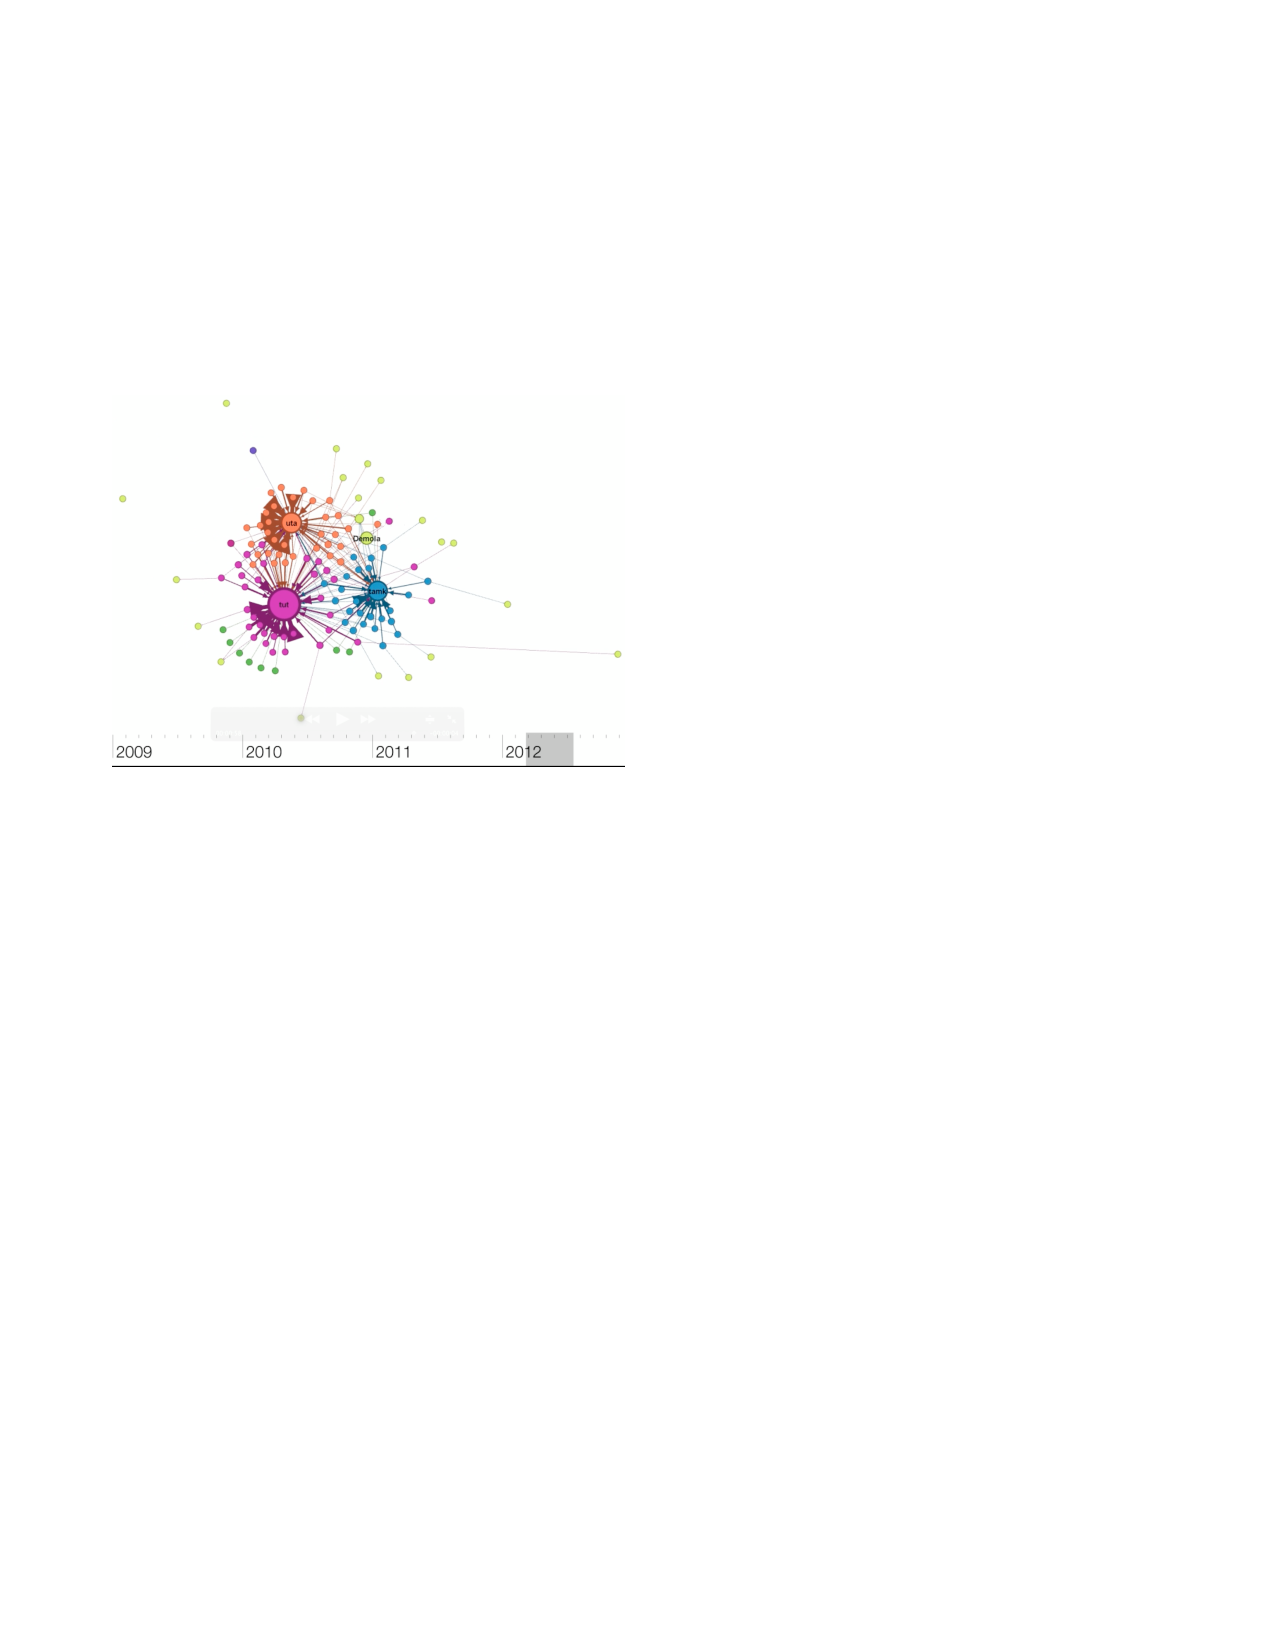
\includegraphics[width=12cm]{figure/Animating-Demola-Evolution.pdf}
\caption{Innovation platform Evolution: Animating Demola Evolution \citep{Huhtamaki2013ProcessDemola}}
\label{fig:animating-demola}
\end{figure}

Network Analysis and Visualization (NAV) process model \citep{Hansen2012DoData} is used to frame the analysis process. The implementation of the visualization process is an interplay between tailored code and the use of pre-existing tools. Python and NetworkX are used to pre-process the data and the visualizations and the animation are created with Gephi.

In network in Figure \ref{fig:animating-demola}, node size represents its betweenness value and edge weight shows the number of students affiliated with a particular university. Node colors represent network clusters. Force-driven algorithm is used to lay out the nodes. To show the dynamics of the Demola platform, edges connecting companies to individual projects only exist during the going of the project after which the layout algorithm starts pushing loose nodes away from the center. When force-driven layout is run in real time, the animation shows for example the retention patterns of individual companies engaging with the platform. Capturing of the video was done with a screen-recording software and timeline was included during post-production.

\subsection{Results and network-related insights}

The key output of the Demola investigation is the animation of the evolution of Demola Tampere Ecosystem from its first day of operation to the beginning of year 2013 when the investigation was conducted.

On basis of the feedback received both during the co-creation process as well as after the publishing the study, we claim that particularly the dynamic animation of the platform evolution is useful in presenting, describing, marketing and selling the platform for existing and new stakeholders. As evidence, we offer the fact that Demola operating team has continued to use the animated project network as a tool for communicating Demola activities and their evolution over time.

\section{Business domain level: mobile ecosystem}

The mobile ecosystem consists of a heterogeneous and continuously evolving set of companies that are interconnected through a complex, global network of relationships. There is however very little theoretical understanding on how these networks emerge and evolve and no well-established methodology to study these phenomena. Traditional approaches have primarily utilized alliance data of relatively established firms; however, these approaches ignore the vast number of relevant ecosystem activities that occur at the personal, entrepreneurial, and university level. In \cite{Basole2012UnderstandingApproach}, we argue and empirically illustrate that a data-driven approach can provide important complementary explanatory insights into the dynamics of the mobile ecosystem. We present our approach through two mobile ecosystem relationships that were formed just before the investigation--the strategic partnership between Nokia and Microsoft and Google’s acquisition of Motorola Mobility. Our analysis is complemented with network visualizations. The article concludes with implications and future research opportunities, some of which we ourselves took up in an extended version of the article \citep{Basole2015UnderstandingApproach}. 

This investigation was conducted without external stakeholders.

\subsection{Rationale for network analytics}
% * <jukka.huhtamaki@tut.fi> 2015-07-01T08:32:10.055Z:
%
%  Should we refer to analysis (rather than analytics) when we refer to individual analysis cases rather than the more general process used to conduct the individual analyses?
%

The investigation stems from the fact that there is very little theoretical understanding on how ecosystems emerge and evolve \citep{Ahuja2012TheNetworks}. Network modeling is an integral part of investigating ecosystems in system level. Companies, investors, and invididuals are represented as network nodes and their interconnections are tracked over time to analyze the emergence of ecosystem patterns. Snapshots of the structure are used to analyze the evolution of the structure. We admit that network analysis alone is not enough in developing rich insight on structures and mechanism underlying emergence and evolution and propose further investigations based on agent-based modeling \citep[cf.][]{Huotari2016WinnerMarkets}.  

\subsection{Data sources}

The ecosystems surrounding the pairs of companies are investigated with two complementing datasets. First, we use Thomson Reuters SDC Platinum, an institutionally curated dataset on deals and alliance between already established companies, for transactional microdata on the direct and second-tier connections of the pair of companies. Second, to add to the insights on startups and growth companies, venture capital investors and even key individuals, we tap into IEN dataset for complementary views into the ecosystem. IEN Dataset is a collection of socially constructed datasets on executives, finance, business angels and startups \citep{Rubens2010LeveragingMoves}.

\subsection{Network modeling decisions}

Figure~\ref{fig:mobile-ecosystem-sdc} shows the ecosystem surrounding Google and Motorola Mobility based on Thomson Reuters SDC data. In Figure~\ref{fig:mobile-ecosystem-iend}, the startup and growth company centric view of the ecosystem surrounding Google and Motorola Mobility is shown. Separate networks are created to represent ecosystem structure emerging from Thomson Reuters SDC (e.g. Figure~\ref{fig:mobile-ecosystem-sdc}) and IEN Dataset (e.g. Figure~\ref{fig:mobile-ecosystem-iend}). In previous, nodes represent companies and, in latter, companies, investors and individuals. In previous, companies are connected on basis of joint deals and alliances. In latter, companies are connected to investors, key individuals and other companies that have either acquired or invested in a company. 

\begin{figure}[htb]
\centering
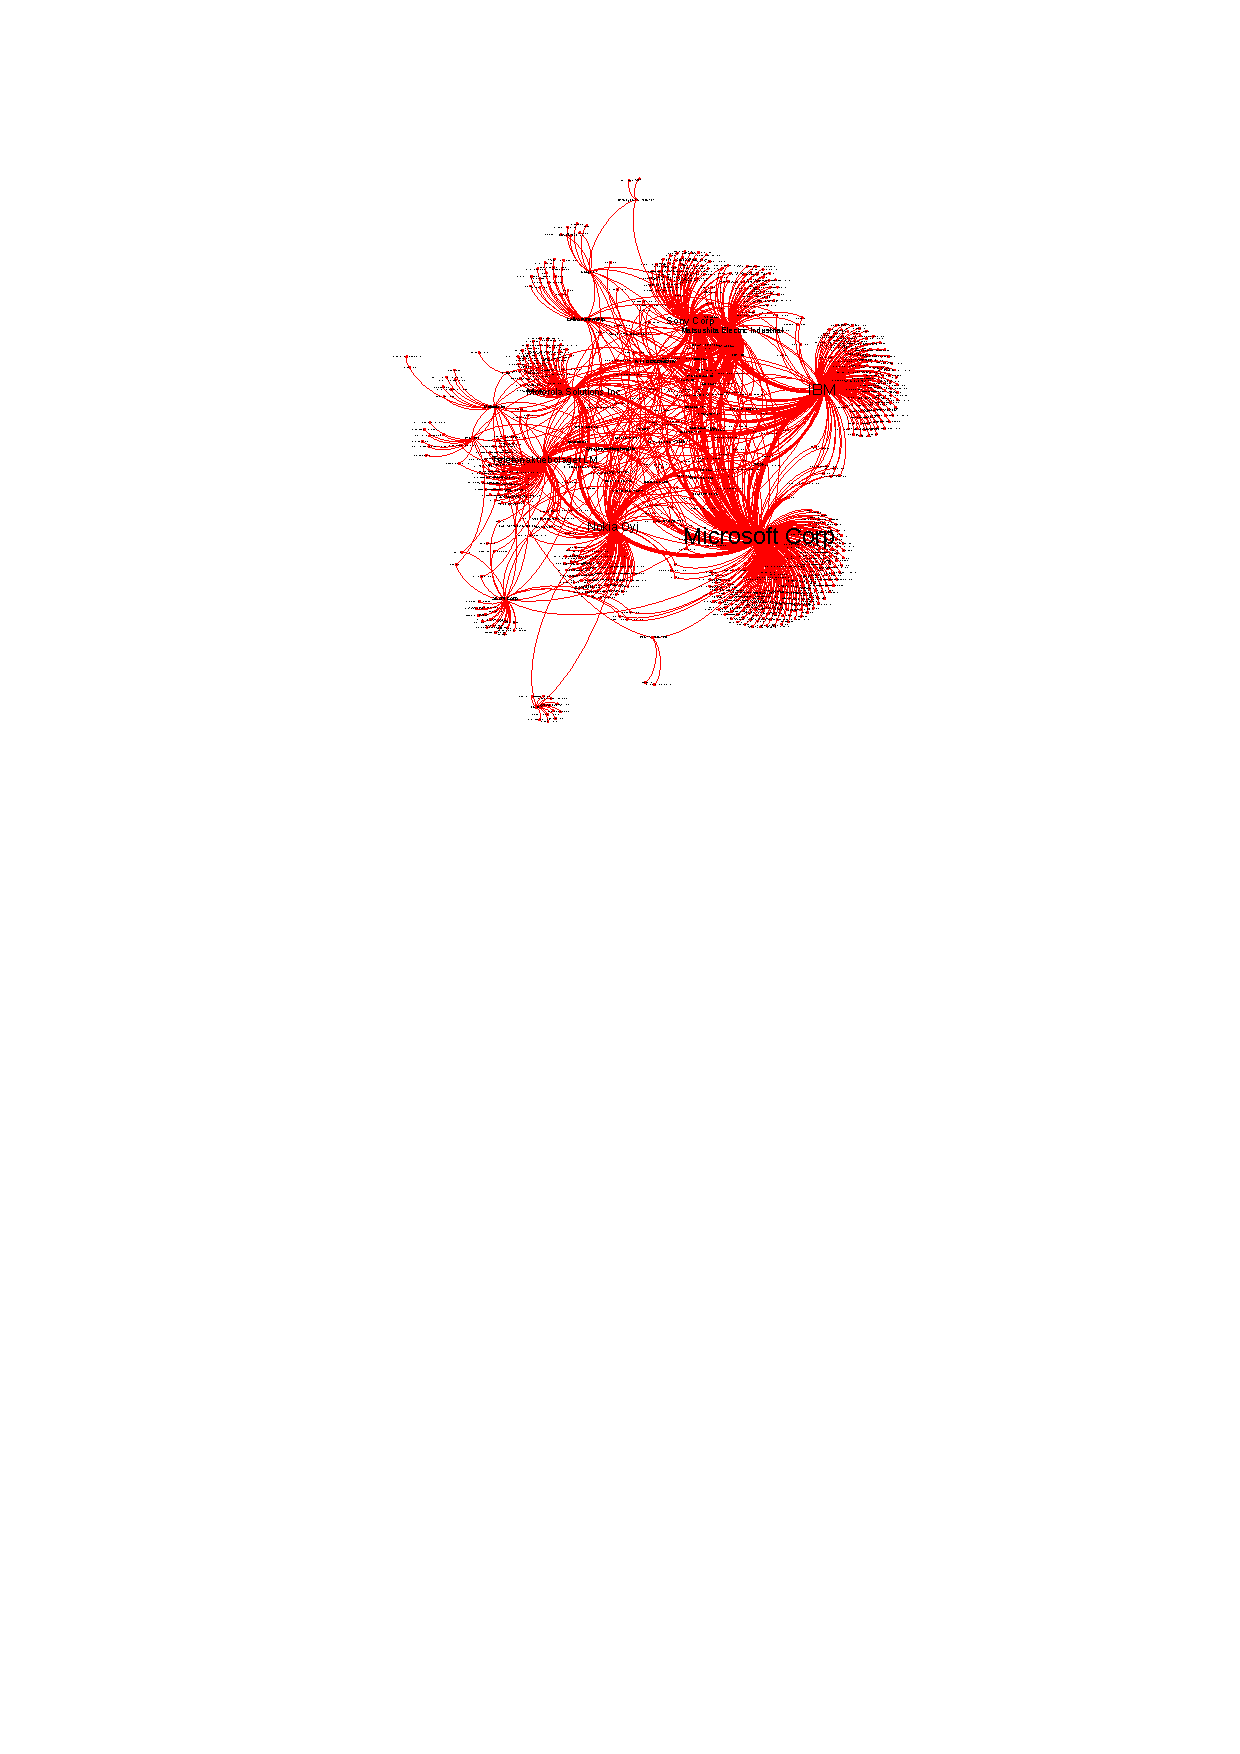
\includegraphics[]{figure/Mobile-Ecosystem-Google-Motorola-SDC.pdf}
\caption{Cumulative network around Google and Motorola Mobility using Thomson Reuters SDC data for deals and alliances. Through second-step connections, Microsoft becomes the key node in the network. \citep{Basole2012UnderstandingApproach}}
\label{fig:mobile-ecosystem-sdc}
\end{figure}

\begin{figure}[htb]
\centering
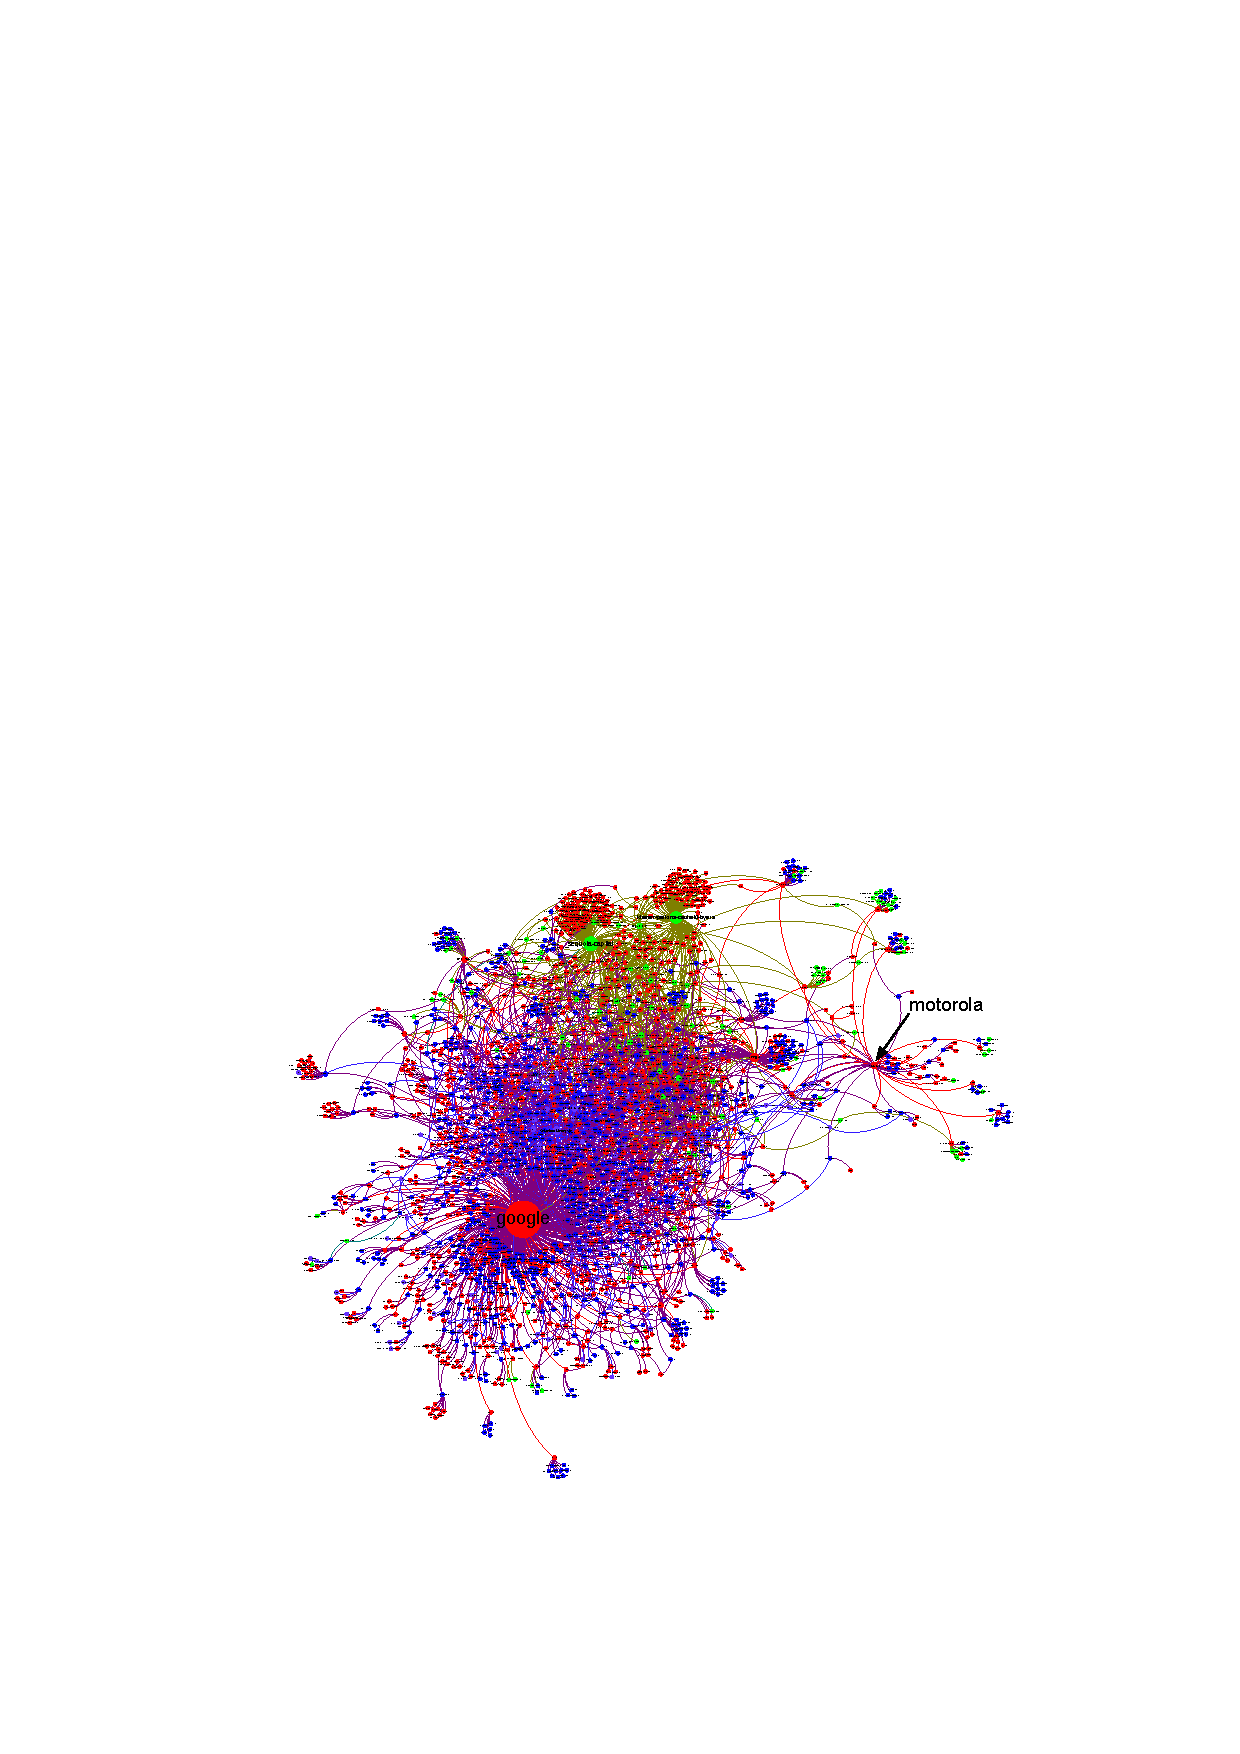
\includegraphics[]{figure/Mobile-Ecosystem-Google-Motorola-IEND.pdf}
\caption{Cumulative network around Google and Motorola Mobility. Google's approach to operating through acquisitions rather than deals and alliances (cf. Figure~\ref{fig:mobile-ecosystem-sdc}) is highlighted. \citep{Basole2012UnderstandingApproach}}
\label{fig:mobile-ecosystem-iend}
\end{figure}

Boundary specification includes the selection of nodes, node types and relationship types, analysis timeframe, as well as the steps from focal companies to include other companies and stakeholders \citep{Basole2012UnderstandingApproach}. In this investigation, all companies and other actors within two steps from the focal companies are included in the network. Force-driven algorithm is used to lay out the network.

For investigating the evolution of the structural properties of the ego-centric networks, we created snapshots of the networks and calculated the development of a set of node and network-level metrics over time. These measurements are represented as small multiples in the article.

\subsection{Results and network-related insights}

Two illustrative investigations exemplify the use of the data-driven approach for understanding the mobile ecosystem. In February 2011, Nokia and Microsoft announced a strategic alliance to work together in developing their mobile offering, both in terms of devices as well as an ecosystem feeding applications and other content to add value to device users. Google acquired Motorola Mobility in August 2011 to strengthen its capabilities in the mobile domain.

Separate network representations are created for the two set of data as well as the two cases. Figure \ref{fig:mobile-ecosystem-sdc} shows the 2-step network of Google and Motorola mobility with Thomson Reuters SDC Platinum data representing the ways that traditional enterprises operate. Even though not a focal company in this representation, Microsoft emerges as the supernode in the network. With network representation of IEN Dataset in \ref{fig:mobile-ecosystem-iend}, Google's true size accumulated particularly through series of acquisitions and the flow of talent is shown. 

\section{Program Level: Tekes Young Innovative Companies}

In \ref{pub:tekesyic}, we \citep{Huhtamaki2012NetworksFinland} explore a vital part of the Finnish innovation ecosystem: startups that are selected to Tekes Young Innovation Companies (YIC) program  for support in fast international growth. Highlighting the importance of networks, we proceed to analyze the existing relationships that these companies have with other companies, financing organizations as well as with individuals taking part in their co-creation. Moreover, we investigate the network of Twitter followers of the companies taking part in the YIC program for insights on the volumes of perception that the startups have accumulated.

The investigation was conducted as part of a Tekes-funded innovation research project on using social media data to measure innovation. The investigative team designed the data collection and network modeling process and interacted with Tekes representatives to fine-tune the parameters related to boundary specification and network modeling.

\subsection{Rationale for network analytics}

The companies are selected into the YIC program on basis of their individual properties through evaluation panels. In taking a data-driven approach into investigating the innovation ecosystem around these companies, our objective is to gain insights into the underlying structure in between companies and create a system-level view of the innovation ecosystem. 

We propose that these existing relationships in between startups may be used to make sense of companies' role as resource integrators within a network, contributing to its growth and success. Overall, we claim that network analysis and resulting network visualizations provide novel insights into the understanding of possibilities for global growth and success and, importantly, on the impacts of the YIC program in system-level.

\subsection{Data sources}

The list of startups participating in Tekes YIC program is scraped from Tekes homepage\footnote{Startups at the Tekes Young Innovative Company programme, \url{http://www.tekes.fi/en/funding/yic/companies/}}. Innovation Ecosystems Network Dataset \citep{Rubens2010LeveragingMoves} is used for data on  companies, investors, key individuals and acquisitions. 

Moreover, Twitter usernames of the YIC companies are compiled into a spreadsheet in a semi-manual manner and a tailored script is implemented to crawl Twitter REST API\footnote{Twitter Developers: REST APIs, \url{https://dev.twitter.com/rest/public}} to collect the list of followers for each YIC company with a Twitter account.

\subsection{Network modeling decisions}

For boundary specification, startups taking part in the Tekes YIC programs are used as focal points in the network in Figure~\ref{fig:tekes-yic-3-step}. All the investors that have invested into the companies in Tekes YIC program are included, as well as all the individuals that, according to IEN dataset, are affiliated with the companies. In addition, to explore the larger context of the companies in YIC, all the other companies that the individuals are or have been affiliated with are included in the network. Companies in the Tekes YIC program are represented as light blue nodes, other companies are red, individuals blue and investors green. Node size represents its betweenness centrality to highlight the key nodes in bridging the different parts of the network. Finally, the network is laid out with a force-directed algorithm.

\begin{figure}[htb]
\centering
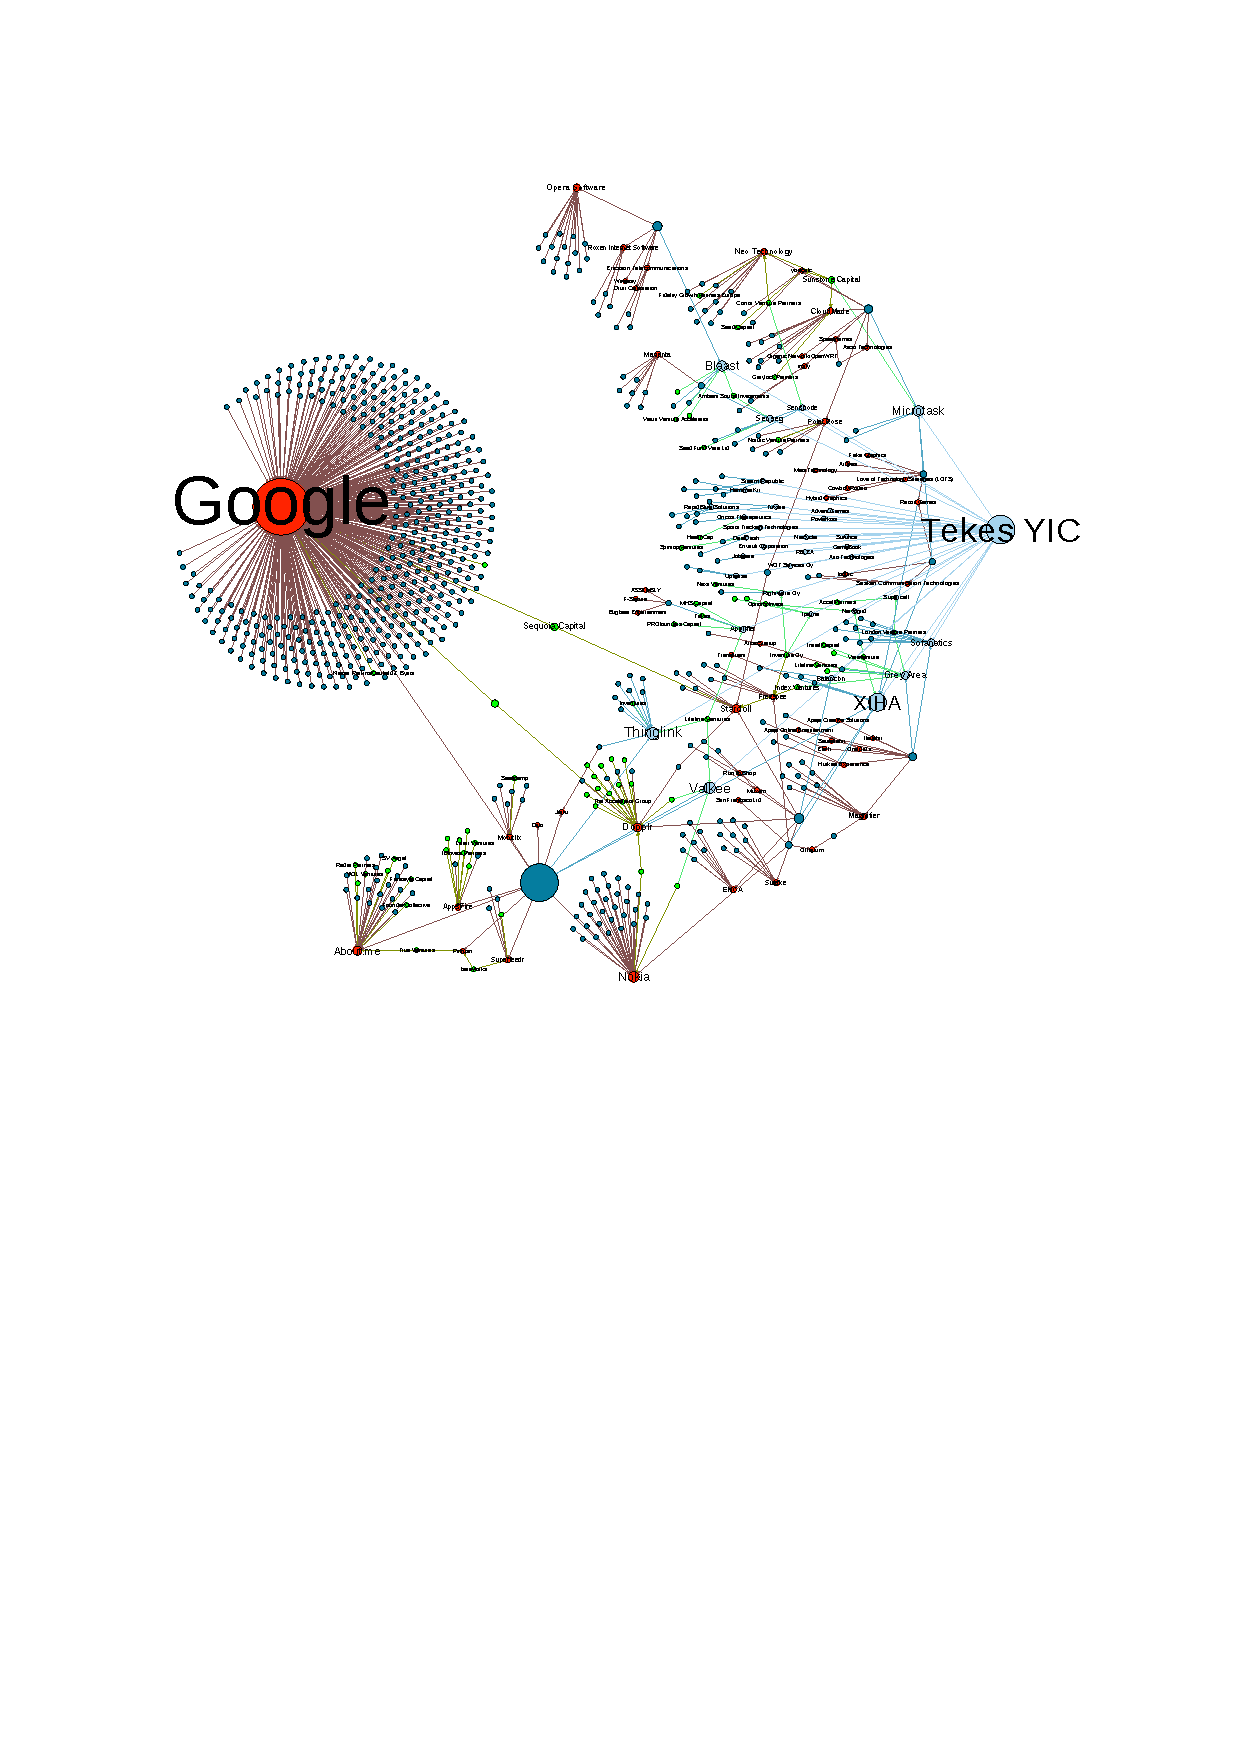
\includegraphics[width=12cm]{figure/Tekes-YIC-3-step.pdf}
\caption{Boundary specification: 3-step network visualization of Tekes Young Innovative Companies, their direct connections and the companies, investors and individuals that can be reached through the direct connections
 \citep{Huhtamaki2012NetworksFinland}}
\label{fig:tekes-yic-3-step}
\end{figure}

\begin{figure}[htb]
\centering
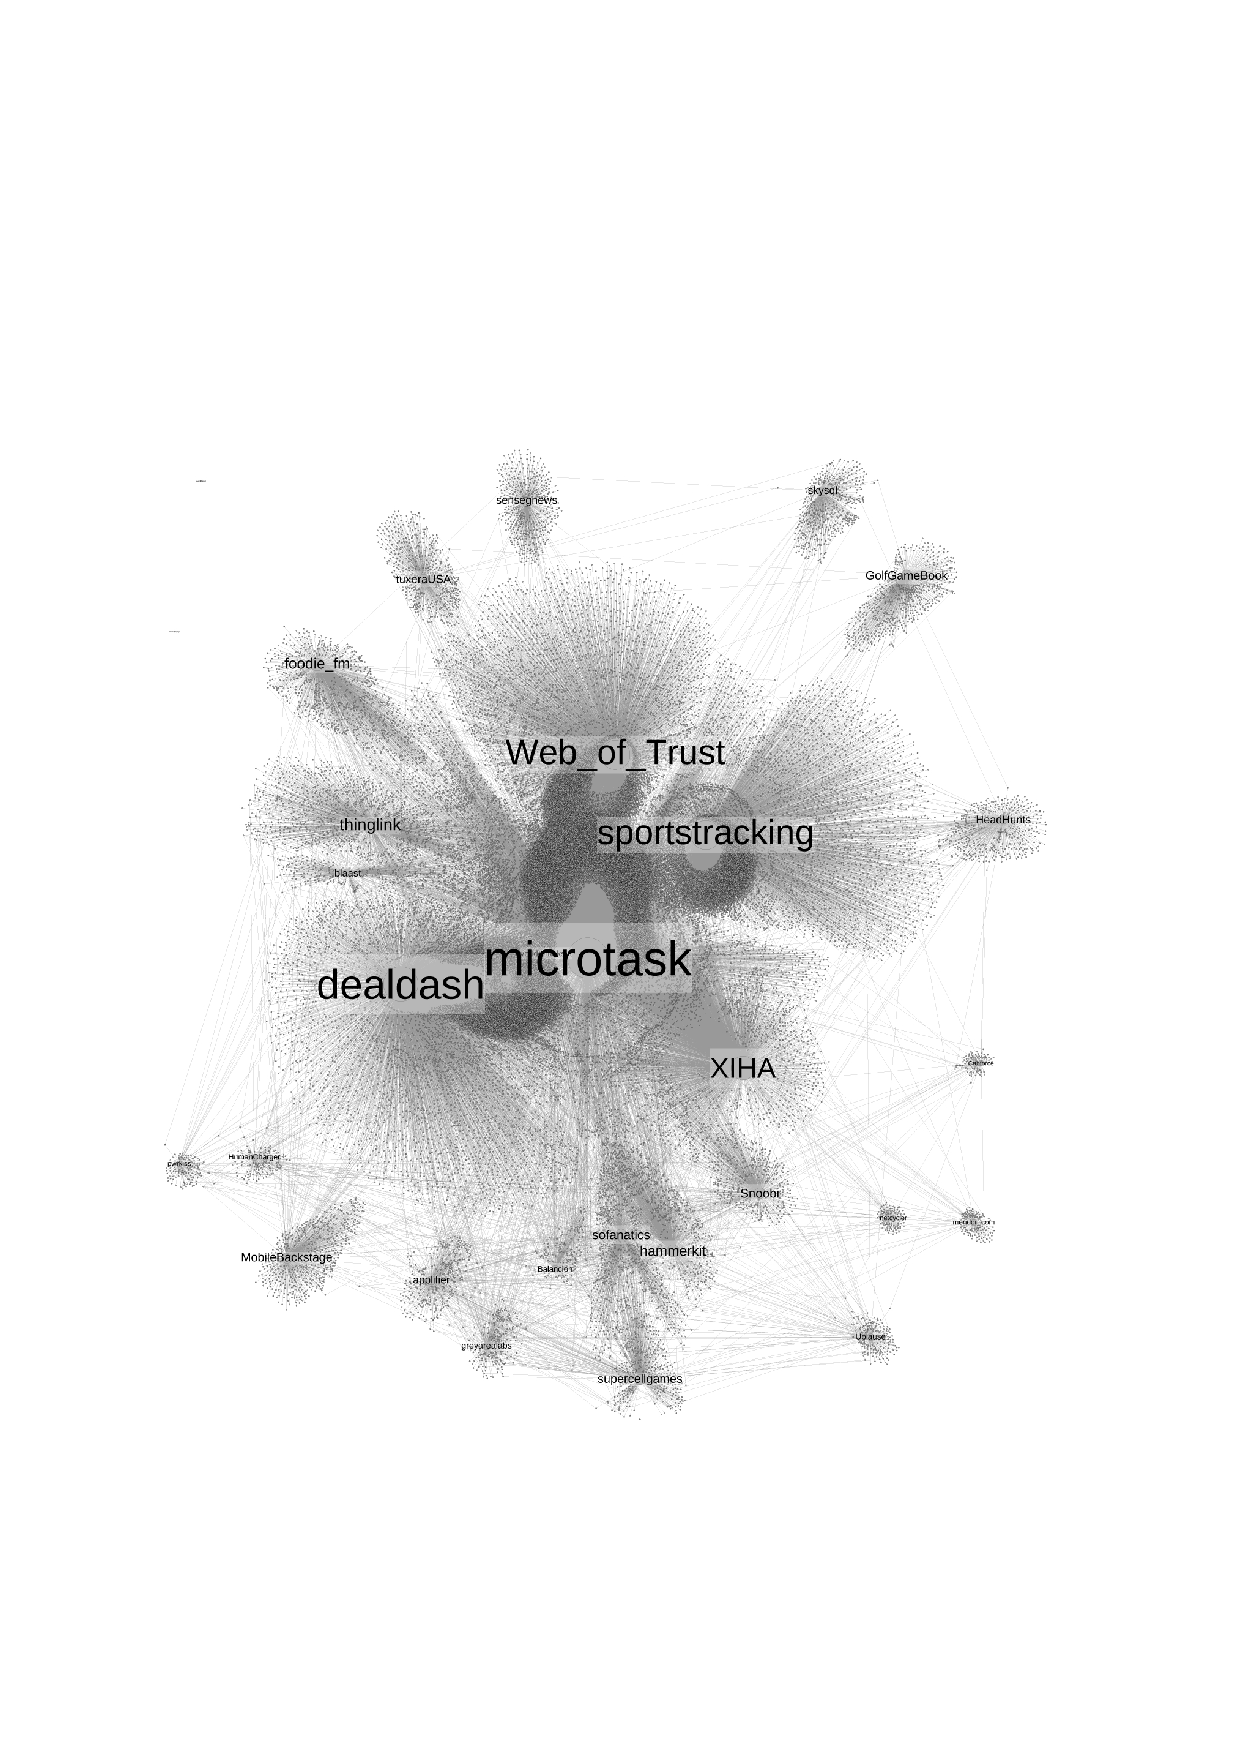
\includegraphics[width=12cm]{figure/Tekes-YIC-Twitter.pdf}
\caption{Social media analytics: 3-step network visualization of Tekes Young Innovative Companies, their direct connections and the companies, investors and individuals that can be reached through the direct connections
 \citep{Huhtamaki2012NetworksFinland}}
\label{fig:tekes-yic-twitter}
\end{figure}

In the Twitter network in Figure~\ref{fig:tekes-yic-twitter}, all the followers of a company are connected to the company with a directed edge pointing toward the company. The result is a two-mode or bipartite directed dichotomous network. Node size represents it indegree. Force-driven layout algorithm is used the lay out the Twitter network.

\subsection{Results and network-related insights}

The intestigative team joined with Tekes YIC program representatives for sensemaking to identify the key insights. With the first steps of connecting investors and individuals, it becomes evident that the companies selected individually into the Tekes YIC program are not without interconnections. When adding another step, the companies connected to the YIC program indirectly through investors or individual people are included and additional connecting tissue is introduced. Both Google and Nokia get pulled in through second-step connections and a single individual becomes a bridge between Nokia and Google and therefore has the largest betweenness value.

With ground truth, we know that an early social media platform Jaiku is one of the key individual developments in the Finnish Innovation Ecosystem. After Google acquired Jaiku, its founders Jyri Engeström and Petteri Koponen continued their ventures, Engeström as a serial entrepreneur in San Francisco Bay Area and Petteri Koponen through  Lifelines Ventures he co-founded. Interestingly, Lifeline Ventures is one of the early investors into Supercell, the most recent success story of the Finnish innovation ecosystem. More recently, Supercell CEO Ilkka Paananen joined the advisors of Lifeline Ventures to support the creation and growth of new startups.

Microtask, Web of Trust, Sportstracking and DealDash form the core of the Tekes YIC startup follower network. Microtask leads the charts with more than 30,000 followers followed by DealDash and Web of Trust. Supercell (\href{https://twitter.com/supercellgames}{@supercellgames}) has less than 1000 followers during the time of the investigation. In May 2016, more than 280,000 Twitter users follow Supercell.

\section{National level: Finnish Innovation Ecosystem}

Finnish Innovation Ecosystem is investigated in two consecutive experiments presented in \ref{pub:finland} and \ref{pub:multiscopicfinland}. Out of all the experiments included in this dissertation, \ref{pub:finland} is the first we \citep{Huhtamaki2013AFinancing} conducted\footnote{The paper on the investigation was first presented in EBRF conference in 2010 and invited to be published in TIM Review, see \url{http://timreview.ca/article/424}, and was eventually selected to book Value Co-Creation: Best of TIM Review.}. Therefore, its main contribution is in serving as a stepping stone for further investigation. 

In \ref{pub:multiscopicfinland}, we \citep{Still2013NetworksFinland} take up a grand challenge to present a solution for modeling and visualizing the network structure of the innovation ecosystem of a single nation, here Finland. To create a system-level view on Finnish Innovation Ecosystem, we utilize three complementary sources of data, each representing different aspects of the ecosystem.

We resolve the limitations of the separate datasets by building multiscopic views into networks of innovation relationships, using separate datasets. Moreover, in order to create an system-level view into Finnish Innovation Ecosystem, we create an aggregated dataset by combining the three individual sets of data. We proceed to support the interpretation of these visualizations by explaining context with network metrics as well as other descriptions.

The two investigations on the Finnish Innovation Ecosystem are conducted in innovation research projects funded by Tekes innovation research. The investigative team conducted the investigations independently, however project steering group members representing Finnish innovation ecosystem stakeholders had a role in formulating the research questions guiding the studies.  

\subsection{Rationale for network analytics}

Investigation of the Finnish Innovation Ecosystem is an attempt to utilize the potential of the data-driven approach to network analytics in the level of a national ecosystem. It stems from the observation  that traditional ways to measure innovation inputs and outputs are often industry-level aggregates and therefore do not allow for system-level insights on the innovation ecosystem under investigation \citep{Still2012ParadigmDigital}. Network representation of a national innovation ecosystem allows for observing e.g. the role of individual investors and patterns of acquisition and workforce flow and, in addition, developing a context for measurements and tailored action. More importantly, ecosystem-level view enables co-referencing and therefore more explicit support for sensemaking and attempts to form shared vision in between ecosystem stakeholders \citep{Russell2011TransformingOrchestration}. To recap, the presented multiscopic views into the Finnish Innovation Ecosystem allows for examining the relationships supporting value co-creation at various levels of the ecosystem as well as between those levels, providing novel possibilities for network orchestration and innovation management.

\subsection{Data sources}

Three complementary sets of data are used in the investigation. Thomson Reuters SDC includes in particular connections in between large, already established companies. In addition, to enable the investigation of the relationships around startups and growth companies, we use IEN Startup and IEN Growth to complement the analysis. More specifically, IEN Startup is used to create the microscopic view, IEN Growth the mesoscopic view and Thomson Reuters SDC the macroscopic view.

In addition to using the three sources of data in parallel, an aggregate dataset is created. The three datasets in use in the investigation are complementary and, at the same time, partly overlapping, therefore necessitating a refinement and curation process similar to what is being applied e.g. in data journalism \citep[cf.][]{2012DataHandbook} when creating the aggregated dataset.

\subsection{Network modeling decisions}
\begin{figure}[htb]
\centering
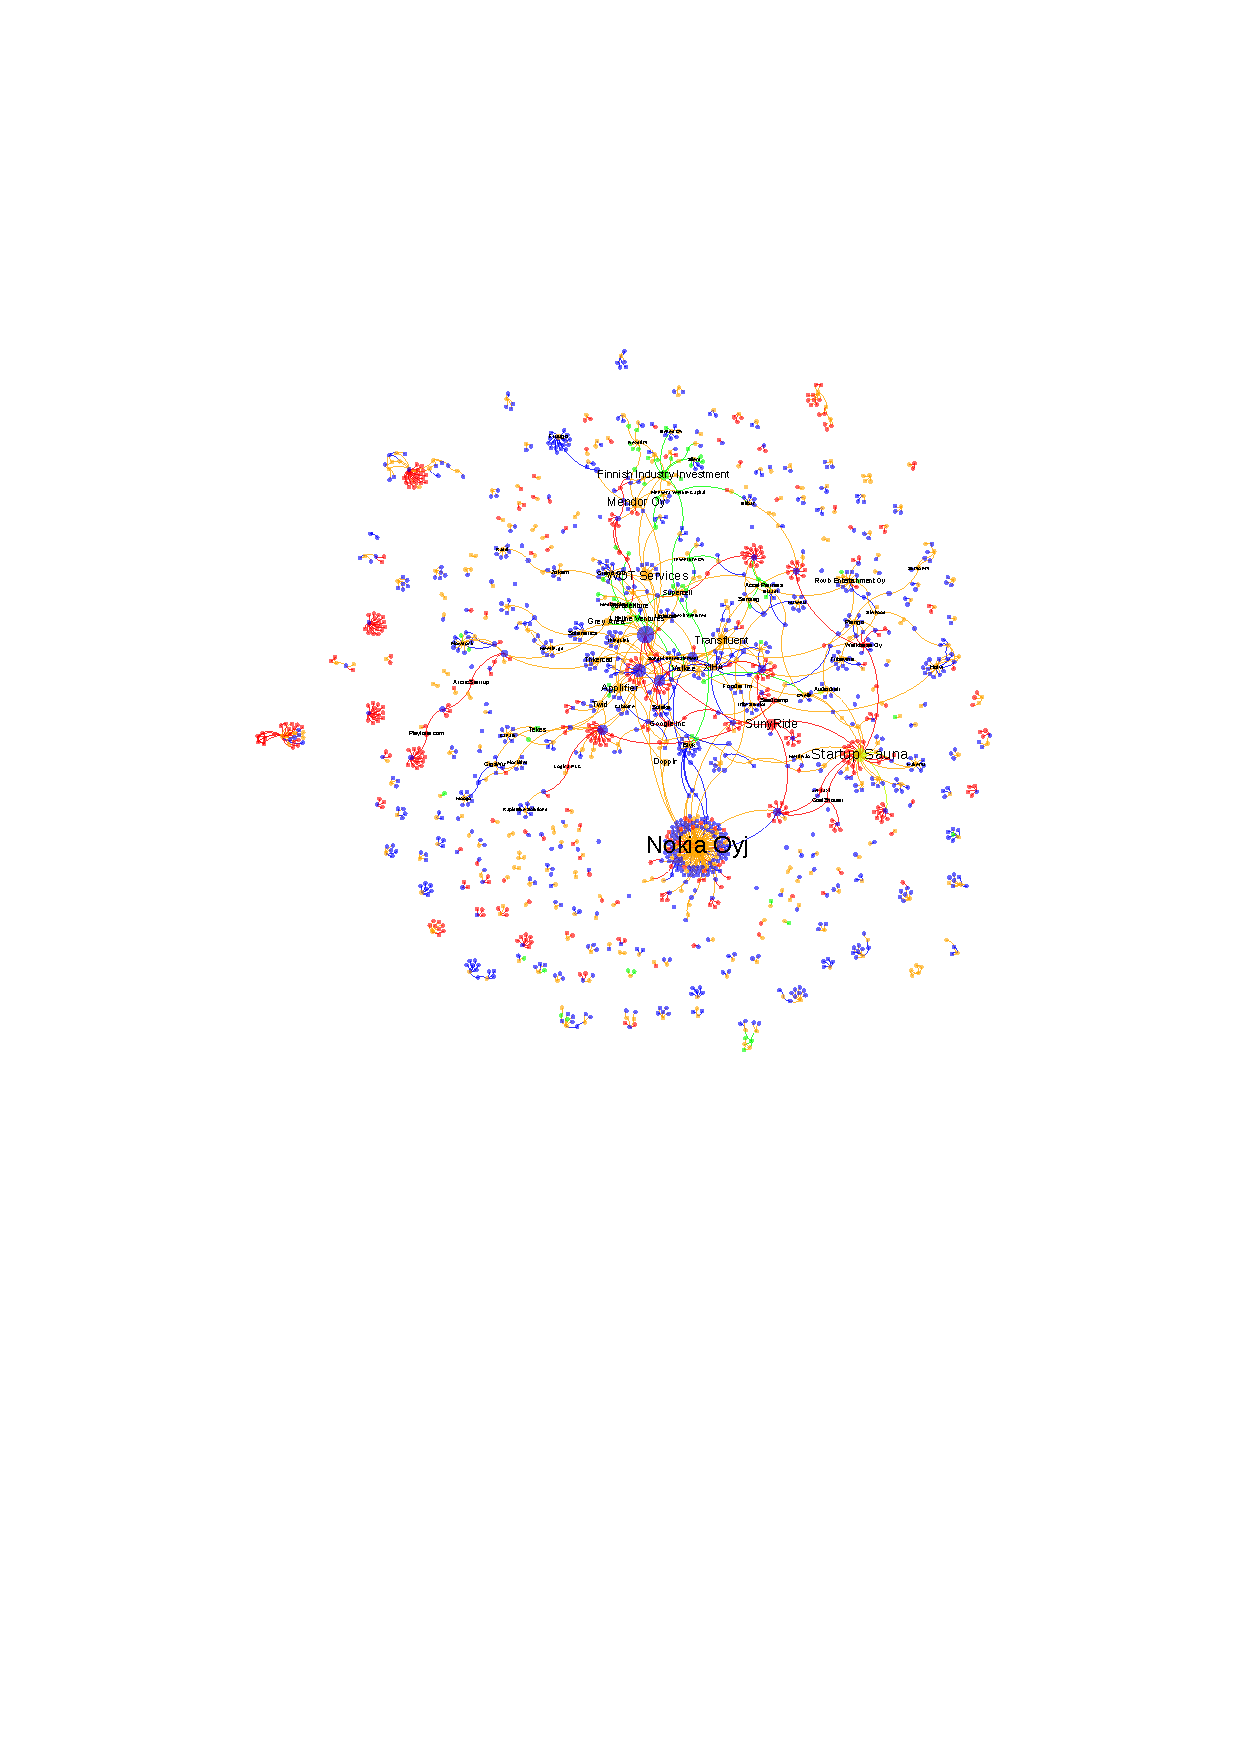
\includegraphics[]{figure/Finland-Multiscopic.pdf}
\caption{Data aggregation: Aggregate view to the Finnish Innovation Ecosystem using data on deals and alliances, executives and finance, and business angels and startups  
\citep{Still2013NetworksFinland}}
\label{fig:finland-multiscopic}
\end{figure}

\ref{pub:multiscopicfinland} is the first investigation in which we provide a multiscopic view into an innovation ecosystem, in this case the Finnish innovation ecosystem. In all, four different views into the Finnish Innovation Ecosystem are created. Macroscopic view shows the connections in between already established enterprises. Finnish companies are included and connected to other companies, Finnish or foreign, through deals and alliances. Mesoscopic view is built around Finnish growth companies. All the organizational investors as well as key individuals affiliated with the companies are included and connected to the Finnish companies. Microscopic view includes Finnish startups as well as business angels and other seed level investors and individual people affiliated to the companies. Multiscopic view, an aggregate of the three levels, provides a holistic system-view into the Finnish innovation ecosystem. 

To complement the multiscopic views into the Finnish Innovation Ecosystem, a number of quantitative descriptions for the different network representations is included in the article. These include the number of nodes, number of connections, density and diameter. Moreover, we list the top 10 actors based on betweenness centrality and degree for each of the networks.

\subsection{Results and network-related insights}

The main results of the investigation is the multiscopic view into the Finnish Innovation Ecosystem in Figure \ref{fig:finland-multiscopic}. The aggregated network depicts an ecosystemic view of Finland in Figure \ref{fig:finland-multiscopic} as it combines the Finnish companies from the three separate datasets and shows their direct connections. Hence, for the first time, we can see a single network representation of an ecosystem of the founders and angels, executives and financing organizations, as well as companies from startups to established enterprises. Overall, key actor of the ecosystem with the highest betweenness centrality is not surprising: Nokia is the super-node due to its connecting role in the Finnish ecosystem. % Accordingly, the same companies, financing organizations and individuals that have been prominent in previous lists and visualizations are highly visible in this ecosystemic view. 
As the weight of micro and meso-level data is greater, the top ten list of actors in the multiscopic level on basis of both betweenness and degree includes a significant number of individuals. There are 7 shared nodes between micro and macro-level views; 184 between micro and meso-level views; 10 between meso and macro-level views; four nodes appear in all three views: Rovio Entertainment, F-Secure, Mendor and Nokia. A number of foreign companies are included in the network through second-step connections, e.g. through acquisitions, investors, or individuals affiliated with Finnish companies.

\section{International level: EIT ICT Labs}

The network structure of EIT ICT Labs innovation ecosystem is investigated in \ref{pub:eitictlabs} \citep{Still2014InsightsVisualisations}. EIT ICT Labs, rebranded as EIT Digital \footnote{EIT ICT Labs becomes EIT Digital, \url{https://www.eitdigital.eu/news-events/news/article/eit-ict-labs-becomes-eit-digital/}} in June 2015, is a ``Leading European open innovation organisation.'' 

The investigation presented in \ref{pub:eitictlabs} builds heavily on \cite{Still2012ParadigmDigital} with an objective to explore opportunities for supporting the orchestration of innovation ecosystems, hence contributing to a fundamental capability in the networked world. We use a data-driven, relationship-based and network centric approach to operationalize Innovation Ecosystems Transformation Framework (IETF) \citep{Russell2011TransformingOrchestration} and present analysis, evaluation and interpretation in order to provide decision support and insights for transforming innovation ecosystems.

The investigative team joined with representatives of EIT ICT Labs Helsinki co-location center to conduct the two investigations \citep{Still2012ParadigmDigital, Still2014InsightsVisualisations}. In addition to mapping the network structure of EIT ICT Labs, the investigative team took up a scenario planning experiment that emerged trough interaction with EIT ICT Labs representatives to as a what-if question: What if San Francisco Bay Area was the seventh node of EIT ICT Labs? 

\subsection{Rationale for network analytics}

We investigate how data-driven network visualizations can be used to produce insights that support innovation ecosystem orchestration. The goal of network orchestration is a guided transformation of the ecosystem with continuous co-creation that allows the evolution of the processes needed to motivate and realize the transformation \citep{Russell2011TransformingOrchestration}. This process evolution accommodates the complex influences on innovation in a networked world and energizes innovation processes and outcomes. Through the lens of the IETF, a shared vision of the transformational potential of a dynamic innovation ecosystem is created through changes in actors, the events that they enable and the coalitions reflected in their relationships.

\subsection{Data sources}

After experimenting with in-house data on EIT ICT Labs activities, the investigative team together with EIT ICT Labs representatives decided to use IEN Dataset instead. The use of an external data source enables the  exploration of existing pathways in between the EIT ICT Labs co-location cities previously unknown to EIT ICT Labs operating team.

Innovation Ecosystem Network Dataset \citep{Rubens2010LeveragingMoves} is used as the sole data source. The dataset for the EIT ICT Labs sample is drawn by selecting all the companies that have their primary office in one of the six co-location cities of EIT ICT Labs: Berlin, Eindhoven, Helsinki, Paris, Stockholm, and Trento. In addition, to collect data representing companies and related individuals and investors in the SF Bay area, we listed all the key cities located in Silicon Valley area and complemented the list with San Francisco (including e.g. Berkeley).

\subsection{Network modeling decisions}

\begin{figure}[htb]
\centering
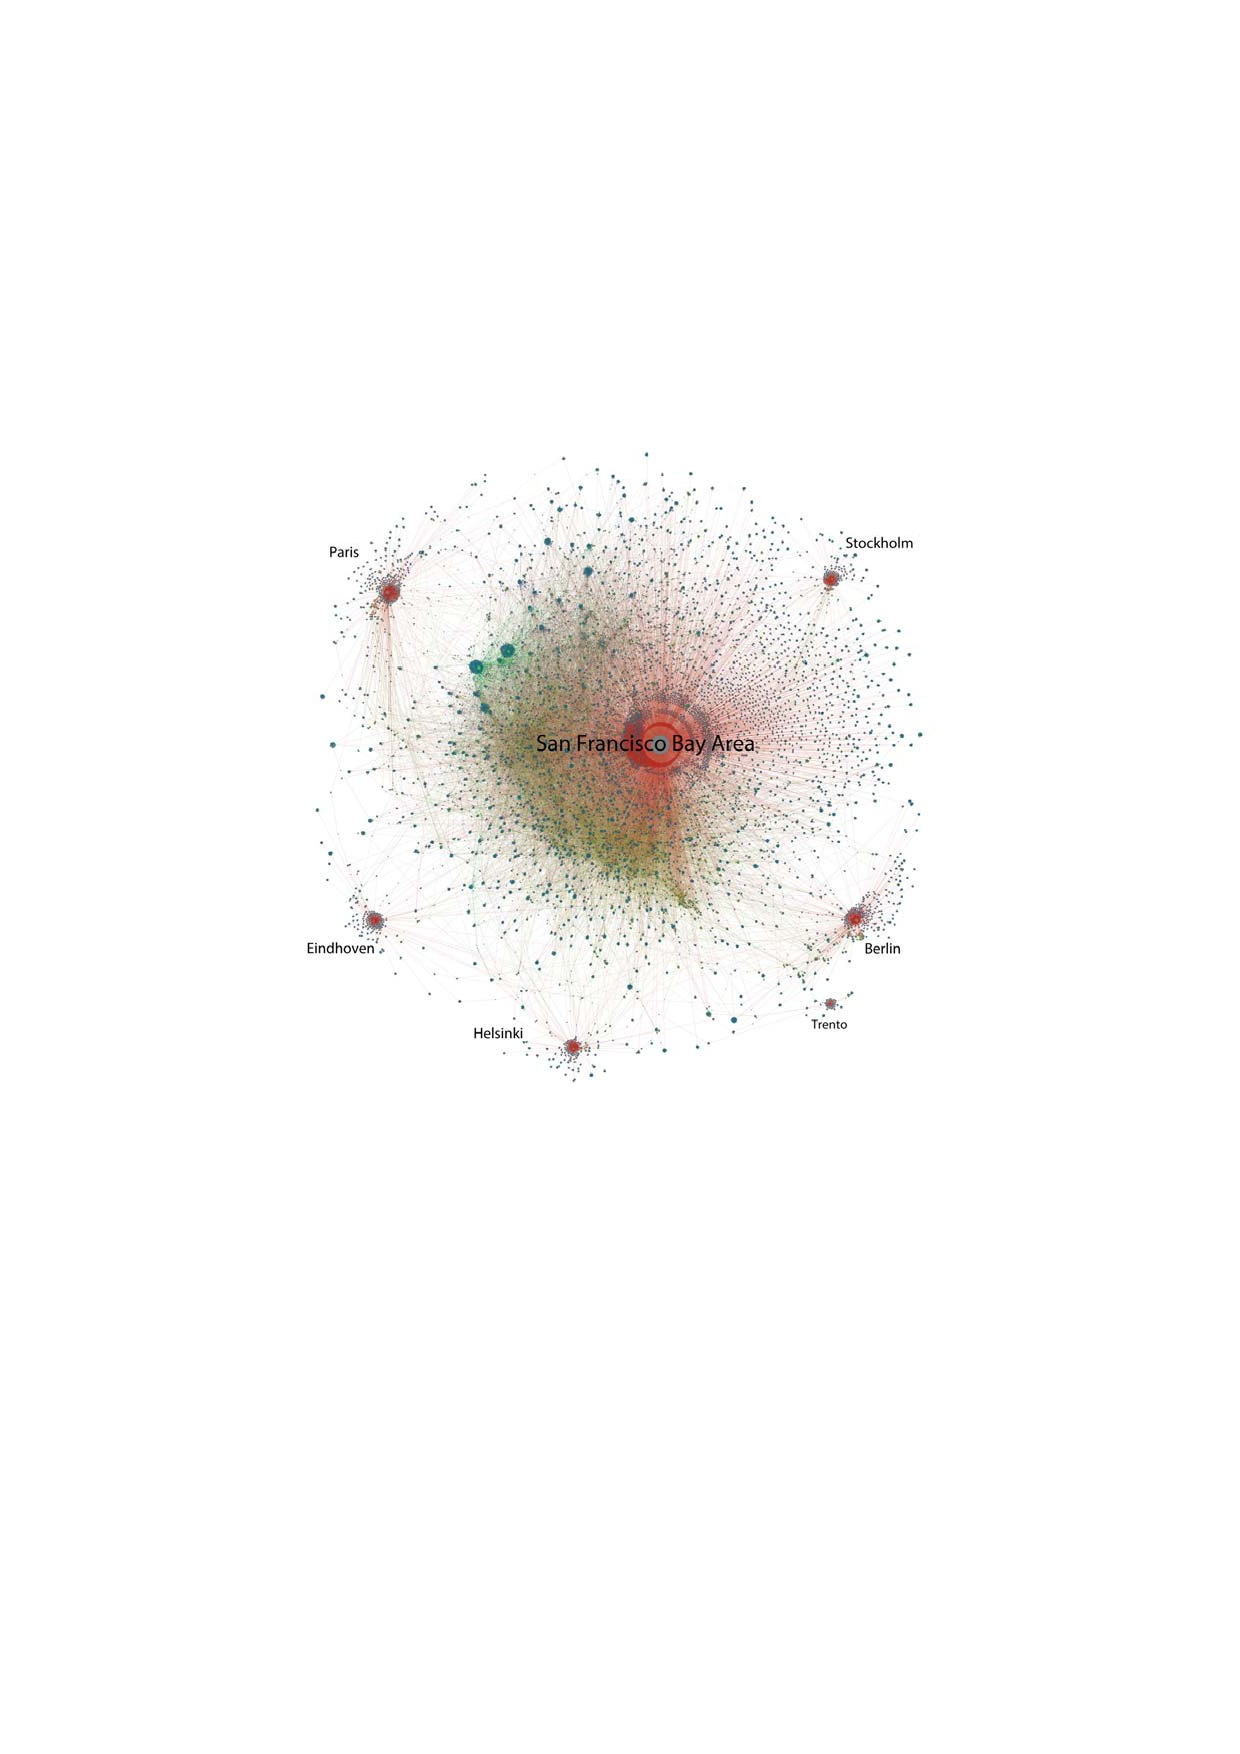
\includegraphics[width=0.925\textwidth]{figure/EIT-ICT-Labs-What-if-SF-Bay.pdf}
\caption{Scenario planning: What if San Francisco Bay Area was the 7th EIT ICT Labs co-location city \citep{Still2014InsightsVisualisations}}
\label{fig:eit-ict-labs-SF-Bay}
\end{figure}

The six co-location cities, Paris, Berlin, Stockholm, Helsinki, Eindhoven, and Trento, form the core of the network. Each company in the sample is connected to the city in which its primary office is located. All key individuals (founders, board members and C-level executives) in the dataset affiliated with one or more of the companies in the sample are connected to the companies. Next, financial organizations identified with funding events for those companies are added as nodes and connected to respective companies. 

Metrics used in the analysis include the number of each type of actors and the changes in the values over years 2011, 2012, and 2013. Moreover, we measure the degree and betweenness of the six co-location cities and the change in the values between 2012 and 2013 to investigate the changes in the relative position of the co-location cities.

\subsection{Results and network-related insights}

The results of the investigation include changes in the numbers of actors connected individual co-location cities compared to our previous investigations and a set of visualizations on the structure of the EIT ICT Labs ecosystems. Moreover, the role of individuals and investors in building interconnections between EIT ICT Labs co-location cities is shown. 

The prominent role of investors as the connecting tissue between the individual co-location cities is a key result of the investigation. Moreover, the realization that many of these investors are, in fact, based in Silicon Valley led us, in collaboration with EIT ICT Labs representatives, to ask a key what-if question: What if San Francisco Bay Area was the 7th EIT ICT Labs co-location city? Figure \ref{fig:eit-ict-labs-SF-Bay} shows that when San Francisco Bay Area is added as the 7th co-location city and the network representation is laid out with force-driven algorithm, San Francisco Bay Area becomes the focal point of the network through which most of the connections between the current co-location cities go through. With San Francisco Bay Area, the amount of nodes increases from 6,187 to 35,389 and edges from 7,050 to 51,106.

\section{Summarizing the investigations}

We will conclude this chapter with a summary of the results and network related insights into the investigated innovation ecosystems. Finally, we will discuss the utility and added value of the investigations.

For the investigation on Demola, we joined with the Demola operating team to explore ways to apply data-driven visual network analytics in representing the structure and dynamics of an ecosystem engager that is targeting to facilitate collaboration between (Tampere-based) universities and companies. In collaboration, i.e. through the process of guided emergence, we found an animation of the evolution of the network structure of Demola platform to be particularly useful in presenting, describing, promoting, and marketing the platform for existing and new stakeholders.

In the investigation on Tekes Young Innovative Companies, we explored the interconnections in between companies taking part in the YIC program. Two sources of data were used to conduct the study, Innovation Ecosystem Network Dataset and Twitter. We show that connections exist in between the companies that are individually selected into the YIC program. These interconnections are key in revealing the innovation ecosystem that Tekes is interacting with through their support for individual companies. Moreover, the investigation makes a contribution with an example of using social media data to give a system-level view into those interested in the companies. On a longer term, should the Tekes YIC program be successful in selecting and supporting companies in growing, we would see a food chain of investors and acquirers emerge. Business angels, serial entrepreneurs--either active or successful--would also take a central role in such a network representation of the innovation ecosystem around the YIC program. 

In the investigation of the Finnish Innovation Ecosystem, we provided a system-level view into a national innovation ecosystem. The ecosystem representation includes established enterprises, growth companies, and startups as well as investors and key individual affiliated with the companies. More specifically, we create four different representations of the ecosystem, microscopic, microscopic, macroscopic and multiscopic. A handful of key individuals that entered the global startup ecosystem early and were successful in growing and selling a company maintain a prominent role in the Finnish Innovation Ecosystem. Nokia is visible through its role as a source of talent flowing into the ecosystem. Startup Sauna, a student-driven accelerator\footnote{Startup Sauna accelerator is ``Building a better startup ecosystem one company at a time'', \url{http://startupsauna.com/}},  also has a notable role. Recent success stories Rovio Entertainment and Supercell take a peripheral position; the presented approach does, however, enable monitoring the evolution of the ecosystem around them in the future. Our practical suggestions for startups include active communication and data sharing using a wide variety of media and, particularly for policy makers, the utilization of network views for targeted actions as well as for creating shared understanding and vision.

From network orchestration viewpoint, in collaboration with EIT ICT Labs representatives, our results indicate that with coordinated and continuously improved use of visual and quantitative social network analysis, special characteristics, significant actors and connections in the innovation ecosystem can be revealed to develop novel insights. Creating a network representation of EIT ICT Labs including San Francisco Bay Area as the 7th node is an example of scenario planning that the approach proposed in this dissertation enables. We conclude that the IETF transformation framework can be used to develop shared vision and to support the orchestration of innovation ecosystem transformations.

\section{Utility and added value of the investigations}

In summarizing the approach and key findings of our first investigation on EIT ICT Labs \citep{Still2011ExplainingEurope}, \cite{Turpeinen2011}, EIT ICT Labs Helsinki co-location lead at the time and our collaborator in the investigation, pointed out the key role of mobility in EIT ICT Labs' attempt to turn Europe into an equal competitor to Silicon Valley. While EIT ICT Labs' key way to support mobility was at the time the European-level master school, the network representation of the interconnections between EIT ITC Labs co-location cities provided an interesting insight: the role of individual universities and in particular venture capital investors in bridging the co-location cities is very important. When revisiting investigation on EIT ICT Labs \citep{Still2012ParadigmDigital, Still2014InsightsVisualisations}, we joined with EIT ICT Labs representatives to ask a what-if question, something that is seen integral in scenario planning \citep{Schoemaker1995ScenarioThinking}.

In light of our investigations, we were exited to witness the news of, first, EIT ICT Labs opening up an office in San Francisco for ``Building a bridge between the European ecosystem and the San Francisco Bay Area''\footnote{EIT ICT Labs opens new Silicon Valley Hub, \url{http://eit.europa.eu/newsroom/eit-ict-labs-opens-new-silicon-valley-hub}} and, second, Marko Turpeinen appointed to lead the Silicon Valley Hub\footnote{Marko Turpeinen to lead EIT ICT Labs Silicon Valley Hub,  \url{http://www.aalto.fi/en/current/news/2015-04-29-002/}}. While the specifics of the decision-making process related to these two events remain unknown to us, we argue that the process related to the what if-scenario as well as the exploration of the structure of the existingecosystem in general contributed and supported discussions and decision-making related to  EIT ICT Labs' presence in Silicon Valley.

The Demola investigation was conducted during the time when the Demola concept was only beginning to grow outside Tampere and Finland. Similarly to the investigation on EIT ICT Labs, our co-creators in the Demola investigation knew the Demola operations by heart and therefore saw no value in exploring the structure of the Demola network for supporting their internal operations and decision-making. Instead, using network visualization and particularly the animation of the evolution of Demola platform as a network was perceived very valuable in presenting, describing, promoting, and marketing the platform concept to existing and new stakeholders. 

Investigation of the Finnish Innovation Ecosystem \citep{Huhtamaki2010AFinancing} marks our first attempt to explore an innovation ecosystem with a data-driven visual network analytics approach, with the alumni network study \citep{Rubens2011AlumniAnalysis} serving as an example of the approach in a related context. The follow-up study in \ref{pub:multiscopicfinland} is the first in which we used several sets of data both in parallel as well as in creating an aggregated dataset and a respective view into an innovation ecosystem. In all, the two investigations on the Finnish innovation ecosystem have supported introducing and experimenting with new features into the research process following the data-driven visual network analytics approach.

All of the investigations included in this dissertation are conducted in Tekes-sponsored innovation research projects. Innovation ecosystem orchestrators and policy makers have joined the project both to provide context for the investigations as well as members of project steering groups. We have witnessed the applications of the presented approach being introduced into strategic foresight and impact assessment activities both within Tekes programs as well as e.g. in Council of Tampere Region.
\chapter{Design principles for analyzing innovation ecosystems as networks}
\label{ch:ecosystemnetworks}

After reviewing the individual investigations conducted in this dissertation, we use this chapter to make explicit the first set of Generalized Outcomes of the research \citep{Sein2011ActionResearch}, i.e. to synthesize the generalized outcomes of the experiments for developing guidelines for modeling and analyzing innovation ecosystems as networks. This contributes to \ref{objective:ecosystemnetworks} of the dissertation.

For an overview of how the individual experiments contribute to the overall action design research process, we will start the chapter with placing the experiments to a diagram on ADR Stages and Principles \citep{Sein2011ActionResearch}. Figure~\ref{fig:adrapplied} recaps the key principles of ADR in the context of this dissertation.

% Original diagram: https://docs.google.com/presentation/d/1lRsPTkR5w9uXl0sqO-0p1UN8D48b9Lb1cZZMzWT4OqQ/edit?usp=sharing
\begin{figure}[htb]
\centering
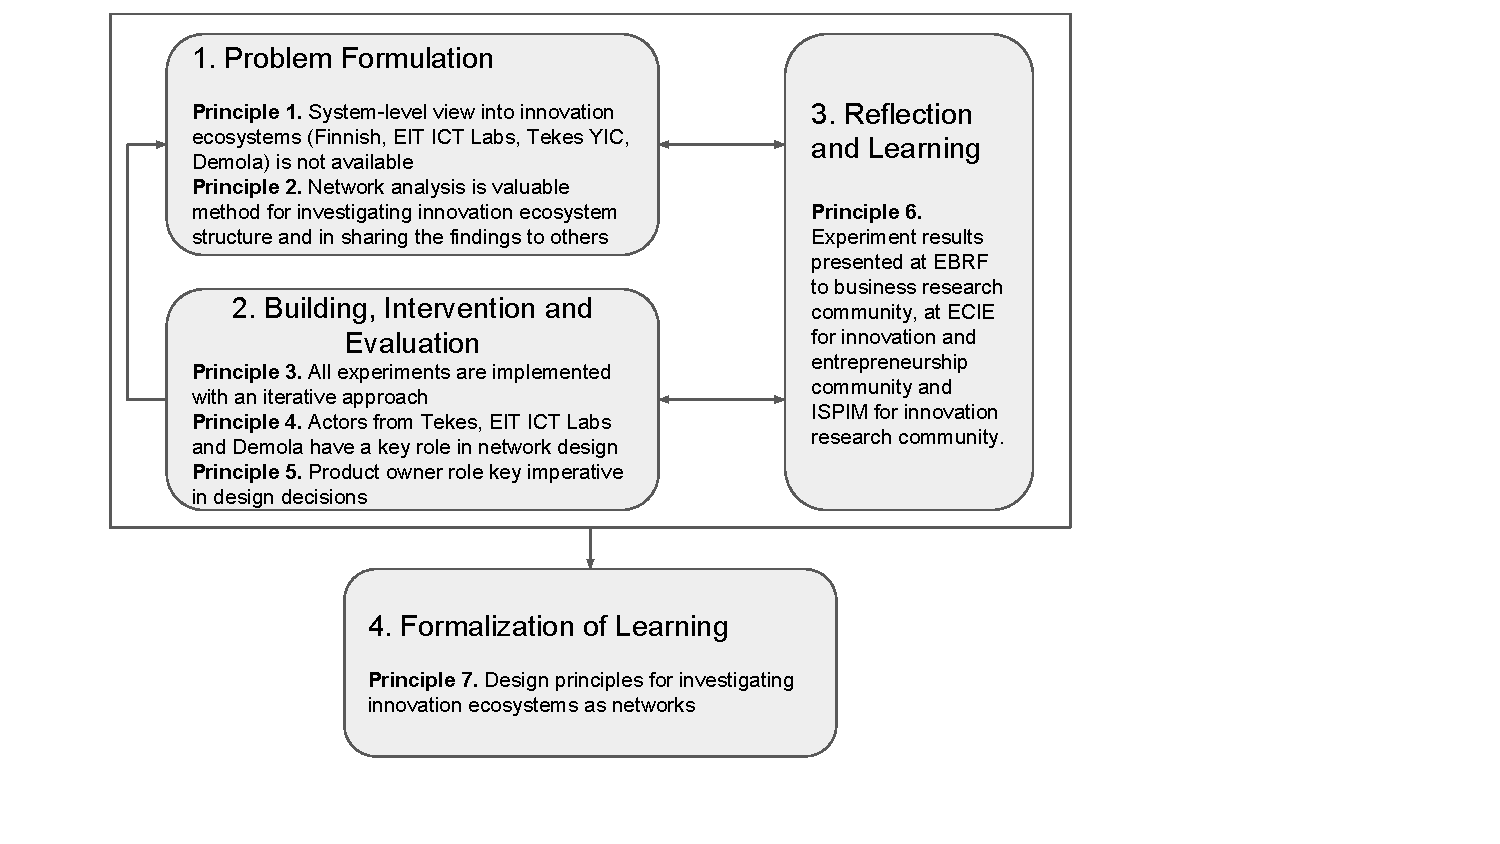
\includegraphics[width=11cm]{diagram/ADR-innovation-ecosystems-as-networks.pdf}
\caption{Action Design Research for investigating innovation ecosystems as networks \citep[following][]{Sein2011ActionResearch}\label{fig:adrapplied}}
\label{fig:ADR-innovation-ecosystems-as-networks}
\end{figure}

\section{Data for network analysis}
\label{sec:networkdata}

The experiments included in this dissertation are based on two main sources of data, the Innovation Ecosystems Network Dataset \citep{Rubens2010LeveragingMoves} and Thomson Reuters SDC. Thomson Reuters SDC is one of the most prominent sources of inter-firm relationships \citep{Schilling2009}. Thomson Reuters SDC is a prime example of a traditional company data sources from which start-ups and growth companies are oftentimes missing. IEN Dataset provides socially curated (or crowd-sourced) rich data about startup and growth companies in almost real-time, though with a public bias. In concert, the two sources of data provide means for creating several complementing views into innovation ecosystems. Following \ref{pub:multiscopicfinland}, the datasets represent different levels of the innovation ecosystem and therefore enable the creation of both microscopic, mesoscopic, macroscopic as well as multiscopic views into the innovation ecosystem \citep{Still2013NetworksFinland}.

More specifically, IEN Dataset includes two subsets of data, Startups and Angels for a microscopic view and Executives and Finance for a mesoscopic view. In addition, Thomson Reuters SDC can be used for data on Deals and Alliances between major enterprises forming the core of the existing business ecosystem, i.e. the macroscopic view. The established enterprises acquire companies and act as sources of talent for startups and growth companies and it is therefore often important to include them in the network representations.

Investigation of the Finnish Innovation Ecosystem in \ref{pub:multiscopicfinland} is the first in which we create an aggregate set of data by combining the three different sets through actors that appear in more than one dataset. With the aggregated dataset, we provide a system-level view into the Finnish Innovation Ecosystem. In our investigations, we use a semi-manual process to aggregate the datasets and call for means to fully automate the process by applying string matching \citep{Navarro2001AMatching} and named entity recognition \citep{Finkel2005IncorporatingSampling}.

In \ref{pub:tekesyic}, we further use social media data from Twitter to investigate the structure and interconnections of the Twitter followers of the startups in Tekes Young Innovative Companies program. The list of companies in the program is scraped from Tekes website and Twitter usernames are collected manually. In \ref{pub:finland}, two complementing sources of data are in use: the member list of Finnish Venture Capital Association\footnote{Members of the FVCA, \url{http://www.fvca.fi/en/members}} and ArcticIndex\footnote{ArcticIndex is no longer active. It Was maintained by ArcticStartup, \url{http://arcticstartup.com/}}, a socially constructed dataset of Nordic and Baltic startups.

All of the aforementioned datasets originate from publicly available sources. Moreover, proprietary in-house data can be used to represent and analyze innovation ecosystems as networks. Investigation of the Demola platform in \ref{pub:demola} is fully based on in-house data. The first attempt to create a network representation of EIT ICT Labs innovation ecosystem was based on their in-house data. We soon realized, however, that through day-to-day operations, EIT ICT Labs actors know the structure emerging from the in house data by heart. Therefore, we instead decided to use IEN Dataset to investigate the already existing connections in between the then six co-location cities for insight on the latent social structure of the ecosystem as well as  mobility patterns within the co-location cities.

Table~\ref{tab:networkdata} presents a summary of the data sources used in each investigation.

\begingroup
\captionof{table}{Details on collecting and processing data for the investigations}\label{tab:networkdata}
\begin{tabular}{p{2cm} p{3cm} p{4cm} p{3cm}}
\toprule
Experiment & Source & Collecting & Refinement \\
\midrule

Demola &
Project database internal to Demola &
Tailored script for exporting the data from database in use in Drupal CMS &
Unifying project category names \\

Mobile ecosystem &
Innovation Ecosystems Network Dataset (IEND), Thomson Reuters SDC (TR SDC) &
Tailored script that traverses a NoSQL implementation of IEND proxy, TR SDC data imported as an Excel spreadsheet &
Done as part of IEND and Thomson Reuters SDC curation \\

Tekes Young Innovative Companies &
IEND, Twitter &
Tailored scripts for traversing a NoSQL implementation of IEND proxy and accessing Twitter data through a REST API &
Done as part of IEND curation \\

Finnish innovation ecosystem I & 
IEND & 
Tailored script that traverses a NoSQL implementation of IEND proxy &
Done as part of IEND curation \\

Finnish Innovation Ecosystem II  &
IEND, TR SDC &
Tailored script that traverses a NoSQL implementation of IEND proxy, TR SDC data imported as an Excel spreadsheet &
Connecting companies across individual datasets through the creation of unified names \\

EIT ICT Labs &
IEND &
Tailored script that traverses a NoSQL implementation of IEND proxy &
 Done as part of IEND curation \\
\bottomrule
\end{tabular}
\endgroup

\section{Representing innovation ecosystems as networks}
\label{sec:networkrepresentation}

Visual analytics is a key source for requirements in designing the principles for investigating innovation ecosystems as networks. Both in the investigations in which we interacted with innovation ecosystem stakeholders as well as in the investigations that the research team conducted independently, we ended up representing the innovation ecosystems under investigation as multimodal networks. Table~\ref{tab:networkdesign} recaps the network modeling decision in the individual investigations.

We do, however, realize that multimodal networks limit the possibilities for calculating node and network level metrics to quantify the structural properties of the network and the structural roles of the individual actors to be utilized e.g. in statistical analysis. At the same time, we observed in the investigations that using a one-mode network representation of an ecosystem reduces significantly the complexity of the innovation ecosystem under investigation and therefore reduces transparency. Moreover, one-mode network representation does not allow for truly system-level insights of the structural patterns of the innovation ecosystem. The use of one-mode and multimodal networks in concert to support processes that iterate between exploration and specific measurement insists on future development and experimentation. 



\begingroup
\captionof{table}{Network design details for experiments}\label{tab:networkdesign}
\begin{tabular}{p{3cm} p{4cm} p{5cm}}
\toprule
Experiment & Boundary specification & Network modeling \\
\midrule

Demola &
Include the whole project database &
Multimodal network of universities, projects and companies. Connections are formed through project affiliation \\

Mobile ecosystem &
Start from pairs of companies, include their first and second tier connections &
One-mode networks for Thomson Reuters SDC, multimodal networks for IEND \\

Tekes Young Innovative Companies &
Start from companies in Tekes YIC program, include their first and second tier connections &
Multimodal network of companies, key individuals and investors \\

Finnish innovation ecosystem I & 
Start from companies in Finland, include their first tier connections & 
Multimodal network of companies, key individuals and investors \\

Finnish innovation ecosystem II &
Start from companies in Finland, include their first tier connections &
Microscopic, mesoscopic, macroscopic and multiscopic view to Finnish Innovation ecosystem. Macroscopic view is non-directed one mode network, the others are non-directed multimodal networks \\

EIT ICT Labs &
Start from the six EIT ICT Labs co-location cities, include companies having their primary office in one of the cities, include individuals and investors connected to the companies &
Multimodal network of companies, key individuals and investors \\
\bottomrule
\end{tabular}
\endgroup

\section{Analyzing innovation ecosystems as networks}

Network analysis allows for measuring and analyzing the structural properties of innovation ecosystems in all three levels of analysis, i.e. in system, relationship, and actor level \citep{Jarvi2016TakingReview}. In system-level, network metrics include density, diameter, and clustering coefficient. Edge weight is a key metric in relationship level and, in addition, detailed relationship properties can be included in network data and used in the analysis of dyads, i.e. pairs of nodes. Node degree, indegree, outdegree and betweenness are examples of node-level metrics.

Table~\ref{tab:networkanalysis} summarizes the network and node-level metrics we apply in the different experiments. Visual analytics has a focal role in this dissertation and therefore the network metrics serve primarily in highlighting actors in significant roles in an innovation ecosystem. Betweenness centrality is the most used node-level metric. Edge weight is used throughout the investigations. Network metrics allow for comparing the structural properties of individual innovation ecosystems to each other. In this dissertation, network metrics describe the structure of innovation ecosystem and, moreover, in the the mobile ecosystem investigation network metrics are used to compare ecosystems with each other.

\begingroup
\captionof{table}{Network design details for experiments}\label{tab:networkanalysis}
\begin{tabular}{p{2.5cm} p{2.5cm} p{3cm} p{3.75cm}}
\toprule
Experiment & Network metrics & Edge metrics & Node metrics \\
\midrule
Demola &
Not applied &
Weight for the number of students representing a university & 
Betweenness for node's ``connecting role in the network'' \\

Mobile Ecosystem & 
Size, diameter, clustering, density &
Weight for the number of deals and alliances between companies &
Degree, betweenness, clustering coefficient \\

Tekes Young Innovative Companies &
Size &
Dichotomous weight &
Betweenness to ``to highlight the individuals, companies and investors that have an important connecting role in the network'' \\

Finnish Innovation Ecosystem I & 
Size & 
Dichotomous weight &
Degree, betweenness \\

Finnish Innovation Ecosystem II  &
Size, number of edges, density, diameter &
Dichotomous weight &
Betweenness \\

EIT ICT Labs &
Size, number of edges &
Dichotomous weight &
Degree, betweenness ``as a mobility factor to illuminate the potential of individual nodes to serve as bridges between the EIT ICT Labs co-locations'' \\
\bottomrule
\end{tabular}
\endgroup

\section{Visualizing innovation ecosystems as networks}

Visual network analysis is an organic part of the approach taken in this dissertation. To reiterate \cite{Freeman2000VisualizingNetworks}, visual network analysis allows for two important tasks in investigating a phenomenon:  first, it supports investigators in observing the social structures emergent in the empirical data representing a phenomenon under investigation for insights and, second, it provides a tool for sharing the findings to others with representations that support co-referencing and the emergence of a shared understanding.

Table~\ref{tab:networkvisualization} recaps the key visualization-related design decisions in the investigations. In all of the investigations, we have used a force-driven algorithm to lay out the nodes. More specifically, we have applied the two variants of Force Atlas algorithm implemented in Gephi \citep{Bastian2009Gephi:Networks}. A consistent color scheme for nodes was established already in the first investigation. The investigative team observed that using colors to identify node types--green for investors, red for companies and blue for individuals--over time eases the visual investigation of networks as observers become familiar with the meaning of the different colors. We further note that consistency of the network layout is an important objective in designing the analysis process when visual network analytics is used to investigate an innovation ecosystem over time. We will come back to this topic in the context of the Ostinato Model in Chapter~\ref{ch:ostinato}.

\begingroup
\captionof{table}{visualization details for the experiments}\label{tab:networkvisualization}
\begin{tabular}{p{3cm} p{3cm} p{6cm}}
\toprule
Experiment & Layout & Visual properties \\
\midrule
Finnish Innovation Ecosystem I & 
Force-driven & 
Node color represents its type: red for companies, green for investors and blue for individuals  \\
Mobile Ecosystem &
Force-driven &
Node color represents its type: red for companies, green for investors and blue for individuals  \\
Tekes Young Innovative Companies &
Force-driven &
Node color represents its type: red for companies, green for investors and blue for individuals  \\
Finnish Innovation Ecosystem II  &
Force-driven &
Node color represents its type: gold for Finnish companies, red for foreign companies, green for investors and blue for individuals  \\
Demola &
Force-driven, dynamic when animating network evolution &
For projects, node color represents its membership in network cluster; company nodes are represented in light green \\
EIT ICT Labs &
Force-driven &
Node color represents its type: red for companies, green for investors and blue for individuals  \\
\bottomrule
\end{tabular}
\endgroup

\section{Design guidelines for network representation and analysis}
\label{sec:designguidelines}

Through the experiments reviewed in Chapter~\ref{ch:experiments}, we have investigated a number of innovation ecosystems with the visual network analytics approach. Next, to generalize and make explicit the observations we have made through the experiments and to support future efforts to model and represent innovation ecosystems as networks to support their investigation, we conclude the chapter with a set of design guidelines stemming from the experiments to guide analysts and researchers in taking a data-driven visual network analytics approach to innovation ecosystem investigations.

\subsection{Modeling innovation ecosystems as networks}
The decisions done in network modeling depicts the options for using different node-level metrics in analysis. Directed one-mode network with weighted connections allows the use of the widest range of metrics. In all of the investigations included in this dissertation, however, together with several ensembles of investigators, we have decided to represent innovation ecosystems with multimodal networks.

\guideline{1a}{Companies, key individuals, and investors are the basic entities in innovation ecosystem network representations}

\guideline{1b}{Multimodal networks provide an intuitive starting point for representing innovation ecosystems as networks for a system-level view of its structure}

\guideline{1c}{One-mode networks enable detailed quantitative and statistical analysis with the expense of reducing the complexity of the ecosystem}

\guideline{1d} {Edge direction and weight introduce additional means to utilize network metrics in supporting the analysis}

\subsection{Analyzing the networks}

In visual analytics, network metrics are used to highlight actors in different structural positions in the network. Node degree, indegree and outdegree are the most simple metrics. Betweenness centrality is a useful metric also in the context of multimodal networks. \cite{Hansen2011AnalyzingWorld} refer to betweenness centrality as ``Bridge Scores for Boundary Spanners''. Moreover, additional network metrics become available when an innovation ecosystem is represented as a directed one-mode network. 

\guideline{2a}{Node degree identifies actors with the largest amount of connections}

\guideline {2b}{Outdegree identifies the most active actors}

\guideline {2c}{Indegree is the simplest metric for prestige or authority}

\guideline{2d}{Betweenness highlights nodes that have a bridging role in the network}

\subsection{Visualizing the networks}

We have applied force-driven layout in all of the investigations included in this dissertation. A key reason for this is that the core investigative team has remained the same throughout the investigations and have continued to use force-driven layout. Nevertheless, all the other stakeholders in the investigations have also found the basic principle behind the force-driven layout to be intuitive. To our experience, the force-driven layout allows for the visual identification of network clusters and actors bridging the clusters.

Visual consistency is important in supporting investigations where different network representation of the innovation ecosystem under investigation are created. We have established a consistent color scheme for innovation ecosystem actors. Even more important is to maintain the positions of the individual actors and clusters of actors in between different representations, snapshots and rounds of investigations. We discuss this in more detail when describing the Ostinato Model in Chapter~\ref{ch:ostinato}.

Filtering is a key approach in reducing the complexity of the visual representations of innovation ecosystem networks. At best, an  investigator analyzing the network representation of an innovation ecosystem is able to filter the network throughout the sensemaking process. 
%More on this in section on interactive exploration. 
To allow for expressive filtering, supporting data should be included into nodes and edges when creating the network.

\guideline{3a}{Force-driven network layout enables insights on the system-level structure, key structural patterns as well as the structural roles of individual actors of the ecosystem}

\guideline{3b}{Establishing a consistent and intuitive color scheme to differentiate node type is important. We use red for companies; green for finance organizations; and blue for key individuals (founders, C-level employees, board members)}

\guideline{3c}{Keeping network layout constant within and in between individual investigations supports investigators in establishing a mental model of the innovation ecosystem network representation}

\guideline{3d}{Filtering enables revealing underlying patterns in the network under investigation}

\subsection{Investigating network evolution}

Two key approaches exist for investigating the development of network structure, often referred to as network evolution \citep[cf.][]{Ahuja2012TheNetworks}. First, the development of network metrics can be represented on a timeline. In \ref{pub:mobileecosystem}, we use small multiple timelines, an application of small multiples \citep{Heer2012InteractiveAnalysis,Tufte1983VisualInformation}, to represent the development of a number of networks to support their comparison and in supporting gaining insight on network evolution. In \ref{pub:demola}, we developed an animation of the evolution of Demola's innovation ecosystem as a network. We see that supporting the investigations of network evolution through visual analytics provides a major venue for future research and development.

\guideline{4a}{Small multiple timelines provide insights on change in network and actor level metrics}

\guideline{4b}{Network animation allows additional insights on the evolution of an innovation ecosystem}

\subsection{Interactive exploration}

To reiterate, visual network analytics is first and foremost a process \citep{Heer2012InteractiveAnalysis, Keim2010MasteringAnalytics}. Therefore, supporting the processual nature of an investigation is imperative in selecting the tools for the analytics process. Gephi is the main tool in use in all of the investigations in this dissertation. In addition to network-centric tools, additional interactive tools from spreadsheet processors to business intelligence tools including Tableau and others can be used to explore network and node metrics. It is imperative to extend the ability to interact with data to upstream analysis, i.e. to data transformations, boundary specification and eventually data-collection routines. The ability to interact with the different steps of the data-driven visual network analytics process is at the core of the Ostinato Model.

\guideline{5a}{Both top-down and bottom-up analysis strategies is important: Start with what you know, then grow \citep{Heer2005Vizster:Networks}. Overview first, details on demand \citep{Shneiderman1996TheVisualizations}.} 

\guideline{5b}{Investigators should be able to experiment with the different metrics in defining visual properties of nodes}

\guideline{5c}{Ability to filter nodes and edges on basis of parameters relevant to the investigation is imperative. Importantly, this calls for including node and edge properties that support filtering.}

\guideline{5d}{Investigators should be able to experiment with boundary specification}

\subsection{Sharing the findings}

Interactivity is a priority also when selecting the tools for provisioning the visualizations to investigators and others interested in the findings. We have used e.g. GEXF.js\footnote{JavaScript GEXF Viewer for Gephi, \url{https://github.com/raphv/gexf-js}}, an interactive exploration tool running on  a Web browser, for provisioning network visualization.

\guideline{6}{Provisioning the outputs of the data-driven visual network analytics process with high-interaction visualization tools supports sensemaking and storytelling}

\chapter{Process model requirements}
\label{ch:processmodels}

In the previous chapters of this dissertation, we have focused on investigating innovation ecosystems as networks with a visual network analytics approach. In order to increase the level of automation in conducting the investigations, we will now move to discuss the process that is required to implement an investigation.

This chapter constructs the basis for the development of a process model for data-driven visual network analytics. We draw from two complementing sources. First, we describe previous work on data-driven visual network analytics and review existing related process models. Second, we identify a set of key requirements that stem from the series of investigations presented in Chapter~\ref{ch:experiments}.

\section{Data-driven visual network analytics}

Data-driven visual network analytics leverages computation to analyze potentially very large datasets in order to identify the structural patterns underlying in a complex phenomenon. The investigations of such phenomenon are further complicated because data on the actors and their transactions often come from multiple and diverse data sources, some of which are not developed for computational use. Especially in cases involving data that are heterogeneous by nature, an iterative, incremental analysis process is sometimes necessary \citep{Telea2008}. Analysis of complex phenomena often involves multiple pathways to actionable recommendations, and assumptions underlying decisions may change over time.

We agree with \cite{Freeman2000VisualizingNetworks} in that integrated tools that can be used to collect, manage and visualize the SNA data are key in supporting network investigations \cite[cf.][]{Huhtamaki2010Context-DrivenCo-Creation}. The tradeoff between usability and automation sometimes creates a barrier for new entrants into data-driven visual network analysis \citep{Hansen2012DoData}.

A gap exists between the vision of easy-to-use integrated tools and the practice of data-driven visual network analytics, however. Data available for analysis is, for a number of reasons, notoriously difficult to process \citep{Salonen2013ChallengesMedia}. Individual investigators or  small investigative teams often use manual processes or rely on ready-made tools that are operated through graphical user interfaces. Using these stand-alone tools is very straightforward. The available data sources and analysis and visualization functionalities are, however, somewhat limited. On the other side of the spectrum, the full-stack, programming-centric processes, in which massive sets of data are mined with tools that are developed and operated by experts, are generally run in complex cloud-based environments.

\section{Review of existing process models}

Several process models with different levels of abstraction exist to give structure to data-driven, visualization-centric investigations. In the next section, we will review a selection of the existing process models. The review follows \ref{pub:ostinato} \citep{Huhtamaki2015Ostinato:Analytics}.

Our approach into data-driven visual network analytics builds on a number of pieces of knowledge including 
information visualization \citep{Card1999ReadingsThink}, 
data-driven visualization pipelines \citep{Nykanen2008}, 
interactive network analysis \citep{Hansen2012DoData},
visual analytics \citep{Wong2004VisualAnalytics},
sensemaking \citep{Pirolli2005TheAnalysis, Weick2005OrganizingSensemaking},
interactive visualization \citep{Heer2012InteractiveAnalysis} and 
scientific visualization \citep{Telea2008}. All these approaches introduce models and pose key requirements that should be considered when developing next-generation tools and toolchains for visual network analytics. Moreover, the objective to conduct and publish research in a reproducible way \citep{Peng2009,Peng2011, Ghosh2013} contributes to the overall quality of the analytics process and also introduces additional requirements.

To support the use of network analysis, \cite{Hansen2012DoData} build on top of the sensemaking model \citep{Pirolli2005TheAnalysis} to present Network Analysis and Visualization (NAV), a process model to support novices that enter network analysis. The NAV process starts with defining the goals for the analysis and continues through data collection and structuring, after which data are interpreted through multiple loops of network visualization and SNA metrics calculation. Finally, the insights and conclusions are formatted and summarized, then disseminated through a report. Seeking low-barrier entry, \cite{Hansen2011AnalyzingWorld} introduce NodeXL, an Excel-based toolset for SNA, to conduct the analysis and define ways to apply these metrics in investigating phenomena taking place in social media.

\cite{Card1999ReadingsThink} present the information visualization reference model, a four-step process that can be used as a blueprint for implementing data-driven visualization processes. First, raw data is collected and, second, refined into data tables to allow straightforward processing. Third, data tables are transformed into a portfolio of visual representations from which various concrete views are, fourth, served to the visualization user for sensemaking. Imperatively, the reference model suggests that best practice is when the user can interact with all steps of the process.

\begin{figure}[htb]
\centering
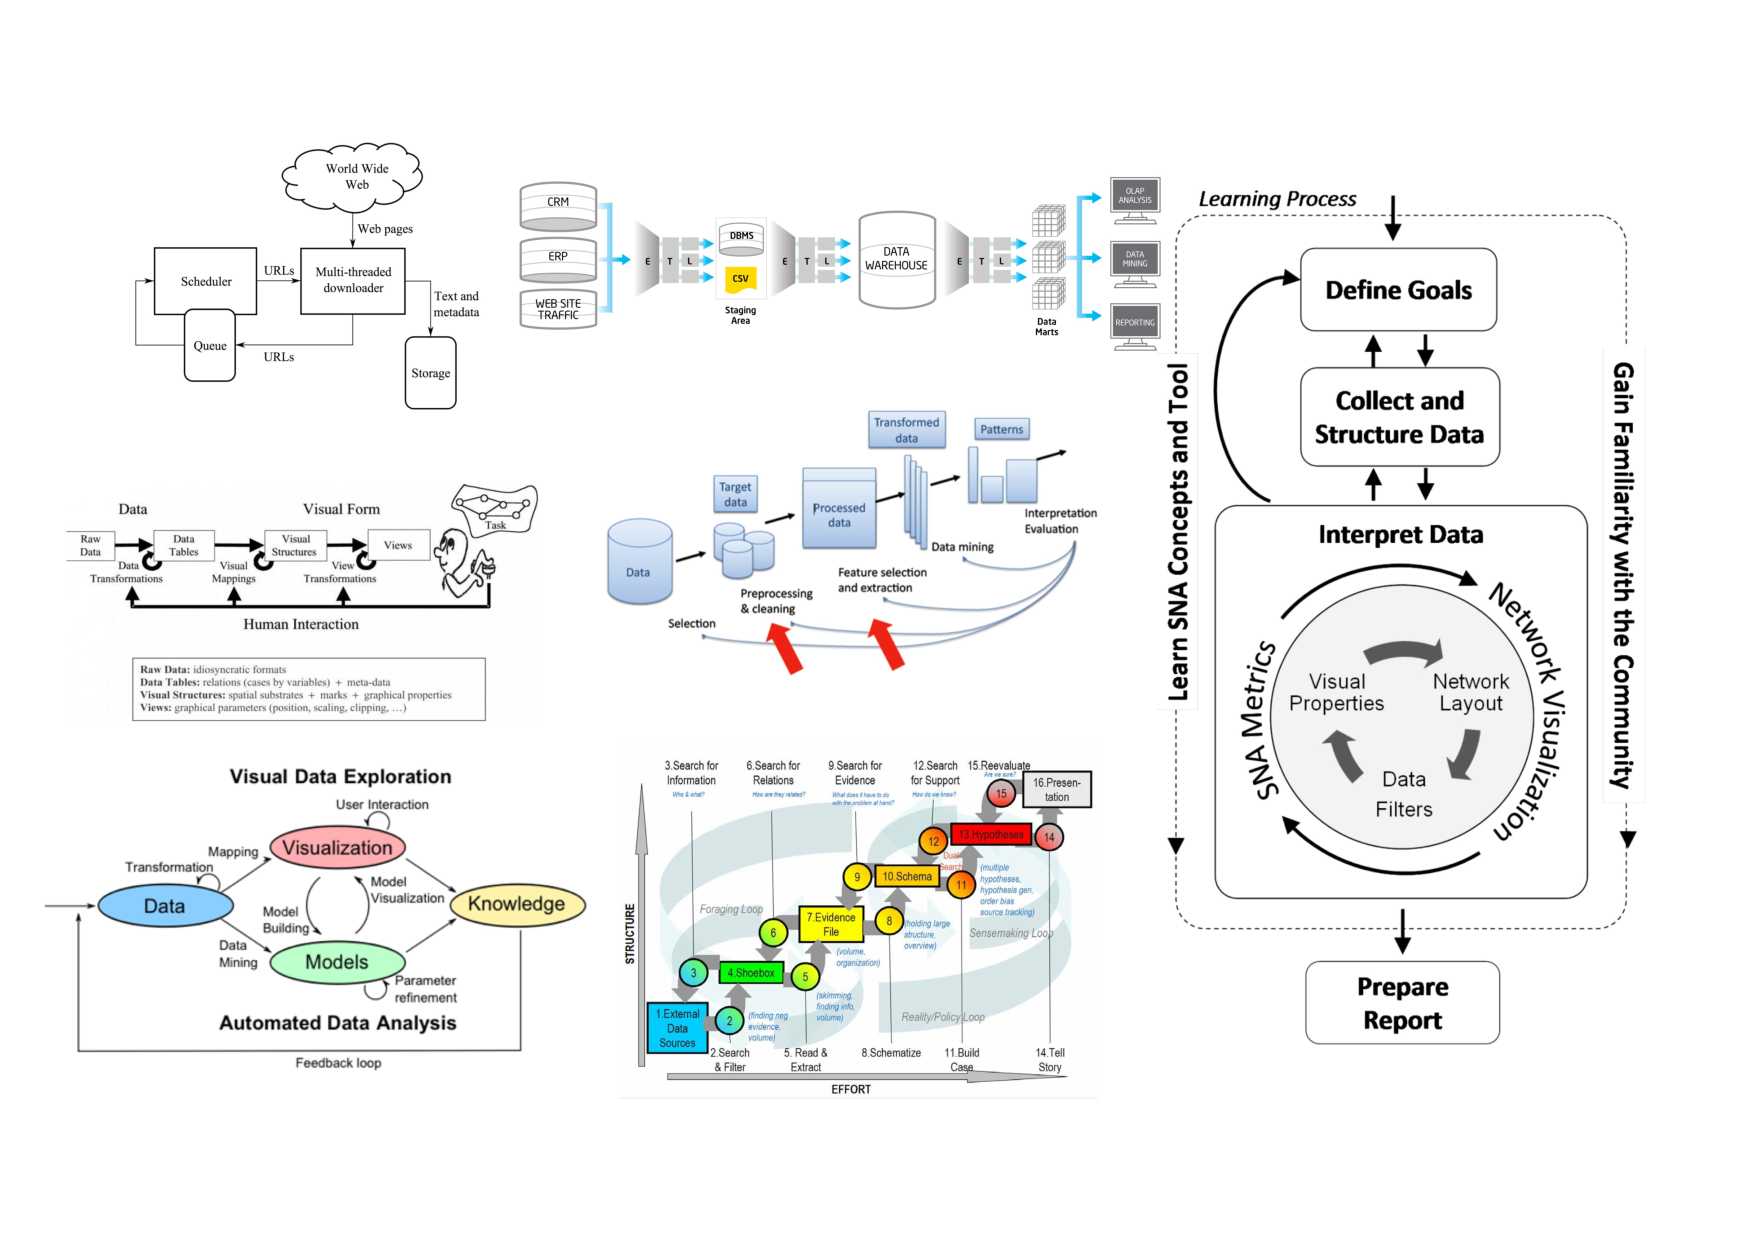
\includegraphics[width=14cm]{figure/Process-models-collage.pdf}
\caption{Process models related to data-driven visual network analytics. The six small diagrams, from top-left: 
web crawling \citep{Wikipedia.org2015}, 
Extract-Transform-Load \citep{Intel2013}, 
information visualization reference model \citep{Card1999ReadingsThink}, 
knowledge extraction from databases \citep{Indarto2013}, 
visual analytics \citep{Keim2010MasteringAnalytics}, 
sensemaking \citep{Pirolli2005TheAnalysis}. 
On the right: Network Analysis and Visualization (NAV) model \citep{Hansen2012DoData}.}
\label{fig:process-model-collage}
\end{figure}

Component-based data-processing pipelines, a technical application of the information visualization reference model, introduce a viable approach for developing reusable pieces of software to support the automation of processes related to social network analysis across application domains \citep{Nykanen2008,Huhtamaki2010Context-DrivenCo-Creation}. To support investigating the social structure among wiki co-creators, for example, \cite{Huhtamaki2010Context-DrivenCo-Creation} present a set of components and a process model for the orchestrated use of the components. A key benefit of the component-based approach \citep{Nykanen2008} is the possibility to integrate existing software tools implemented in different technologies into the data-processing pipeline, given that they can be operated from the command line. The main restriction of the approach is the need to implement the automation through scripting, i.e. writing program code that describes rules for a particular functionality rather than operating a user interface.

The general sensemaking model \citep{Pirolli2005TheAnalysis} divides the sensemaking process into two loops, the foraging loop and the sensemaking loop. To simplify, data is first collected and refined and then transformed into a selection of visualizations and other representations that support sensemaking. The process is iterated as many times as required. Similarly, the process of visual analytics ``typically progresses in an iterative process of view creation, exploration, and refinement'' \citep{Heer2012InteractiveAnalysis}. 

The sensemaking part of the process can be implemented in different ways from purely manual processes where human investigators interact with various user interfaces to conduct the analysis to automated dashboard-centric information systems in which data are collected and processed in runtime. Sensemaking also includes the process of visual analytics \citep{Wong2004VisualAnalytics,Keim2010MasteringAnalytics} that, by default, relies on the availability of software and tools supporting the users. \cite{Heer2012InteractiveAnalysis} give an insightful overview to the specific functionalities that users should be able to operate: 1) specify data and views, 2) manipulate views, and 3) process and provenance their findings.

\cite{Peng2009} builds his definition of reproducible research on three categories: a piece of research is fully reproducible if both the data and code used to are available and, moreover, if the code is executable by anyone. As \cite{Ghosh2013} shows, reproducibility can be approached at many different levels from research policy to detailed technological solutions. Over the last few years, open research practices has become a priority e.g. in Finnish universities\footnote{Open Science and Research at TUT, \url{http://www.tut.fi/en/library/open-science-and-research-data/open-science-at-tut/index.htm}}.

To conclude the review, we note that many of the existing process models are either very general or focus on particular parts of the process. A data-driven visual network analytics approach insists on drawing from a number of process models. For example the use of parallel data sources is often not considered in the process models. Moreover, network analytics introduces specific requirements to the process, importantly including the possibility to calculate node metrics as additional data quantifying the different structural roles of the nodes.

\section{Requirements from the series of investigations}
\label{sec:processmodelrequirements}

Through the series of investigations included in this dissertation, we have shown that visual network analytics is a value-adding approach in exploring and investigating innovation ecosystems and in sharing the findings to others. According to our experience, many of the process-related requirements stemming from the individual investigations are similar. At the same time, many of the investigation-specific analysis processes have insisted us to tailor the process as we have iterated toward the final analysis.

With the data-driven approach, the investigators of innovation ecosystems are able to move fast in the beginning of the process. As the ways of visualizing and investigating a particular phenomenon matures, the investigators may wish continue to follow the phenomena with the support of close to real-time dashboards adding transparency and supporting e.g. longitudinal investigations. The option for automating the process also supports developing these investigative tools toward end-user products for avid innovation ecosystem actors, orchestrators, investigators and policy makers.

The requirements that emerge through the investigations allow us to make way to the third and most important part of results of this dissertation, namely the process model for data-driven visual network analytics. This will answer \ref{objective:processmodel}. This section provides a synthesis of the requirements stemming from the investigations presented in Chapter~\ref{ch:experiments}.

Developed through several rounds of iterations following the Building-Intervention-Evalution cycle \citep{Sein2011ActionResearch}, the core guidelines and requirements for the data-driven visual network analytics process model include the following: enabling manual steps; exploration; transparency; low entry barrier; interoperability; loose coupling; reproducibility; automation;   and continuous data collection. In this dissertation, the requirements presented in this chapter and originally in \ref{pub:ostinato} serve as a design rationale to support the definition of the process model for data-driven visual network analytics, the Ostinato Model. Chapter~\ref{ch:ostinato} describes the model in detail. The next sections introduces each requirement.

% \begingroup
% \captionof{table}{Details on collecting and processing data for the experiments}\label{tab:processreqs}
% \begin{tabular}{p{3cm} p{1cm} p{3cm} p{2cm} p{2cm}}
% \toprule
% Requirement	& Order & Description & Experiment & Origin \\
% \midrule

% Enabling manual steps&1 & & & \\			
% Exploration&2& & & \\
% Transparency&3& & & \\		
% Low entry barrier&4& & & \\		
% Interoperability&5& & & \\	
% Loose coupling&6& & & \\
% Reproducibility&7& & & \\	
% Automation&8& & & \\
% Continuous data collection&9& & & \\

% \bottomrule
% \end{tabular}
% \endgroup

% Table \ref{tab:processreqs} %\href{https://docs.google.com/spreadsheets/d/1o8bqFOYRtAzwMaFiPXr7IrWCoCs77nl7P921AsV3iE8/edit?usp=sharing}{Process model requirements} 
% gives an overview of process model requirements and specifies the experiment in which it was first identified.

\subsection{Enabling manual steps}

While reproducibility is an important long-term objective, at the same time it is key to realize that automating some of the steps may not be feasible when an analysis is conducted the first time or requires intensive tailoring. Therefore, the process should support implementing any of the individual process steps manually. The use of file-based intermediary results is a practical solution in enabling manual analysis steps \citep[cf.][]{Huhtamaki2017ProcessingExperiences}.

\subsection{Exploration}

Visual analytics \citep{Heer2012InteractiveAnalysis} approach is key in enabling users with varied technical skills to collaboratively explore and make sense of a phenomenon. Being able to follow the visual analytics approach, however, requires flexibility from the investigative tools and processes. That is, all the stakeholders of the analysis process should be able to conduct any of the individual steps by themselves even though development of the overall process requires technical development skills.

In the investigations included in this dissertation, we have relied extensively on using Gephi for exploring the networks. At best, however, the whole data processing pipeline from collection to refinement and transformation to visual representation would allow interaction also for non-technical investigators.

\subsection{Transparency}

Developers with extensive technical skills may select to manage the network analysis data throughout the analysis process with a database. Graph databases in particular are appealing for conducting network investigations. To accomplish transparency and flexibility in the process, however, other members of the investigative team will benefit from the option to access the data as files. The use of intermediary results is key in facilitating the transparency and flexibility of the process. Intermediary results refer to data in between the individual steps of the analysis. These data should be available as files in widely used formats, such as CSV and GEXF. In addition to the enhanced transparency, these intermediary results allow for speeding up the analysis process by using cached versions of source data and intermediary results when they have not changed.

\subsection{Low entry barrier}

Analysis of innovation ecosystems and other network-based investigations of complex phenomena require extensive domain knowledge, and hence insist on active participation from domain experts (often without extensive technical expertise) throughout the analysis process. This requirement further underlines the need for transparency of the individual steps of the analysis process.

\subsection{Interoperability} 

Despite the clear benefits of an integrated all-in-one tool for data-driven visual network analytics \citep[cf.][]{Freeman2000VisualizingNetworks}, there will always exist individual tools that offer features not included in the all-in-one tool. Therefore, the investigative team should be able to use a number of existing analytics tools with high usability and rich interactivity including Gephi, NodeXL, KNIME and Tableau for conducting the individual parts of the analysis. Moreover, provisioning the visualized networks and other outputs of the analysis should be possible through dashboard built with Web technologies such as D3.js, DC.js, GEXF.js and the likes. 

\subsection{Loose coupling} 

At best, data-processing pipelines can be built with a range of tools and components implemented in different technologies. Loose coupling is key in enabling this kind of flexibility that allows the introduction and use of new expressive tools from individual software components to full-featured applications as they become available to the investigative team. Many of the tools introduce new opportunities for advancing the analysis process but generally it is not possible to integrate these tools to a data-processing framework in program code, i.e. in native application programming interface level.

Data collection and pre-processing routines in the investigations described in Chapters~\ref{ch:experiments} and \ref{ch:ecosystemnetworks} are implemented in Python using a collection of software modules for additional expressiveness. In addition, we use OpenRefine for cleaning data and Gephi for laying out the networks and calculating some of the network metrics. In addition, we use NetworkX to calculate network metrics in Python for automation. For larger networks, we point to Snap.py\footnote{Snap.py - SNAP for Python, \url{http://snap.stanford.edu/snappy/}}. Being able to use third-party routines for calculating different state-of-the-art network metrics presents an example of extendability that an investigative team will benefit. Tableau allows for visual analytics with a user interface and therefore serves as an example of a tool that many of the investigative teams will use due to loose coupling. 

\subsection{Reproducibility}

In the data-driven visual network analytics approach, reproducibility is first and foremost a technical quality of the process: the investigative team should be able to repeat an investigation or one or more parts of the analysis process and reproduce the results. Reasons for the need to rerun the process include, among others, updates on the source data, development steps of the analysis process, and the introduction of completely new processing steps as well as new tools that insist on the use of a particular data format or extending the existing data. Moreover, dynamic sensemaking for complex phenomena mandates being able to refresh the data and derive new results with updated data. Reproducibility at this technical level also allows the investigative team to release the process, data and results to other researchers interested in the phenomena under investigation.

\subsection{Automation}

Being able to develop automatically updating dashboards as needed gives the investigative team the opportunity to continue observing a particular phenomena of interest over time. It is expected that production-ready analysis processes for dashboards will operate without supervision; however, in the context of exploratory research, some requirements may be relaxed. 

Automation is a key requirement should one decide to implement a dashboard for an up-to-date view into the structure of Demola, EIT Digital, Tekes Young Innovative Companies program or the Finnish innovation ecosystem.

\subsection{Continuous data collection}

Persistent processes for collecting data are often needed, particularly when the investigators wish to tap into social media to capture both the structure and structural dynamics of a phenomenon. Twitter, for example, currently provides only limited access to its historical data, and even then data on followers and friend connections between users do not include timestamps. At times, collecting the data takes days or weeks or ``forever'' to complete, due to throttling or other technical limitation or the sheer size or the dynamic nature of source data.

While the collection process of the Innovation Ecosystems Network Dataset \citep{Rubens2010LeveragingMoves} falls outside of the scope of this dissertation, we want to point that out as an example of a data-collection process that has to run continuously in order to keep the views into innovation ecosystems up to date. 

\chapter{Ostinato Model for data-driven visual network analytics}
\label{ch:ostinato}

In this chapter, we describe Ostinato Model, a process model for data-driven visual network analytics of innovation ecosystems. Ostinato Model answers \ref{objective:processmodel} and represents the main contribution of this dissertation. The Ostinato Model is developed over the series of experiments presented in Chapter~\ref{ch:experiments}. Requirements identified through the investigations and existing process models Chapter~\ref{ch:processmodels} are the key drivers in developing the Ostinato Model.  The Ostinato Model was first presented in \ref{pub:ostinato} in the context of social media studies. Here, we discuss the Ostinato model in particular in the context of investigating innovation ecosystems. This chapter is a revised version of a section in \ref{pub:ostinato}.

In music, the word \emph{ostinato} refers to both a repeating musical pattern as well as a composition that contains a repeating musical pattern. Like the repeated rhythms and melodies in Ravel's Bolero in Figure~\ref{fig:bolero-ostinato} or distinctive in post-rock\footnote{Categorizing music is  debatable at best. However, music that falls under the post-rock category has been playing in the earphones of the author of this dissertation for hours and hours while conducting the investigations and writing this manuscript. For a sample, please refer to \href{https://www.youtube.com/watch?v=fD2HgZMdxOI}{Magyar Posse}.}--small innovations are explored with each iteration, and some are incorporated into the melodic narrative--we apply the musical concept of ostinato to a cycle of user-centric exploration and automation that builds transparency of authorship for evidence-based decision making.

\begin{figure}[htb]
\centering
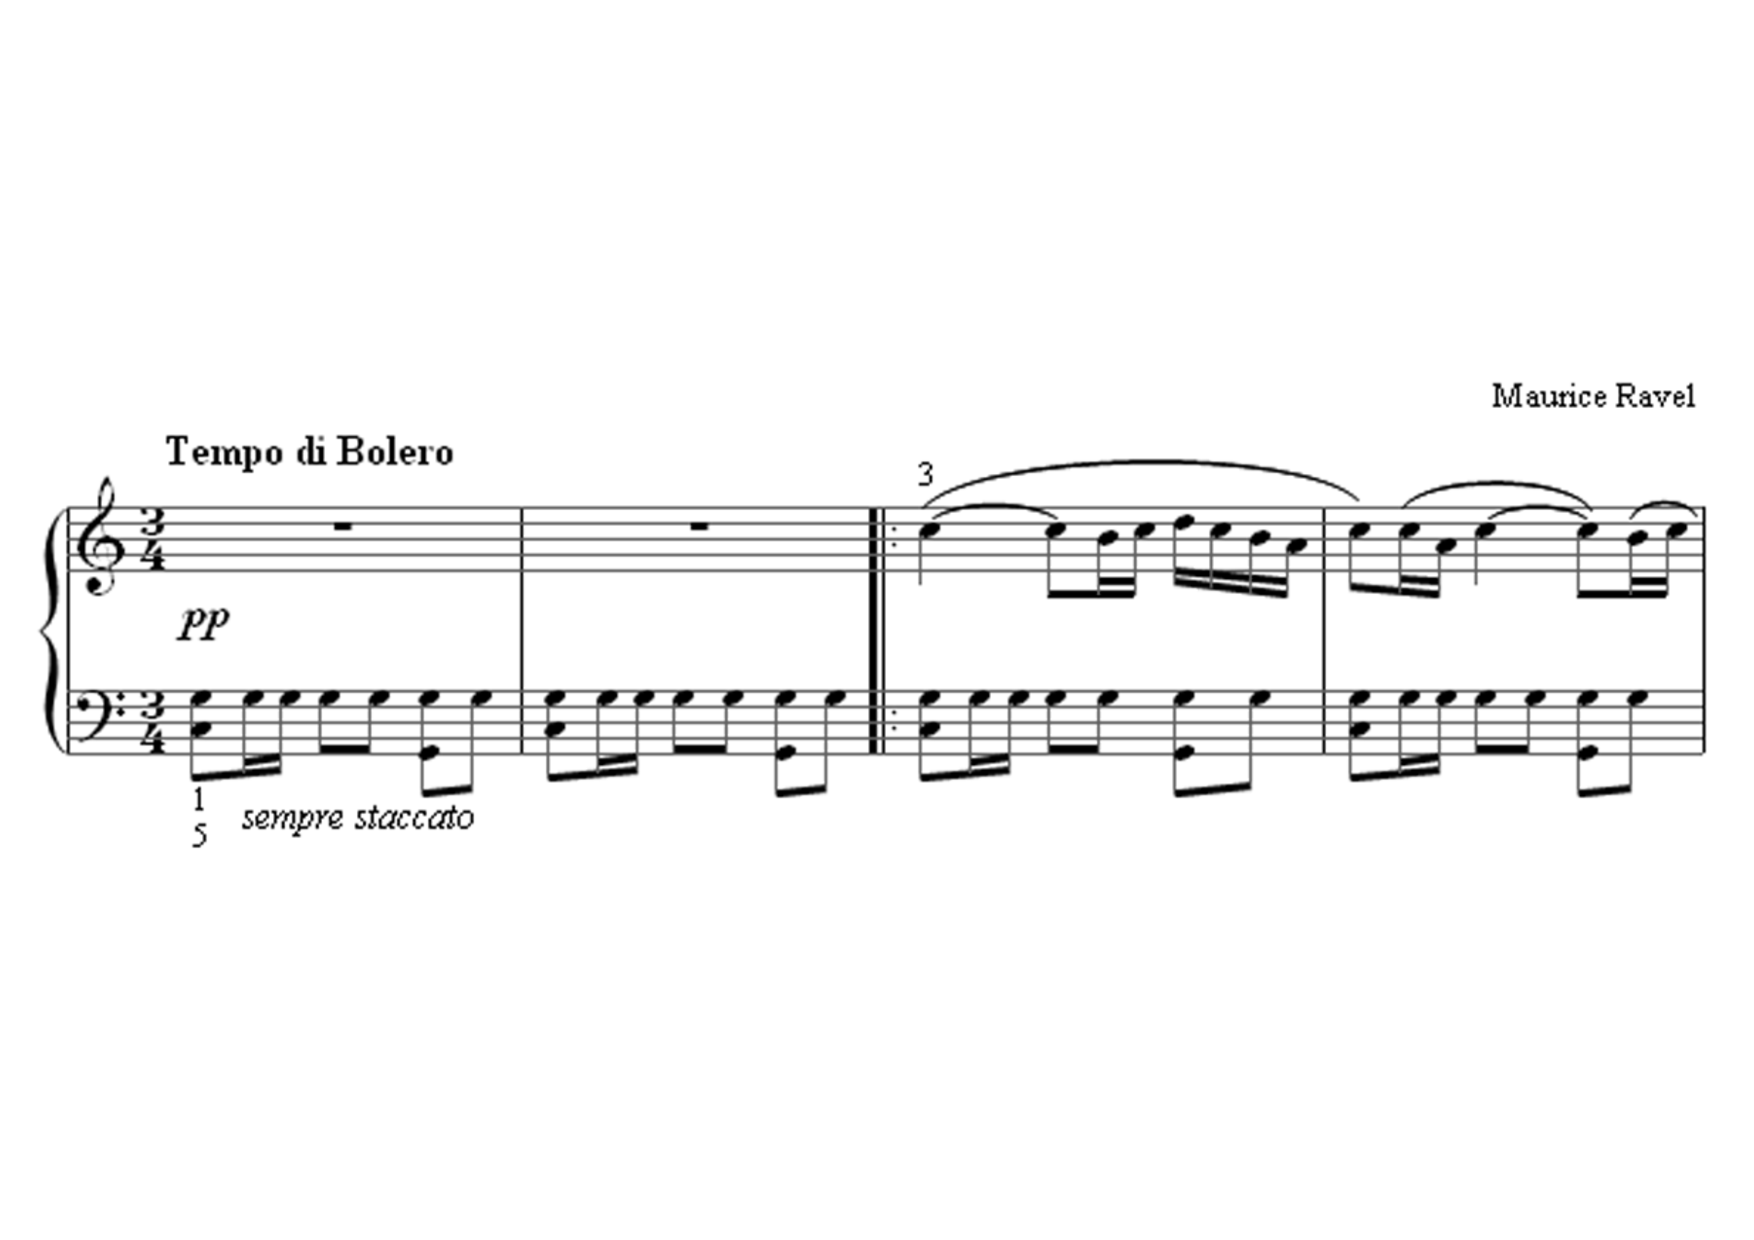
\includegraphics[width=12cm]{figure/Bolero.pdf}
\caption{Ostinato patterns from Bolero's Ravel \citep{Mawer2000TheRavel}}
\label{fig:bolero-ostinato}
\end{figure}

In the Ostinato Model, the phenomena under investigation are modeled as a network, and interactive visualization tools are used to conduct the investigative process. Imperatively, interaction is extended to all the different phases of the analysis process through transparency and the definition of explicit phases. Network analysis introduces a relationship approach to investigating the structure of many kinds of phenomena. Network analysis allows for the exploratory analysis of the social roles of network actors and the complexity of relationships, as well as for quantifying the structural properties of the network representation of the innovation ecosystem under investigation.

A key aspect of the Ostinato Model is the focal point of the user--here, the investigator of an innovation ecosystem--in the investigative process. Putting the investigator to the center of the process answers to the call for data scientists \citep{Davenport2014BigOpportunities}, the almost mythical multi-skilled individuals that are capable of individually running the whole investigative process from collecting data to analysis to deep sensemaking in the domain of interest, by allowing both experts of the domain under investigation, developers of the technical process as well as e.g. quantitative analysis specialists to have equal means to take a proactive role in the investigative process. Moreover, the Ostinato Model defines an overall structure for the data-driven investigative process that supports the coordination between the individual phases of the process and therefore allows all the members of the investigative team to contribute to the implementation of different phases of analysis and, importantly, to the sensemaking on structures and mechanisms emergent in empirical data representing an innovation ecosystem.

The Ostinato Model is developed over a series of experiments in investigating innovation ecosystems with an action design research approach. It is built on existing process models and previous work presented in Figure~\ref{fig:process-model-collage} and it takes into account the process requirements presented in Chapter~\ref{ch:processmodels}. Figure~\ref{fig:ostinato} shows a diagram of the Ostinato Model. Each step is described in the following sections.

\begin{figure}[htb]
\centering
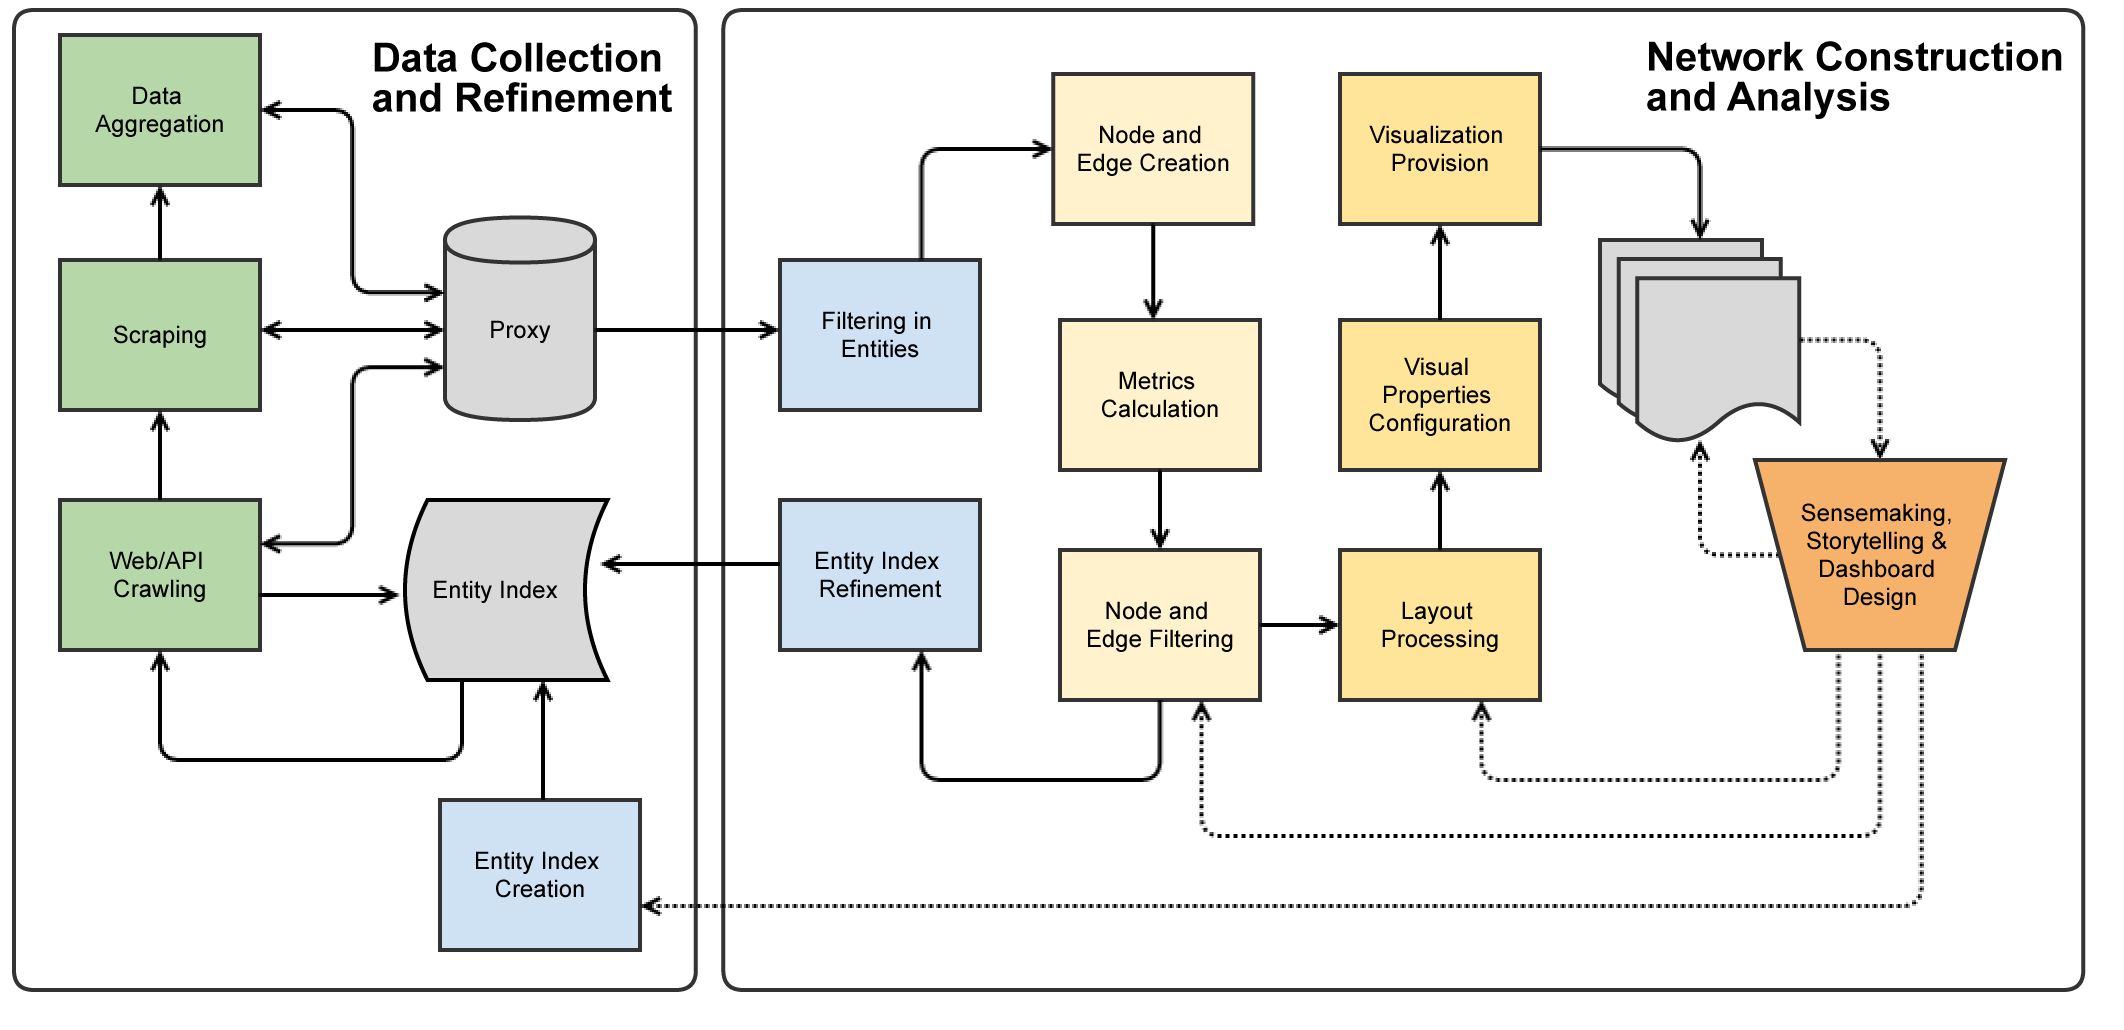
\includegraphics[width=1.0\textwidth]{diagram/kredible_net_process_model-v07.png}
\caption{Ostinato Model--user-centric data-driven process model for visual network analytics}
\label{fig:ostinato}
\end{figure}

Phase 1: Data collection and refinement

\begin{enumerate}
\item Entity index creation
\item Web/API crawling
\item Scraping
\item Data aggregation
\end{enumerate}

Phase 2: Network construction and visualization

\begin{enumerate}
\item Filtering in entities 
\item Node and edge creation
\item Metrics calculation
\item Node and edge filtering
\item Entity index refinement
\item Layout processing
\item Visual properties configuration
\item Visualization provision
\item Sensemaking, storytelling \& dashboard design
\end{enumerate}

\section{Phase 1: Data Collection and Refinement}
\label{subsec:modelphase1}

The general rules of data-driven analytics apply when operating with the Ostinato Model: collecting and cleaning the data will, in most investigations, consume most of the time and resources available for the investigation.

\subsection{Entity index creation}

In some investigations, the source data can be collected in full whereas in others only data on entities that are relevant for the analysis need to be collected. The entities for which data is collected are defined by boundary specification. In investigating the connections between companies taking part in Young Innovative Companies program in \ref{pub:tekesyic}, the list of companies defines the starting point of the analysis \citep{Huhtamaki2012NetworksFinland}. In studying the structure emerging from individual deals and alliances around Google and Motorola Mobility, boundaries are set at two steps from the focal companies \citep{Basole2012UnderstandingApproach}.

\subsection{Web/API crawling}

Collecting the data is the most heterogeneous step in the data-driven visual analytics process \citep[cf.][]{Salonen2013ChallengesMedia}. Possible source data potentially includes everything digital, from proprietary offline documents and document collections to spreadsheets to Web APIs (application programming interfaces) to Web sites that are designed primarily for human interaction. 

Similarly, the functionality required to collect the source data can range from relatively simple reading of individual documents to functions similar to a fully featured Web crawler. Compared to crawling random websites, Web APIs are, by default, more straightforward for data collection as they are often designed to support reuse \citep{Vinoski2008}. At best, source data is available as linked data \citep{Bizer2009}, i.e. data that has a clear structure with individual facts that can be interconnected with the help of unique identifiers to enable referential integrity. 

Thomson Reuters SDC provides a functionality for extracting data on alliances on basis of different search criteria, therefore crawling is not required. Crawling is, however, utilized extensively in collecting the IEN Dataset \citep[see][]{Rubens2010LeveragingMoves}. Moreover, in \ref{pub:tekesyic} we use Twitter REST API for crawling the follower data on companies in Tekes YIC program.

At the end of the crawling phase, a set of web resources, or rather their representations in Hypertext Markup Language (HTML) or some other format, is made available in a local database or other storage, a proxy that significantly speeds up the subsequent processing steps.

\subsection{Scraping} 

Once the raw source data is available locally, the next step is to filter, select and distill the utility data relevant to the analysis process. Scraping refers to the process of distilling data from documents that are published to the Web first and foremost for humans to use. This kind of data extraction and cleaning is sometimes referred to as data wrangling \citep{Kandel2011}. Scraping can further be seen as a form of the Extract, Transform, Load (ETL) process that is often applied in the context of data warehousing or other business intelligence processes to collect data from different sources to be refined and normalized and finally loaded into a consistent database for later use \citep{Petschulat2010,Vassiliadis2009}. 

Scraping-like functionality is required to distill the data from the spreadsheets in Excel format exported from Thomson Reuters SDC. We use JSON to represent the data representing individual deals and alliances. To support non-technical investigators access to the data, the use of CSV should be considered for representing intermediary results for added transparency and lowered entry barrier.

Using Wikipedia data in analyzing the structure of an innovation ecosystem is an example of scraping. When collecting data from Wikipedia on Finnish Young Innovative Companies, for example, the investigators are particularly interested in the facts presented in the Infobox section of the page \citep[cf.][]{Huhtamaki2007CommunityEcosystem}. To collect this data, one can take advantage of the HTML markup on the page to specify the semantics (meaning) of the different pieces of text. Each of the facts is represented as a table row including two cells, the first of which includes the label specifying the type of the fact and the second includes the actual value. Moreover, the value is also represented as a link to a separate page. These pages have to be included in the entity index for crawling and scraping additional facts relevant to the investigation.

\subsection{Data aggregation}

In contrast to data-driven social media studies in which data originates from an individual social media service, the complex context of innovation ecosystem investigations often insists on using several sets of data in parallel. This implies that in most investigations, linked data is not readily available and, therefore, links between individual sets of data have to be constructed through the creation of unique entity identifiers that allow referential integrity. 

In innovation ecosystem investigations, the name of the company or another actor is sometimes the key data point that can be used to identify an entity. In \ref{pub:multiscopicfinland}, we use actor names to find entities that appear in more than one dataset. To take into account differences in the spelling of the names, we apply OpenRefine\footnote{OpenRefine is an open source tool for working with messy data, \url{http://openrefine.org/}} to harmonize the names through a semi-manual process. In studying whether co-author networks show small-world properties, \cite{Newman2001TheNetworks} uses author names with and without additional initials to create upper and lower bounds for network measurements. String matching \citep{Navarro2001AMatching} and named entity recognition \citep{Finkel2005IncorporatingSampling} are examples of machine learning-based methods to support automation for creating unique identifiers for actors. 

\section{Phase 2: Network construction and analysis}
\label{subsec:modelphase2}

Once the data is available in a local proxy, the utility data has been extracted from the source documents, and data from different sources has been aggregated into a consistent set of linked data, the construction of the network representation of the innovation ecosystem under investigation can begin.

\subsection{Filtering in entities}

The network construction phase starts with a selection of the entities to be included in the network. The selection of nodes is guided by the boundary specification designed and defined by the investigative team. At least two approaches exist to implement the selection: starting from a list of entities and rule-based entity inclusion.

To continue the Finnish YIC example in \ref{pub:tekesyic}, we start from the list of companies participating in the program and continue to include all the individuals and investors directly connected with the company. Moreover, we include companies that are connected to the companies already in the sample through an investment or acquisition. For investigations on the Finnish innovation ecosystem and EIT ICT Labs in \ref{pub:multiscopicfinland} and \ref{pub:eitictlabs}, respectively, companies are selected on basis of their location. In both investigations, directly connected companies, individuals and investors are included in the sample.

A key reason to separate the selection of entities from node and edge construction is to support the transparency, reproducibility and extensibility of the process. To create a shared understanding of the results of the analysis, it is absolutely vital that all the investigators taking part in a particular network investigation are able to access and understand the original raw data, in addition to any constructed variables, and the various analytics and metrics that represent the network; this means that investigation participants need access to data from raw to refined. According to our experience, answering specific questions raised by anyone interested in an investigation, drawing conclusions, generalizing the results, developing more specific and potentially more interesting questions all depend on transparency of the data available and used for the analysis.

\subsection{Node and edge creation}

Creation of the network is of course a core part of the data-driven network analysis process. Network creation boils down to the creation of nodes representing the actors and the creation of edges representing the connections between the actors. Several options are, however, available when specifying details of the network creation process. First, the network can be either one-mode or two-mode. In one-mode networks all the nodes are of same type: startup companies or investors, for example. Connections between the nodes are formed through relationships: investments, affiliations to individuals, acquisitions and transactions. In two-mode networks, there are two types of nodes, for example, startup companies and individuals related to them. Hypergraphs and bipartite graphs are examples of means to visualize two-mode networks \citep{Jesus2009,Freeman2009MethodsVisualization}.

Further, the connections between network nodes can be either weighted or dichotomous. The strength of a connection can be expressed with weighted connections. In either case, the connections may be undirected or directed. Moreover, temporal dimension can be included in networks if the data used to create the connections is time-stamped. As we show in \ref{pub:demola} and \ref{pub:mobileecosystem}, with temporal data, insights about the evolution of the network can be provided.

In all of the investigations included in this dissertation, we have eventually decided to use multimodal networks for representing the innovation ecosystems under investigation. We assume that the main reason for this is the exploratory, descriptive nature of the investigations that highlights the importance of the system-level view over detailed measurement of structural properties. 

\subsection{Metrics calculation}

Network metrics enable quantifying a variety of structural properties, both in network and node level. These range from simple metrics such as node degree (indegree, outdegree) \citep{Freeman1978CentralityClarification} and betweenness to PageRank \citep{Page1999TheWeb} hub and authority values with HITS \citep{Kleinberg1999AuthoritativeEnvironment} and other more sophisticated measures. Whereas in principle, every metric can be calculated for all of the networks and their nodes, in practice this is not always feasible due to reasons of efficiency. Moreover, new metrics for networks are being developed continually, and the investigative team is likely to find--or develop--new metrics that fulfill specific investigative purposes. From an implementation viewpoint, it is unlikely to find one tool that supports all the metrics the team wishes to use. Therefore, a combination of tools may be required to calculate the metrics. Loose coupling allows this.

As part of metrics calculation, network metrics for the network representation should be stored for later usage. For transparency, a list of exported network nodes and edges should include the various metrics used. In practice, node and network metrics must be recalculated after each change in the network structure; however, reference to previous calculations is often needed e.g. for analyzing the change in the structural position of nodes.

The selected network structure dictates the metrics that can be calculated for the network and individual nodes. A one-mode network that has directed and weighted edges allows using the widest range of node and network metrics. In a multimodal network of companies, investors, and individuals, for example, metrics such as density or authority may not be fully relevant as e.g. investors can never be connected to other investors if the connections are based on investments.

\subsection{Nodes and edge filtering}

A key limitation of visual network analysis is the amount of space available, both on screen and particularly on paper, to present the visualization. Depending on the level of detail required in the analysis, hundreds or thousands of nodes can be presented in one visualization view. For networks of tens of thousands of nodes and more, only more general structures and patterns can be observed from a visualization. 

Two means exist to address this limitation: the best option is to allow the visualization users to filter in and out nodes and edges. If the end-user tools used to present the visualizations do not allow filtering, it can be done as one part of the automated process. Often, reducing the size of the visualized network is accomplished with a combination of filtering out edges that have the least amount of weight as well as filtering out nodes that: 1) are left without edges; 2) have a value of the degree or some other a network analysis metric under a specified threshold; or 3) are (not) of particular type (even though this can already be taken into account when filtering in the entities used to construct the network in the first place).

\begin{figure}[htb]
\centering
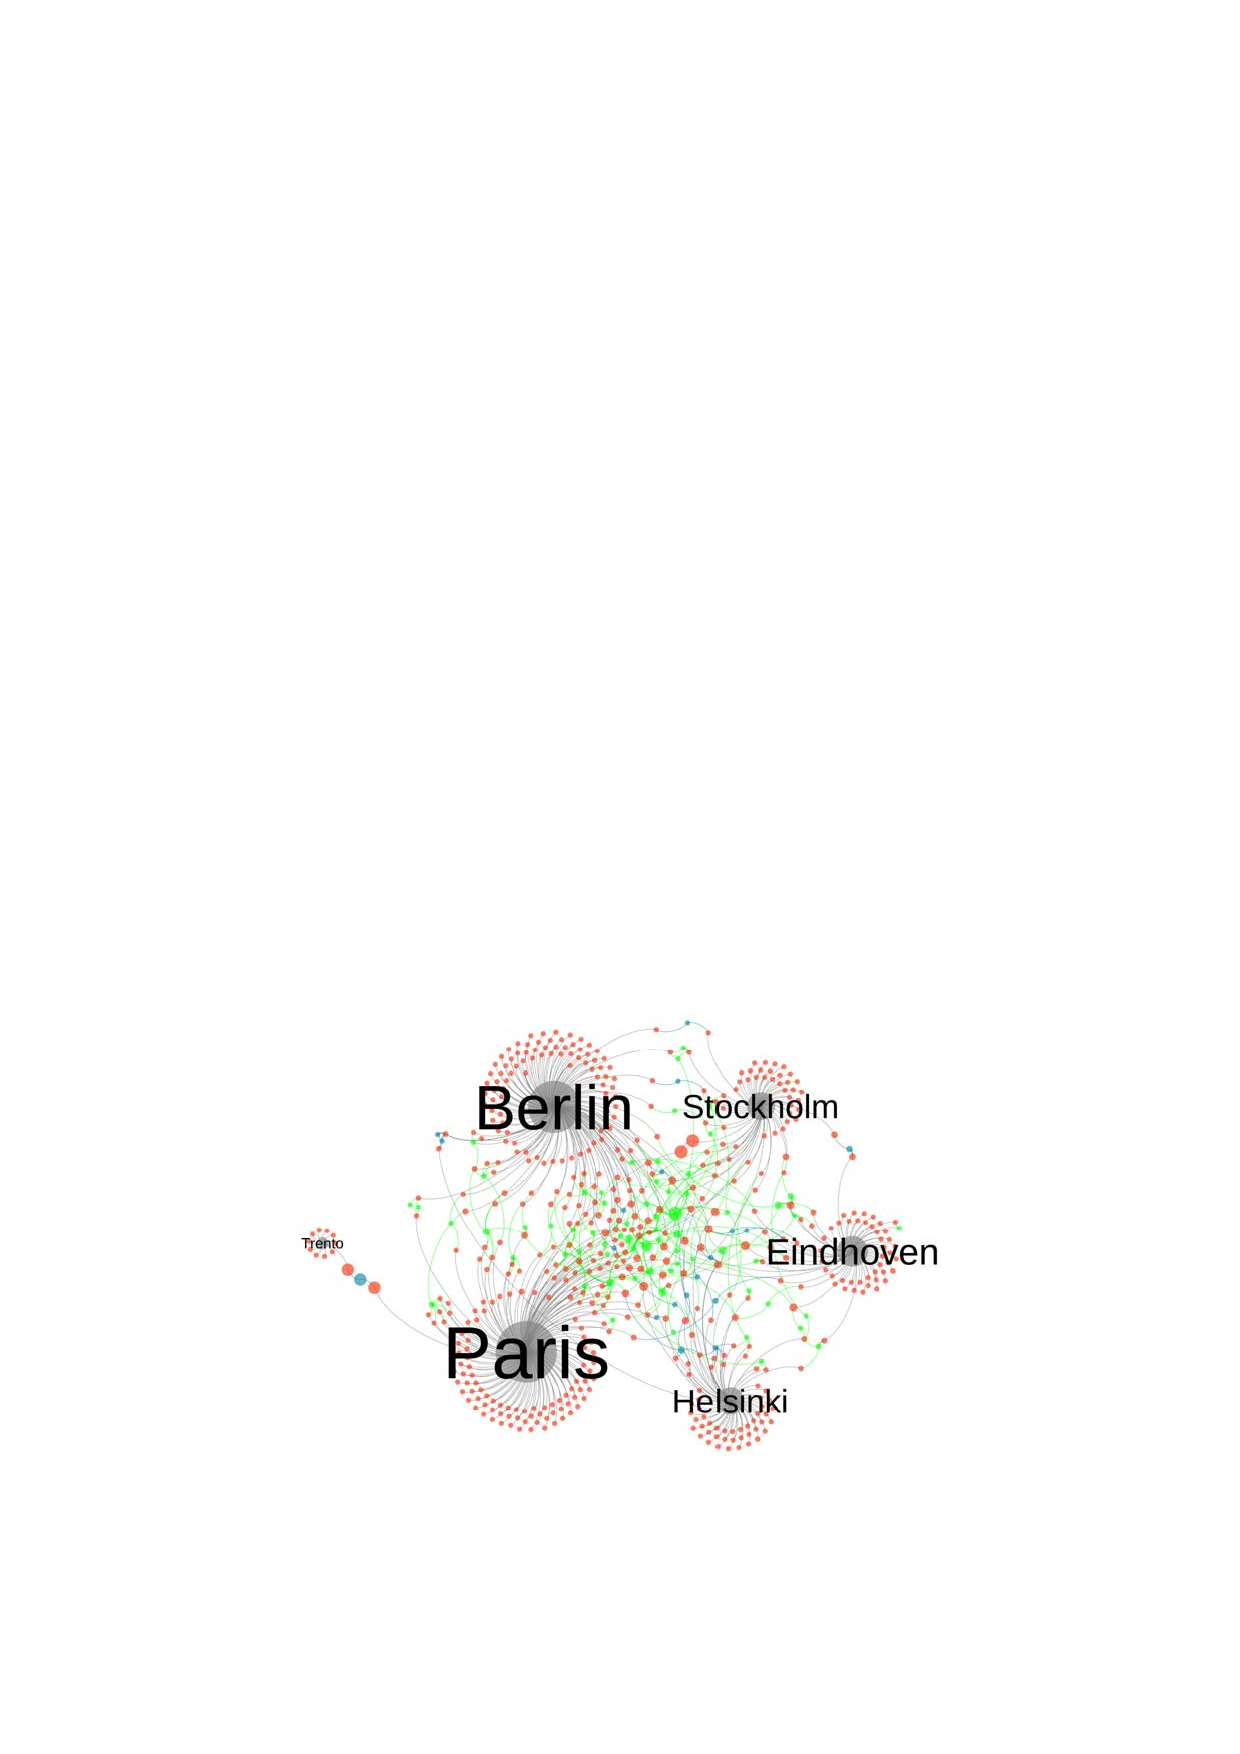
\includegraphics[width=12cm]{figure/eitictlabs-top10percent.pdf}
\caption{Top 10\% of individual, companies and investors connecting EIT ICT labs co-location cities according to their betweenness. The role of venture capital investors as enablers for mobility becomes evident.}
\label{fig:eitictlabs-top10percent}
\end{figure}

In Figure \ref{fig:eitictlabs-top10percent} in \ref{pub:eitictlabs}, we provide a filtered version of the network structure of EIT ICT Labs to highlight the importance of venture capital investors in connecting the different co-locations centers and therefore in enabling mobility in Europe. The nodes are filtered in according to their betweenness centrality. In \cite{Jarvi2016DismantlingLinkages}, we apply filtering to investigate innovation ecosystem by dismantling ``the network structure through a procedure that resembles peeling an onion.'' 

\subsection{Entity index refinement}

At this stage of the process, the network representation of an innovation ecosystem under investigation is constructed and the required metrics are calculated for each of the nodes. Depending on the boundary specification applied in the investigation, the network is either ready to be visualized or, alternatively, additional data can be collected to complement the network. Revisiting the Finnish Young Innovative Companies case in \ref{pub:tekesyic}, the boundary specification is designed to include all the individuals involved in one or more of the companies in YIC program as well as all the other companies the individuals are or have been affiliated with. Moreover, the data includes all the investors that have invested into any of the companies as well as all the companies that have acquired any of the YIC companies.

Entity index refinement has a particularly important role when using multiple sources of data. If, for example, boundaries of the innovation ecosystem under investigation are set to two steps from the focal companies, the actors coming in through the first step should be taken into account across datasets.

\subsection{Layout processing}

The principle of processing network layout is simple. Nodes are given a position in two-dimensional space in a way that network structure is revealed in an expressive, intuitive way. Despite the simplicity, novel layout algorithms have been developed over several decades.

In the investigations included in the dissertation, various stakeholders found a specific implementation of force driven layout, Force Atlas, to be particularly suitable for laying out networks representing innovation ecosystems at different levels. In fact, Force Atlas is used in all the investigations included in this dissertation. Force Atlas is implemented in Gephi \citep{Bastian2009Gephi:Networks} and can be used as a batch process with the help of Gephi Toolkit\footnote{Gephi Toolkit, \url{http://gephi.github.io/toolkit/}}. 

In practice, the parameters of the layout algorithm must be adjusted manually for a particular kind of a network before fully automating layout processing. Alternatively, the layout can be processed with the user interface version of Gephi and the resulting network, including the X and Y coordinates for each node, can be exported as part of the network representation in GEXF or other suitable format.

Storing the network layout data is particularly important for improving the efficiency of the analysis process, as well as for reducing investigators’ cognitive load and for promoting transparency. In particular, it is important that after the data is refreshed, the investigators are able to find the pre-existing nodes in an area of the network where the nodes were previously located. This stability can be achieved by inserting the existing positions into the network data before re-running the force driven layout algorithm. In most cases, investigators will find the pre-existing nodes close to the initial area of the network.

Future work is needed to determine how features such as layout algorithms, e.g., those implemented into NodeXL, could be used as a component of data-driven visual network analysis pipelines. 

\subsection{Visual properties configuration}

There is a limited set of possibilities for defining the visual appearance of a network. Nodes have size, color and perhaps a border and shape as elected visual features. Edges have color and width.

Both node and edge properties originating from the source data as well as node metrics can be used to define the visual properties of nodes and edges. In our investigations, node size in most cases represents its betweenness centrality and node color the type of the actor it represents. At best, visual properties are defined as part of the automated pre-processing routines instead of selected manually e.g. in Gephi.

Allowing the user of the visualization to select and change the visual properties according to node metrics and other node properties is perhaps the easiest way to allow end user interactivity in network analysis. Depending on the tools used by the investigators to conduct the analysis, the visual properties of nodes and edges can continue to be tweaked as part of the interactive analysis process.

\subsection{Visualization provision}

At this stage, a network has all the required information available and therefore can be visualized. The means to finalize this step depend greatly on the tools that have been selected for use by the investigative team. In most cases, however, the created network is serialized into a file following a selected vocabulary or format for representing a network. These vocabularies and formats range from different CSV based applications to XML-based languages designed for representing networks.

A minimum approach to provision the network visualizations is to export network data in GEXF or other suitable format and place the resulting file into a folder from where a library such as Gexf.js can access it. More generally, viewer composition scenarios can include the following:

\emph{Scenario 1}. Network viewer component with fixed functionality, i.e. following a fully descriptive approach. Visual properties such as node size and color need to be defined into the data during its processing. Gexf.js is an example of such a component that we have found useful in adding value to a fully static PDF-based approach in disseminating network visualizations.

\emph{Scenario 2}. Implementing a dashboard with Web technologies, more specifically frameworks such as Highcharts, D3.js, Crossfilter.js, DC.js and others. In this case, tailored interactive features for data exploration can be provided to the user, adding options for representing network data. 

\emph{Scenario 3}. Using full-feature explorative analytics tools such as Gephi, NodeXL and Tableau, which can be used to further process the data and to connect source data to visual properties of the visualization. The key here is to produce visualizations rich-enough in data that the analyst can fully utilize the critical properties of the chosen analytics tool for investigation and exploration. In Gephi, for example, it is useful to include attribute data for nodes to assist network filtering in a way the investigator desires to do.

\subsection{Sensemaking, storytelling and dashboard design}

While information visualization includes data transformation, representation, and interaction, it is ultimately about harnessing human visual perception capabilities to help identify trends, patterns, and outliers. Sensemaking has its roots in cognitive psychology and many different models have been developed. Sensemaking procedures are cyclic and interactive, involving both discovery and creation \citep{North2006}. During the data collection and refinement phase, an investigator searches for representations. In the network generation phase these representations are instantiated, and based on these insights the representation may be shifted, to begin the process again. Sensemaking is closely linked to the insight objectives \citep{Konno2014}, and the Ostinato cycle of exploration–automation is key in achieving actionable insights that innovation ecosystem investigators, analysts, and orchestrators can utilize.

When sensemaking requirements are satisfied for investigators and other users, steps of the Ostinato process can be formalized with automated procedures for iteration over time. Key actors, relationships and events of the network can be incorporated into dashboards that will track changes in critical assumptions and into stories that will share vision for actionable change.

\section{Utility and added value of the Ostinato Model}

In this dissertation, Ostinato Model, a new process of data-driven visual network analytics is developed and described. The Ostinato Model contributes to the call for more expressive means for supporting innovation ecosystem investigations in two ways. First, it can be applied to support the data-driven investigations of innovation ecosystem structure and dynamics. Second, for validity and reliability of these investigations, it is key to increase the transparency of the processes behind the data originating from various digital sources.

Moreover, the Ostinato Model contributes to the data-driven network investigations of innovation ecosystems in three different ways. First, the network approach has great strength in supporting the exploratory investigations of the patterns in between actors of innovation ecosystems. Second, referring specifically to the first phase of the Ostinato Model, data-driven approach allows tracking down processes over the boundaries of individual sources of innovation ecosystem data. Third, user-centricity of the data-driven process adds to the transparency of the process itself, therefore providing means to triangulate different phases of data refinement and transformation and allowing different stakeholders of investigations to take as proactive role as they wish in moving forward a particular investigative process.

Due to the continued and rising interest in big data analysis, new tools are continually introduced to support investigative work. Despite the development of all-in-one tools, a combination of tools is likely to continue to provide more flexibility in accessing and aggregating data and in processing and analyzing it. Finding a balance between user interface-operated low barrier tools and expressive computational strategies that require technical knowledge is key in making the investigative process as productive as possible while maintaining transparency and process flexibility.

The proposed Ostinato Model for user-centric, process-automated, data-driven visual network analytics meets many of the requirements outlined in \ref{sec:processmodelrequirements} for the exploration–automation cycle recommended for developing shared understanding.

Using files rather than databases for representing intermediary results supports both loose coupling and transparency of the process. It also allows for implementing some of the steps manually, if seen feasible, and the flexibility of the process in general is increased.

Allowing exploration boils down to the selection of the end user tools for investigators to visualize and explore the data. If a rather static tool such as Gexf.js, for example, is used, the user is limited to browsing and searching the data. If importing the data into an exploration platform such as Gephi or NodeXL is permitted, it is possible to provide the user with rich node and edge data, enabling them to continue their explorations with more independence. The availability of expressive visual analytics tools, such as Tableau, adds to investigation options of analyzing network data, either as a network or using node and edge level data to provide new inspirations for other kinds of data analyses.

Low entry barrier is enabled through making intermediary results available to all the members of the investigative team. As the process is repeatable and its individual steps are automated, new projections of the data can be implemented in an iterative and incremental manner. Implementing completely new steps of analysis becomes possible even without technical skills. Automating the steps, however, requires developers’ attention. The Ostinato Model requires a multidisciplinary data science team or the somewhat mystical multi-skilled data scientist \citep[cf.][]{Davenport2014BigOpportunities} to conduct the investigation.

Interoperability can be built into the computational approach. This requires that the technical architecture is flexible enough to permit different software components and tools--that may be implemented with different technologies--to be introduced into the process. When an analysis pipeline is built completely from scratch, it is recognizably important to minimize the number of technologies used. However, moving fast and in an agile manner is an objective we claim can be achieved when existing tools can be integrated into the pipeline to implement the individual steps of the analysis process and to provide the visualizations to investigators and other end users.

Reproducibility is both a technical and a policy requirement. For an investigative team revisiting or extending an existing investigation, the availability of runnable code, source data, and intermediary results provides a fruitful starting point. Moreover, the results of reproducible studies can be published in a way that both data and runnable code are available, providing a solid foundation for others to add their contributions as well. A reasonable proposition is that such a piece of knowledge draws attention from other researches and therefore has increased potential for impact. Automation is a key requirement in reproducibility, as well as in creating dashboards that continues to update visualizations of the phenomenon under investigation, sometimes in close to real time.  

Setting up persistent data-collecting routines requires, in general, a programmatic implementation and must be designed and implemented case by case. To maintain the transparency of the process, it is important that the investigators are able to access both the raw data as well as to track down the individual steps used to derive the data that is eventually used for the analysis and visualizations.

More generally, an implementation of the Ostinato Model can serve as the core engine of an investigation. It can also be used to develop a pre-processing pipeline that collects and refines the data, creates a network representation and serializes the outputs to be analyzed and processed with expressive tools that, standing alone, allow the full visual analytics cycle for users. 

A key challenge of the presented approach concerns the number of options for investigators and other end users to interact with the data in real-time while conducting the analysis, particularly the non-technical investigators on a multi-disciplinary team. The action design research approach favors an iterative approach for both data-driven explorations and evidence-based decision making. However, investigators with limited programming skills or related technical know-how are limited in their participation, even though they may possess vital domain intelligence. Through access to data, documentation of changes in the analytical approach, flexible means to produce network representations in various formats, and exposition of intermediary results, barriers to participation are lowered. The cycle of exploratory visual analytics, confirmation of data selection rules, and analytical results made accessible through high interactivity visual analytics, allows the investigative team to confirm assumptions and investigative procedures, identify aspects of the analysis that can be automated and establish a transparent, reproducible process.
\chapter{Discussion}
\label{ch:discussion}

The objective of this dissertation is to explore ways network analytics should be applied to investigate the structural properties of innovation ecosystems. Taking a data-driven approach to conduct the investigations was a set to be the key design criteria. That is, it should be possible to collect and aggregate data from various heterogeneous sources in an automated fashion allowing reproducible analysis. More specifically, three individual objectives were set to the dissertation. First, \ref{objective:empirical} was to contribute to the empirical body of knowledge by running a series of investigations on the network structure of innovation ecosystems of different levels of abstraction and complexity. Second, \ref{objective:ecosystemnetworks} was to develop design guidelines on how to model innovation ecosystems as networks for visual analytics. Third and most importantly, \ref{objective:processmodel} was to design a general process model for data-driven visual analytics of innovation ecosystems.

To reach these objectives, an action design research approach was taken to conduct research in two complementing streams. First, a series of investigations on innovation ecosystems was implemented to gain knowledge on the ways investigators as well as innovation ecosystem actors and stakeholders prefer to model the innovation ecosystems as networks. Second, a set of requirements were distilled from the experiments to support the design of a general process model for data-driven visual analytics of innovation ecosystems as networks. Third and most importantly, Ostinato Model was developed through aggregating and extending existing process models in a way that the requirements specific to data-driven visual network analytics of innovation ecosystems are met.

\cite{Gregor2013PositioningImpact} suggest that ``with socio-technical artifacts in IS, when the design is complex in terms of the size of the artifact and the number of components (social and technical), then explicit extraction of design principles'' may be included in the discussion section. Since the dissertation at hand, a compilation of papers accompanied by a summary of the work and key findings, is largely discussion in nature, we have already introduced two key sets of design principles. First, in Chapter~\ref{ch:ecosystemnetworks}, we enumerate a number of design principles for modeling innovation ecosystems as networks for their visual investigation. Second, in Chapter~\ref{ch:ostinato}, we describe the Ostinato Model for data-driven visual investigation of the structure of innovation ecosystems.

In the next sections, we will discuss and review the key contributions of this dissertation work to give evidence that we have bridged the identified research gap. 

\section{Empirical investigation of innovation ecosystems}

The investigations contributing to \ref{objective:empirical} are covered in detail in Chapter~\ref{ch:experiments}. The research in this dissertation was conducted in a multidisciplinary, global team of researchers with background both in business as well as academia. The members of the research team posses expertise and real-life experience in knowledge management, innovation ecosystem orchestration, innovation research, information system design, machine learning, and networks science among other domains. The investigations included in this dissertation explore and describe the innovation ecosystems in a novel way. Through the individual investigations, we have provided new insights into innovation ecosystems of different levels of abstraction and complexity.

Investigations on innovation ecosystems took place in five different levels of abstraction and complexity, in  platform, business domain, innovation program, national, and international level.

On platform level, we joined with Demola operating team to seek ways to use data-driven visual network analytics in representing the structure and dynamics of an ecosystem engager that is targeting to facilitate collaboration between (Tampere-based) universities and companies. In co-creation, we found that animating the evolution of the network structure of Demola platform is a particularly useful approach to present, describe, market, and support selling of the platform for existing and new stakeholders.

On business domain level, we investigated the key pairs of actors in the mobile ecosystem. During the time of the investigation, Nokia and Microsoft had just recently announced a strategic alliance to work together in developing their mobile offering. Google acquired Motorola Mobility in August 2011 to strengthen its capabilities in the mobile domain. The investigation highlights the importance of data triangulation for covering the different aspects of innovation ecosystems. Using Thomson Reuters SDC Platinum, the standard data source in strategy research, Microsoft shows up as the supernode even in network representation of actor network surrounding Google and Motorola Mobility. Only when IEN Dataset is used, Google’s true size accumulated through series of acquisitions and the flow of talented individuals becomes visible.

On program level, we investigated the interconnections in between companies taking part in Tekes Young Innovative Companies program. Two sources of data were used to conduct the study, IEN Dataset and Twitter. We show that connections exist in between the companies that are individually selected into the YIC program. This highlights the importance of ecosystem-level analysis in giving context and therefore supporting decision-making. Moreover, we contribute by using social media data to give a system-level view into those interested in the companies. On a longer term, should the YIC program be successful in selecting and supporting companies in growing, we would see something equal to a food chain of investors and acquirers emerging. Business angels, serial entrepreneurs--either active or successful--also take a key role in such a network representation of the innovation ecosystem around YIC.

On national level, we provided a system-level view into the Finnish Innovation Ecosystem. The system-level view includes already established enterprises, growth companies, and startups as well as investors and key individuals affiliated with the companies. More specifically, we created four different representations of the ecosystem, i.e. microscopic, microscopic, macroscopic, and multiscopic. The results show that a handful of key individuals who entered the global startup ecosystem early and were successful in growing and selling a company have a prominent role in the Finnish Innovation Ecosystem. Nokia is visible through its current role as a source of talent flowing into the ecosystem. Startup Sauna, a student-based initiative for supporting startup creation also has a notable role. Recent success stories Rovio Entertainment and Supercell take a peripheral position; the presented approach does enable monitoring the evolution of the ecosystem around them in the future. Our practical suggestions in national level include active communication and data sharing using a wide variety of media, and utilizing network views for targeted actions as well as for creating shared understanding and vision.

On international level, we took a network orchestration viewpoint in co-creation with the representatives of EIT ICT Labs. Our results indicate that with coordinated and continuously improved use of visual and quantitative social network analysis, special characteristics, significant actors and connections in the innovation ecosystem can be revealed to develop new insights. Creating a network representation of EIT ICT Labs including San Francisco Bay Area as the 7th node is an example of scenario planning that the approach taken in this dissertation enables. We conclude that the Innovation Ecosystem Transformation Framework \citep{Russell2011TransformingOrchestration} is a useful tool for developing shared vision and in supporting the orchestration of innovation ecosystem transformations and show the value of socially constructed data in gaining insights on the structure of a broad-based international innovation ecosystem.

A key part of our contribution to empirical research is the introduction of novel data sources on innovation ecosystems. A number of datasets were used in the investigations, including social media, socially constructed data available online, and proprietary sets of data represented as spreadsheets and other formats. In most of the investigations, we ended up using data sources that were external to the focal organization of the innovation ecosystem under investigation. Only for Demola, the least abstract and least complex of the investigations, we decided to use the project data set that the Demola team is maintaining internally. For the other investigations, we used two main sources of data, i.e. Innovation Ecosystems Network Dataset and Thomson Reuters SDC Platinum. In addition, Twitter data was used in one of the investigations. Moreover, for first investigation of the Finnish Innovation Ecosystem in \ref{pub:finland} we aggregated data from several additional sources. The data sources are covered in detail in Section~\ref{sec:networkdata}.

In all of the investigations included in this dissertation, we have taken advantage of new sources of data from socially constructed to institutionally constructed to data accumulated through the day-to-day operations, something that \cite{Williams2015MixedAnalysis} refer to as archival data. The experiments therefore contribute to organizational research in giving evidence of the usefulness of archival records that are observed as novel in organizational research literature, cf. \cite{Williams2015MixedAnalysis}: ``despite the possible benefits, secondary data are rarely used in organizational social network studies and are almost never considered from a qualitative perspective.'' 

To conclude, we claim that in-house data is particularly useful in supporting an organization in describing their own operations for others in context of marketing and public relations. Data originating from external sources, on the other hand, allows for new viewpoints and novel insights into the structure of innovation ecosystems and the roles of individual actors in them.

\section{Investigating innovation ecosystems as networks}

Innovation ecosystem investigations can take place in three different levels of analysis: actor, relationship, and ecosystem level \citep{Jarvi2016TakingReview}. Most of the investigations on innovation ecosystems focus either on individual firms or pairs of firms and their relationship (dyads). The few ecosystem-level innovation ecosystem investigations focus on the ecosystems run by a single focal company. Recent study of a Flanders-based startup ecosystem \citep{Clarysse2014CreatingEcosystems} presents a notable exception, however the authors claim to investigate a knowledge ecosystem instead of an innovation ecosystem. Moreover, both quantitative and visual analysis included in the paper remains simple.

The investigations included in this dissertation show that representing and analyzing innovation ecosystems as networks adds value to three interrelated fields: the scholarly investigation of innovation ecosystems, innovation ecosystem analytics, and innovation ecosystem orchestration. Guidelines for constructing network representations of innovation ecosystems, analyzing and visualizing the networks, investigating network evolution, the role of interactive exploration and the ability to share the findings provides a basis for consistent analysis of innovation ecosystems in all of these fields. In Chapter~\ref{ch:ecosystemnetworks}, we present a set of design guidelines to support network investigations of innovation ecosystem structure and its evolution and the structural roles of individual actors in the ecosystem. 

Key finding in the investigations is that both innovation ecosystem stakeholders as well as academic co-investigators preferred to model the innovation ecosystems as multimodal networks including key organizational investors and key individuals in addition to firms. For visual analysis, this allows for truly ecosystem-level insights as all the actors are present in individual visualizations. Multimodal networks are, however, not an optimal starting point for quantitative analysis. The key reason for this is the fact that often--in all of the investigations included in this dissertation, in fact--the possible connections between actors are limited: in our investigations, venture capital investors are only connected to companies, not with each other. The same restriction applies for individuals. This means that network-level metrics such as density as well as individual metrics taking into account the larger network structure, e.g. Page Rank, HITS, and eigenvector centrality provide only limited value for analysis compared to a situation where all the actors represented as nodes in the network can be connected with each other through directed nodes. Because of limited connectivity between actors, a network can never be fully connected and therefore density value has to be interpreted with particular care. Similarly, metrics including Page Rank and HITS taking account both the direction of connection as well as treat nodes unevenly--e.g. in Page Rank the authority of a node referring to another node is considered in calculating the value for the reffed node--may be of limited utility in partially connected multimodal networks.

Betweenness centrality was perceived to be a particularly useful metric in the investigations included in this dissertation. Several reasons for its utility exists. To begin, betweenness can be calculated for undirected networks as well as for networks with limited connectivity in between modes of nodes. Moreover, betweenness does take into account the relative position of a node in connecting different parts of the ecosystem. Perhaps most importantly, the principle for calculating betweenness centrality value is relatively straightforward to comprehend. It should be noted, however, that betweenness centrality is prone to errors in the data and therefore investigators should be able to use a set of network metrics for comparison and context as well as to interact with network construction and filtering parameters.

Finally, we would like to point out the steps we have begun taken to more formally validate the utility and usefulness of visual network analytics of innovation ecosystems. \cite{Basole2016EnablingAnalysis} presents the results of an experiment where three different representation of network data is used to support a collection of decision-making task. Moreover, \cite{Russell2015IFKAD} takes more qualitative, descriptive, and reflective stance to describe the ways the network approach contributes to decision-making in the context of innovation ecosystems. 

\section{Main result: Ostinato Model}

\textit{This section is based on \ref{pub:ostinato}.}

The Ostinato Model was developed and validated over multiple investigations serving as experiments that follow Action Design Research. The Ostinato Model has two main phases, Data Collection and Refinement, and Network Creation and Analysis. The Data Collection and Refinement step is divided into Entity Index Creation, Web/API Crawling, Scraping, and Data Aggregation. The Network Creation and Analysis step is composed of Filtering in Entities, Node and Edge Creation, Metrics Calculation, Node and Edge Filtering, Entity Index Refinement, Layout Processing, and Visual Properties Configuration. As a final step, the visualizations are provisioned to investigators and other end users with interactive exploration tools and discussion, and their feedback activates an iteration of the process. A cycle of exploration and automation characterizes the model and is embedded in each phase.

Ostinato Model allows both an exploratory approach during the early phases of the investigation as well as the automation of the data collection and analysis process when the investigative routines grow in maturity. The iteration cycle is especially beneficial in working with multi-source datasets, complex phenomena, and changing externalities that may impact assumptions for decisions, and establishing a dashboard for continued observation of the phenomena, perhaps in real time.

The Ostinato Model has several implications for investigative teams taking the data-driven visual network analytics approach. These will be covered next.

First, facilitation and documentation of the investigative process are required. Low barrier for entry in exploration and analysis poses risks that increase without transparency. Put another way, with added transparency and through intermediate results and easy access, the risk of false conclusions is lowered. Co-ordinated discussion on raw data and its journey to the finalized visualizations and other results is imperative. Documentation of assumptions and rationale for changing data selection or analytical procedures enables transparency. Facilitation also helps in creating literacy of the processes and its outputs within the investigative team. When the intermediate results are available, all the members of the investigative team are able to maintain more of the control of the process and continue to introduce new, novel ways of analyzing the data as their skills and methodological know-how allows.

Second, the cycle of exploration-automation introduces new requirements for the governance of both the data and the analysis process. Intermediary results require transparent authorship in their provenance. The transparent authorship of new datasets, constructed variables, and analytical iterations must be ensured.

Third, starting from exploration and moving toward automation is straightforward with the help of the Ostinato Model. The investigative team is able to move fast in the beginning of the process while, at the same time, maintaining control over the process as its complexity increases. With appropriate technology selections, the process can eventually be relegated to the background to collect, process, analyze and visualize data in an automated manner to support a longitudinal study of a particular innovation ecosystem. And, more importantly, a mature procedure--or one or more of its components-–can be reused to investigate other innovation ecosystem of interest.

Fourth, increased reproducibility is an asset for future investigations but requires explicit governance. Technical reproducibility of the process allows revisiting analytical results of an investigation even after a long time period. Refreshing and collecting new data or, alternatively, adding new dimensions into existing data is straightforward when the process or its individual parts can be run computationally. Rules must be developed for data curation, and access to code and data has to be designed at both the technical and policy levels. 
% Forgot who I wanted to cite here! Got distracted because Mendeley insisted on updating the authentication details due to the integration with Elsevier, cf. https://twitter.com/jnkka/status/721242414606852096 
Governance of the data from raw to intermediate results to outputs as well as the components and software process must be articulated clearly.

Ostinato Model provides blueprints for designing analytical processes with technologies ranging from Python to R and even Javascript. At best, the process is able to support the inclusion of several different technologies, as implemented e.g. by the Wille Visualisation System \citep{Nykanen2008}.

\section{Support for analytics}

After discussing the outcomes of the dissertation through the three key objectives, we will next continue to discuss broader issues related to innovation ecosystem analytics. One important aspect is the support for analytics that the approach derived in this dissertation provides. Both in research as well as in analytics, several different approaches to investigate a phenomena exists. One taxonomy categorizes the approaches into exploratory, diagnostic, descriptive, predictive, prescriptive \citep{Davenport2013Analytics3.0}. 
%\todo{Find a reference for these different categories of research.} Vs. foresight, sensemaking, probabilistic analysis \citep[cf.][]{Silver2012}. 
In the individual investigations, our approach is exploratory and descriptive rather than predictive or prescriptive. Most importantly, ways to facilitate balanced discussion between members of the investigative team with a multidisciplinary members are imperative \citep[cf.][]{Pentland2015,Nunamaker2011TowardSystems}. The data-driven visual network analytics approach presented in this dissertation is, we claim, a major step toward that direction.

Through the transparent creation of visualizations of the innovation ecosystems in different levels of abstraction and complexity from platforms to programs to national and international level, our research does ``map the terrain of a specific phenomenon''\footnote{This nicely formulated phrase originates from an online note ``Research Methods: Some Notes to Orient You,'' see \url{http://isites.harvard.edu/fs/docs/icb.topic851950.files/Research\%20Methods_Some\%20Notes.pdf}} and therefore is taking steps from exploratory to descriptive research sphere. We do realize that with capability to predict, one is able to develop results that truly help in developing new knowledge on how the world works. At the same time, we see that, as an object of research, innovation ecosystems are either complex or chaotic rather than know or knowable. Therefore, we subscribe the argumentation that \cite{Kurtz2003} use to select their approach for developing Cynefin, a sensemaking framework for supporting real-life decision-making and policy-making: 
 
\begin{quote} ``We consider Cynefin a sense-making framework, which means that its value is not so much in logical arguments or empirical verifications as in its effect on the sense-making and decision-making capabilities of those who use it. We have found that it gives decision makers powerful new constructs that they can use to make sense of a wide range of unspecified problems. It also helps people to break out of old ways of thinking and to consider intractable problems in new ways.'' \citep{Kurtz2003}
\end{quote}

In line with the methodological and philosophical foundations of this dissertation described in Section~\ref{sec:methods}, we claim that the Ostinato  Model has a good fit to support innovation ecosystem investigations with a critical realist mindset. Specifically, data-driven visual network analytics gives support to the early phases of the investigative process when research questions eventually leading to the identification of the structure and mechanisms driving a particular phenomenon surfacing as empirical data are only being derived and specified. In addition, the Ostinato Model will in general support the creation, analysis, and validation of network representations created to represent an innovation ecosystem in a transparent and structured manner. 

\section{Artifact evaluation in Action Design Research}
\label{sec:evaluation}

A myriad of approaches exists for evaluating the reliability and validity of research results. In quantitative studies, internal validity, external validity (generalizability), and reliability are the four evaluation criteria. \cite{Shenton2004StrategiesProjects} propose that in qualitative studies, trustworthiness of research can be evaluated through credibility, transferability, dependability and confirmability. In Action Design Research, there are two key axiomatic principle to evaluation: Guided Emergence and Authentic and Concurrentt evalution. \cite{Sein2011ActionResearch} state that ADR emphasizes organizational relevance of the artifact over its technological rigor and the emergence of the artifact through interaction between ADR researcher(s) and the organizational context.

% For compatibility with qualitative research, we will next briefly comment the research in this dissertation through credibility, transferability, dependability and confirmability.

To reiterate, this dissertation seeks to satisfy two key objectives related to Action Design Research:

\begin{itemize}
	\item\ref{objective:ecosystemnetworks} Develop design principles for modeling, representing, and analyzing innovation ecosystems as networks to support their visual investigation.
    \item\ref{objective:processmodel} Develop a process model to support taking a computational approach into the visual investigation of innovation ecosystems in interdisciplinary teams.
\end{itemize}

Next, we will discuss the Building-Intervention-Evaluation cycles or BIE cycles \citep{Sein2011ActionResearch} that have led to the guided emergence of the two key artifacts in this dissertation.

\subsection{BIE cycles for design principles for modeling innovation ecosystems as networks}

The first artifact designed in this dissertation is the set of design principles for modeling innovation ecosystems as networks to support their visual investigation. The design principles are the results of guided emergence that took place in the different investigations serving as experiments on modeling innovation ecosystems as networks. The design principles are described in detail in Chapter~\ref{ch:ecosystemnetworks}. 

Experiments on investigating the Finnish innovation ecosystem mark the starting point of this dissertation research. The investigative team conducted the investigations independently with limited interaction with organizational context, in this case Finnish innovation policy makers at Tekes and Ministry of Employment and Economy. The individual innovation ecosystem visualizations were, however, presented to innovation policy actor through project steering groups and different round table discussions. To explicate, the experiments on the Finnish innovation ecosystem follow IT-dominant BIE \citep[cf.][]{Sein2011ActionResearch}.

Experiment on mapping the innovation ecosystem relevant to EIT ICT Labs was conducted with a Organization-Dominant BIE cycle, i.e. in close interaction with EIT ICT Labs representatives. The premise of the experiment was to use data collected by EIT ICT Labs to represent the innovation ecosystem structure for EIT ICT Labs actors and stakeholders. At the same time, a key objective of the experiment was to investigate the latent structure and existing connections within the EIT ICT Labs co-location cities. After constructing an alpha version of the network representation of EIT ICT Labs using their internal, proprietary data on EIT ICT Labs activities, the investigative team together with EIT ICT Labs representative came to the conclusion that the insights provided by the visualization were already known to EIT ICT Labs actors. 

This realization led to construction of the second alpha prototype of the innovation ecosystem using socially constructed data on companies, their founders, advisors, business angels, and other key individuals as well as organizational investors as the sole data source. This approach turned out to be particularly useful for EIT ICT Labs actors as they were able to observe existing, previously latent connections in between the co-location cities. Moreover, they gained new evidence on the very limited mobility taking place in between the co-locations. Most importantly, however, new insights on the imperative role of venture capital investors, both European as well as US-based in general and Silicon Valley-based in particular, was revealed. Further investigation of Silicon Valley's role led to the design of the most important visualization artifact in this dissertation, namely the representation of EIT ICT Labs ecosystem with Silicon Valley as the hypothetical 7th co-location city of EIT ICT Labs.

The experiment on visualizing the innovation ecosystem of Demola also followed the Organization-Dominant BIE. The author of this dissertation worked in collaboration with Demola operators to design a way to represent the Demola community as a network. This experiment provided a counter-example to EIT ICT Labs with regards to the selection of data source for representing the innovation ecosystem. Guided by Demola operators, we chose to start the network modeling using data on Demola projects and the new connections that project members introduce in between universities and companies that propose the ideas for Demola projects to solve. Moreover, instead of a static visualization, we chose to develop an animation for revealing the evolution and dynamic nature of the Demola plaform in engaging the actors of its extended ecosystem. 

Guided emergence through a series of BIE cycles led to the identification of the key difference between Demola and EIT ICT Labs investigations in the usage of network visualizations. For EIT ICT Labs, the network visualizations were primarily used by the EIT ICT Labs operators in investigating and making sense of the exiting social structures in between the co-location cities. Moreover, insights on Silicon Valley's imperative role led to formulating a new research question: what if Silicon Valley would be the seventh co-location center of EIT ICT Labs? For Demola, the key usage for the developed visualizations and animations was making the Demola process tangible and visible for existing and potential future stakeholders.

\subsection{BIE cycles for Ostinato Model}

The second and most important artifact designed in this dissertation is the Ostinato Model. The model is described in detail in Chapter~\ref{ch:ostinato}. The Ostinato Model is a second-level Generalized Outcome \citep[cf.][]{Sein2011ActionResearch} of this dissertation research, i.e. it something that emerged through conducting several rounds of innovation ecosystem investigations following the design principles described in Chapter~\ref{ch:experiments}.

We will take the next few paragraphs to describe what we mean by the referring to second-level Generalized Outcome.

Following ADR principles, the Ostinato Model originates from a practical need and builds on top of existing theory. To use ADR vocabulary \citep{Sein2011ActionResearch}, the Ostinato Model is equally a result of Practice-Inspired Research as well as an Theory-Ingrained Artifact. The field problem that provided the knowledge-creation opportunity that, through guided emergence, eventually led to the definition of the Ostinato Model stems from the individual experiments where we engaged with innovation ecosystem scholars (i.e. researchers), innovation ecosystem operators (i.e. practitioners) and--towards the end  of the dissertation research process and beyond--with actors and stakeholders of the investigated innovation ecosystems (i.e. end-users).

During the experiments, we observed the existence of several repeating phases in implementing the data processing functionalities to support the innovation ecosystem investigations. At the same time, however, the experimentation-specific requirements often insisted on tailoring these phases in a major way from one experiment to another. This variation suggested us that implementing a general-purpose software was not possible in short term.

Therefore, instead of building a software, we dug deep into existing literature and theory of process models related to data-driven visual investigations covered in detail in Chapter~\ref{ch:processmodels}. This brings in the ADR principle of the Theory-Ingrained Artifact \citep{Sein2011ActionResearch}. Key leads toward process model literature were the Network Analysis and Visualization (NAV) process model \citep{Hansen2012DoData} and Derek Hansen's talk on infrastructure for supporting computational social science \citep{Hansen2013InfrastructureScience}. The final push that inspired us to externalize our accumulated knowledge on the data-driven visual analytics process of innovation ecosystems came from the Kredible.net community\footnote{Kredible.net: Understanding roles and authority in knowledge markets – An NSF Funded Project. Award No. 1244708, \url{http://kredible.net/in/}}. We participated in a Kredible.net workshop on Reputation, Trust and Authority Workshop at Stanford University\footnote{Kredible.net workshop at Stanford on October 2013, \url{http://kredible.net/in/second-kredible-net-workshop-stanford-university/}} to present our ideas on infrastructure for data-driven visual network analytics of innovation ecosystems. The Kredible.net community took up the idea and accepted our proposal for a book chapter on the topic \citep{Huhtamaki2015Ostinato:Analytics}.

The final version of the Ostinato Model is a result of a number of iteration rounds in which individual investigations and experiments were analyzed for processual steps and their interconnections. The validity of the Ostinato Model is further evaluated and described in \cite{Huhtamaki2017ProcessingExperiences} where a number of the investigations included in this dissertation are analyzed through the Ostinato Model lense.

% \section{Evaluating results through qualitative research criteria}

% To be compatible with evaluation criteria more general to those included in core Action Design Research, we will next briefly comment the results through evaluation criteria applied in the context of qualitative research. In quantitative research, the canonical evaluation criteria include construct validity, internal validity, external validity, and reliability (ensuring that someone else can arrive to the same results by repeating the same case study). \cite{Yin2003CaseMethods} proposes these four general principles for evaluating the validity and reliability of case study-based social science studies.

% The proposed qualitative research counterparts to quantitative research validity and reliability evaluation criteria include \citep{Jussila2015SocialInnovation} are transferability: ``To evaluate the trustworthiness of qualitative studies, four constructs corresponding to the criteria employed by positivist investigators are proposed: 1) credibility (in preference to internal validity); 2) transferability (in preference to external validity/generalizability); 3) dependability (in preference to reliability); and 4) confirmability (in preference to objectivity) (Guba, 1981; Denzin \& Lincoln, 2000; Shenton, 2004).''

% In the series of experiments conducted in this dissertation, particularly in \ref{pub:demola} and \ref{pub:eitictlabs}, we communicate and collaborate actively with the innovation ecosystem orchestrators, operators and stakeholders. These actors are knowledgeable and have a holistic understanding of the context, thus using them as informants is seen applicable, particularly because they are interested and open to collaboration. 

% \section{Evaluation: Design Science guidelines}
% \todo{These probably need to go.}

% To make sure that we have conducted the investigations in this dissertation in a rigorous manner in line with Design Science Research principles, we will next reflect dissertation results through Design Science guidelines presented in Section~\ref{sec:methods}. To ensure the tractability of the discussion, we will focus the discussion to Ostinato Model, the key result and artifact produced in this dissertation.

% \ref{guideline:artifact} Design as an Artifact. Ostinato Model is the artifact produced in this dissertation. Moreover, in individual experiments, we have created a collection of network models of innovation ecosystems of different levels of abstraction and complexity. The viability of the Ostinato Model was demonstrated through its use in the experiments. 

% \ref{guideline:relevance} Problem Relevance. The Ostinato Model allows multidisciplinary teams to investigate innovation ecosystems with a data-driven approach. Innovation ecosystems are of growing importance to regional, national, and international innovation actors and their stakeholders and therefore the Ostinato Model contributes to a problem space of high relevance.

% \ref{guideline:evaluation} Design Evaluation. The Ostinato Model was developed over a series of experiments through which its usefulness, viability, and fit to support exploration of innovation system structure with a data-driven visual analytics approach has been evaluated. The experiments were conducted in multidisciplinary teams and in collaboration with innovation ecosystem stakeholders. The Ostinato Model as well as the individual innovation ecosystem network models have been presented both to scholars in conferences as well as to innovation ecosystem actors and stakeholders in workshops and seminars.

% \ref{guideline:contributions} Research Contributions. The Ostinato Model is a novel contribution to the field of computational social science in general and specifically to the emerging field of innovation ecosystem research. Further, the generalization of the model has already been tested in the context of research on communities operating on Twitter.

% \ref{guideline:rigor} Research Rigor. Despite the exploratory nature of the research process, we have made explicit efforts to ensure research rigor. More specifically, we have ... \todo{Learn how to argument for ensuring research rigor.} 

% \ref{guideline:search} Design as a Search Process. The development of the Ostinato Model has been conducted by a multidisciplinary team of innovation ecosystem scholars and in collaboration with "problem environment" actors and stakeholders. The search process has been extended over a series of experiments, five of which are included in this dissertation.

% \ref{guideline:communication} Communication of Research. In addition to publishing the articles describing the results of individual experiments and presenting a number of them in conferences, the authors of this dissertation has instructed the use of the Ostinato model to several business ecosystem and business-oriented Computational Social Science scholars. Moreover, the individual innovation ecosystem network models have been presented in a several seminars and workshops targeted to innovation ecosystem actors, policy makers and other stakeholders.
\chapter{Conclusions}
\label{ch:conclusions}

The objective of this dissertation was to develop further methodology for the use of network analysis in investigating innovation ecosystems with a data-driven approach. Being data-driven asserts that it should be possible to collect and aggregate data from various heterogeneous sources in an computational fashion and that the overall analysis process can be automated. In short, the process should allow reproducible analysis. More specifically, three individual objectives were set for the dissertation. First, \ref{objective:empirical} was to contribute to the empirical body of knowledge on innovation ecosystems by running a series of investigations on the structural properties of innovation ecosystems of different levels of abstraction and complexity. Second, \ref{objective:ecosystemnetworks} was to develop guidelines for modeling, representing, and measuring innovation ecosystems as networks for their visual analytics. Third and most importantly, \ref{objective:processmodel} was to design a generic process model for data-driven visual analytics of innovation ecosystems as networks.

To reach these objectives, research was conducted in two complementing streams. First, a series of investigations on innovation ecosystems was implemented to gain knowledge on the structural properties of innovation ecosystems and, even more importantly, the ways that investigators and innovation ecosystem actors and stakeholders prefer to model the innovation ecosystems as networks. Second, a set of requirements were distilled from the investigations--serving as Action Design Research \citep{Sein2011ActionResearch} experiments--to support the design of the generic process model for data-driven visual analytics of innovation ecosystems as networks.

The main conclusion we draw from the investigations is that conducting data-driven investigations on innovation ecosystems with a network-centric mindset is a valid approach for mapping, exploring, and describing the structure of these ecosystems. Through a series of investigations, we show that innovation ecosystem investigators and even more importantly innovation ecosystem actors and other stakeholders find value in using network analytics in investigating and exploring their innovation ecosystems of interest. 

Addressing innovation ecosystems as networks enables scholars and practitioners to study their complexity and provides means for mapping, monitoring, and managing the individual actors in an innovation ecosystem under investigation. In this dissertation, we have presented experiments in taking a data-driven network analytics approach to investigate innovation ecosystems in platform, business domain, program, national, and international level. In all of the contexts, the main objective of the investigations eventually is to support innovation and growth. Following the Action Design Research approach, a design science variant that is based on iterative and incremental construction of artifacts, here network visualizations and supporting processes, has allowed us to collect constant feedback from the innovation ecosystem stakeholders through the process of guided emergence.

This dissertation contributes to the emerging field of data-driven innovation ecosystem research in three major ways. First, we contribute to the field of innovation ecosystem research with a series of empirical investigations on the structure and evolution of innovation ecosystems of different levels of abstraction and complexity. These investigations are described in Chapter~\ref{ch:experiments}. Second, through the individual investigations serving as Action Design Research experiments, we have developed and described design guidelines for representing and analyzing innovation ecosystems as networks. The guidelines are presented in Chapter~\ref{ch:ecosystemnetworks}. Third and most importantly, we have developed and began the validation of the Ostinato Model, a process model for data-driven visual network analytics of innovation ecosystems. The Ostinato Model, described in detail in Chapter~\ref{ch:ostinato}, is the key contribution and result of this dissertation.

The Ostinato Model has two main phases, Data Collection and Refinement and Network Creation and Analysis. The Data Collection and Refinement phase is divided into Entity Index Creation, Web/API Crawling, Scraping, and Data Aggregation. The Network Creation and Analysis phase is composed of Filtering in Entities, Node and Edge Creation, Metrics Calculation, Node and Edge Filtering, Entity Index Refinement, Layout Processing, and Visual Properties Configuration. Finally, the visualizations are provisioned to investigators and other end users with interactive exploration tools and discussion, and their feedback activates an iteration of the process. A cycle of exploration and automation characterizes the model and is embedded in each phase.

In addition to the Ostinato Model, we contribute with a set of design principles for investigating innovation ecosystems as the networks. The design principles we have identified support modeling, analyzing, and visualizing innovation ecosystems as networks, investigating network evolution, allowing for interactive network exploration and sharing the findings. 

Both the Ostinato Model and the design principles for investigating innovation ecosystems as networks were developed over multiple experiments following Action Design Research. Importantly, Action Design Research comes with inbuilt mechanisms supporting the validation of the created artifacts. The driving principle for validation is guided emergence through which artifacts are created in constant collaboration with actors and organizations to which the artifact is developed for. Moreover, the perpetual collaboration allows for authentic and concurrent evaluation, i.e. evaluation is not a separate step but takes places throughout the artifact creation process. As discussed in detail in Section~\ref{sec:evaluation}, we have applied authentic and concurrent evaluation in developing both of the key artifacts of the dissertation.

There are three primary target groups that will utility in the results of this dissertation.

First, capability to derive structural insights in ecosystem and actor level from data is imperative in pushing the academic research forward. A great majority of innovation ecosystem research takes place either in the level of individual organizations or pairs (dyads) of these organizations \citep{Jarvi2016TakingReview}. Outside of this dissertation, a limited amount of empirical research on innovation ecosystems exists. Key means for breaking the limitations of providing ecosystem-level insights into ecosystems implicit in name-generating surveys is the the utilization of archival records in sourcing data for computational analysis of innovation ecosystems \citep[cf.][]{Williams2015MixedAnalysis}. The Ostinato Model supports the utilization of new sources of digital data in research. Importantly, digital data is often transactional microdata, i.e. it represents timestamped actor-level interactions supporting structural analysis of innovation ecosystems. 

Second, the domain of computational innovation ecosystem analytics, an extension of business ecosystem analytics, benefits equally from the ecosystem-level views created with the Ostinato Model. Even more importantly, the Ostinato Model can be used to design and implement the architecture of analytical tools and dashboards that render views into innovation ecosystem structure in a self-service mode. The target users here include business actors that seek to facilitate the emergence of innovation ecosystems and orchestrate their evolution. 

Third, views into the structure and dynamics of an innovation ecosystem may potentially have a focal role in innovation ecosystem orchestration. Data-driven visualizations are an organic part of Innovation Ecosystem Transformation Framework (IETF) in which visualizations are utilized to support innovation ecosystem actors in arriving a shared vision of the future toward which they work following their individual paths. 

We have used a number of datasets in these investigations, including social media, socially constructed data available online, and proprietary sets of data represented as spreadsheets and other formats. The experiments included in this dissertation are built on two key main sources of data. Socially constructed and curated IEN Dataset, more specifically IEN Executives and Finance and IEN Angels and Startups, has served as the main source of data. IEN Dataset is used for data on startups and growth companies and their transactions with individuals, investors, and other innovation ecosystem actors. Moreover, Thomson Reuters SDC data was used for data on deals and alliances between already established enterprises. In addition, we have used Twitter data for mapping the customer landscape around Tekes Young Innovative Companies and Demola in-house data for data on innovation projects and their actors over time. Moreoveor, the Ostinato Model is designed to include the collection of new sets of digital data relevant for a particular investigation.

\section{Implications to innovation ecosystem actors} 

The research in this dissertation is conducted in close interaction with a number of innovation ecosystem actors and stakeholders. Innovation ecosystem investigators, i.e. the co-authors of the articles included in the dissertation, form the core group of co-creators. Moreover, through the investigations, we have interacted with innovation ecosystem orchestrators (EIT ICT Labs), policy makers (Tekes, Ministry of Employment and the Economy representatives, Council of Tampere Region) as well as startup entrepreneurs, investors, and other innovation ecosystem actors. Next, we will provide a set of implications that stem from the dissertation research.

\subsection{Innovation ecosystem investigators}

Innovation ecosystem is new research domain with limited amount of empirical research. Several novel streams of data are, however, available to be fed into analysis to extend the empirical body of knowledge on innovation ecosystems. The network-based approach comes with new metrics and the objective for creating a system-level view instead of a more atomistic, sample-through-survey-based way of conducting research. Developing the investigative process in an iterative and incremental manner is imperative in managing the complexity. Exploratory, interactive, and transparent analytics process supports  maintaining balanced communication between the members of the investigative team in a major way and therefore supports interdisciplinary collaboration. 

The key result of this dissertation work, the Ostinato Model for data-driven visual network analytics, will help innovation ecosystem investigators in designing data-processing pipelines and architectures for visual network analytics of innovation ecosystems. In order to be able to a) develop independent software components or b) integrate existing API-based services that excel in individual parts of the process, there has to be a clear distinction and structure in between individual steps of the process. We look forward to observe how innovation ecosystem investigators will make use of the Ostinato Model in seeking interoperability in developing components and toolchains for the data-driven visual network analytics process.

In addition to visual analytics, innovation ecosystem scholar will benefit from applying the Ostinato Model and design principles for analyzing innovation ecosystems as networks when creating network models of innovation ecosystems for quantitative and statistical analysis. As we have shown in this dissertation, a rich variety of options exists in data sources, network modeling decisions, selection of node and network level metrics and, crucially, boundary specification. All of these options will make a major difference in the metrics that are fed into statistical and machine learning models and therefore the creation process of the network model of an innovation ecosystem should be made as transparent and tractable as possible. 

Through a process following the Ostinato Model, innovation ecosystem analysts get an access to empirical data that can be fed to agent-based and other models of innovation ecosystems. This allows investigations on the impacts of the structure and conduct \citep{Afuah2013,Ahuja2012TheNetworks} of the innovation ecosystem of interest; networks represent the pathways that show where recent activity has taken place.

In all, quantitative and statistical analysts will find the ability to maintain low entry barrier and high transparency as well as automation and overall reproducibility as useful as those that investigate innovation ecosystems with visual analytics approach particularly useful in qualitative investigations.

\subsection{Innovation ecosystem orchestrators and policy makers}

In this section, for brevity, we use (innovation ecosystem) orchestrators to refer to policy makers, program developers, university and technology park actors, and others with a similar role in facilitating innovation activities that cross the boundaries of individual organizations.

Both from policy making and innovation ecosystem orchestration viewpoint, the key contribution of this dissertation is the provision of a system-level view for innovation ecosystems of interest in the investigative context. With the help of the design guidelines described in Section~\ref{sec:designguidelines} and the Ostinato Model, similar system-level views can be created to individual ecosystems of different levels of abstraction and complexity. Moreover, Innovation Ecosystem Transformation Framework \citep{Russell2011TransformingOrchestration, Russell2015RelationalEcosystems} provides a holistic way to organize the data-driven, evidence-based orchestration efforts in a rigorous manner.

\begin{figure}[htb]
\centering
\includegraphics[width=13.5cm]{figure/interactive-visual-innovation-ecosystem-analytics.jpg}
\caption{New technology allows more interactive ways to explore data for sensemaking. Prototype visualization explored using \href{https://www.bluescape.com/}{Bluescape} on \href{http://www.multitaction.com/}{MultiTaction}.}
\label{fig:interactiveanalytics}
\end{figure}

\begin{figure}[htb]
\centering
\includegraphics[width=13.5cm]{figure/decision-making-experiment.jpg}
\caption{Visual analytics supporting decision-making. Experimental setting at Stanford in 2013.}
\label{fig:experiment}
\end{figure}

We do not propose replacing the traditional statistical indicators with the system level view. Instead, we claim that the system-level view does support holistic insights of the innovation ecosystem structure and evolution and, moreover, give context to individual indicators and measurements. There is, however, a mismatch between the existing statistics available for orchestrators and the objective to the creation of a system-level view. Statistics are often if not in most cases aggregated into categories e.g. according to classification of economic activities\footnote{Toimialaluokitus in Finnish.} For creating a system-level view, transactional microdata is needed, i.e. long form data that represents the individual actor-level transactions over time.

Data on scientific articles is a good example of transactional micro-level relational data. The authors of the articles are enumerated and date information is available. Moreover, the authors whose work has provided the knowledge baseline for the article are explicitly mentioned through citations. The availability of bibliographic data as well as its relative importance and the fact that is is well-known to reseachers. This has led to a significant body of literature on the bibliometrics and scientometrics. At the same time, accessing and particularly aggregating bibliometrical data from multiple sources continues to be far from trivial. Data formats vary and global identifiers for actors do now exist in the data.

We urge orchestrators not to settle with data that is aggregated through a static, lagging-behind taxonomy. These taxonomies are great for long-term, consistent, comparable statistics and statistical analysis. For action-oriented, real-time, policy making, learning what is working and therefore providing a constantly improving environment for ecosystemic innovation activities is a key priority. Therefore, orchestrators should make sure that they have access to multi-level temporal data on companies, their creators and enablers--including venture-capital investors--in a way that enables the creation of multiscopic views of the ecosystem. Moreover, orchestrators should at least consider providing access to this data to those that are interested. Steps toward this direction are taken at the moment: dataset on projects funded by both Academy of Finland, Tekes as well as European Commissions Horizon 2020 are available online. Work remains to be done even among the aforementioned examples, particularly to make sure that the features that are expected from open data are met.\footnote{According to \href{Open Knowledge}{https://okfn.org/opendata/}, ``‘Open knowledge’ is any content, information or data that people are free to use, re-use and redistribute — without any legal, technological or social restriction.''} Organizations leading the digital transformation, e.g. Cap Digital\footnote{Cap Digital: the French business cluster for digital transformation, \url{http://www.capdigital.com/}}, apply extensively the data-driven approach in developing and orchestrating their innovation ecosystem.

Finally, we encourage the orchestrators to make use of the new interactive tools in making sense of innovation ecosystems of their interest. Figure~\ref{fig:interactiveanalytics} gives an example of a setup based on a large touchscreen allowing for co-exploration and co-referencing. A bolder vision for supporting evidence-based decision making for innovation ecosystem orchestration would be to build a situation room, physical or virtual, with a visual representation supporting situation awareness\footnote{Tilannekuva in Finnish.}. Figure~\ref{fig:experiment} shows an example of a possible setup. Those who take up visual analytics should, however, bear in mind that while visualizations support users in making faster decisions, the confidence that actors have about their decisions does not predict the accuracy of the decisions. Therefore, it is important to validate the usefulness of the visual tools developed to support decision-making trough user experiments.

\subsection{Other ecosystem actors: startups, enterprises, investors}

We acknowledge that in socially constructed data, there is very likely a significant bias toward startups, incubators, and programs in which participants invest into communicating about their activities, the funding rounds they receive, the advisers that support the creation and development of the companies, perhaps even the versions of products being built. At the same time, we want to note that such a bias may very likely exist in the field of innovation in general, particularly in context of consumer products and services-–those that use effort for communicating about their results will, in general, be more likely to be successful and make a more significant impact. In scientific publishing, for example, those that communicate about their results and publications will receive more attention and are likely to receive more citations and therefore get better marks in citation-based measurements including h-index \citep[cf.][]{Terras2012}. 

In order to enable visibility and draw attention, a startup should make sure that they have a presence in different social media platforms as well as community-curated databases including Wikipedia, CrunchBase and others. The startups should have a website with latest information on the team, advisors, investors, references, and other connections of significance. 

Using navigation in the physical world as a metaphor, the approach presented in this dissertation does introduce means to draw maps of the structure or the topology of innovation ecosystems. When presenting the approach and results of the investigations included in this dissertation to startup ecosystem actors, they note the value of real-time maps of innovation ecosystem in keeping up with the evolution of the ecosystem--their competitors, developers of complementary products and services. Network maps give context to information on individual companies, e.g. the way a particular product or service is described.

\section{Limitations}

Key limitation in the presented Ostinato Model is the volume of data in use in the investigation. More specifically, while the Ostinato Model per se can be used to structure a process that is built e.g. with Apache Spark\footnote{Apache Spark - Lightning-fast cluster computing, \url{http://spark.apache.org/}} or Hadoop, the use of static (tabular) files in representing data adding to the transparency of the process to non-technical investigators becomes impossible once the volume of the data increases to a certain limit. However, while the source data may be voluminous, Entity Index Creation, Node and Edge Filtering and boundary specification all provide means to manage the amount of data in the investigative process.

Big data, computational social science and visual analytics are all fields that receive justified criticism \citep[cf.][]{boyd2012CriticalData}. We acknowledge that a series of investigations both in laboratories as well as in the wild have to be conducted to validate and refine the ways data-driven visual analytics best serves to supporting cross-organizational innovation activities and therefore in making world a better place.

\section{Future work}

This dissertation opens up several venues for additional research. Future work includes, first, the refinement of the Ostinato Model on basis of the feedback collected from researchers and practitioners working with the exploration–automation cycle of data-driven visual network analytics and applying the model.

Second, to lower the barrier for applying the Ostinato Model in supporting data-driven investigations and orchestration of innovation ecosystems, a software framework following the Ostinato Model should be implemented. At best, the framework would allow easy access (Web-based), real-time operations (stream-based processing). Moreover, the practices of both contemporary software development and interactive computing should be taken into account when developing such a framework. Practices related to existing tools such as Grunt\footnote{Grunt: The JavaScript Task Runner, \url{http://gruntjs.com/}}, a popular Javascript-based task runner as well as Python-based automation tools including PyBuilder\footnote{PyBuilder: Build automation for Python, \url{http://pybuilder.github.io/}}\footnote{Cf. related discussion on Twitter, \url{https://twitter.com/jsalonen/status/612644821052878848}} and Luigi\footnote{Luigi: build complex pipelines of batch jobs in Python, \url{https://github.com/spotify/luigi}} should be investigated for best practices.

We claim that that the Ostinato Model is general enough to be used in domains outside innovation ecosystem studies. In fact, we have already taken steps toward generalizing and validating the Ostinato Model in investigations outside the sphere of innovation ecosystem studies. The author of the dissertation has already joined with other investigators to apply the Ostinato Model case studies additional to the ones included in this dissertation. This work includes both innovation ecosystem analysis \citep{Russell2015RelationalEcosystems}, investigations of the use of Twitter in emerging communities \citep{Aramo-Immonen2015ExploringData,Jussila2014,Aramo-Immonen2016VisualizingModel} as well as in communication between political and journalistic elite 
\citep{Ruoho2015,Vainikka2015TviittienTwitterissa}. More experience on the use of the Ostinato Model, in particular by investigators other than the author of this dissertation, is needed to evaluate the true value and generalization potential of the Ostinato Model.

As an ecosystem of tools and components develops and requirements for interoperability are articulated, we see the possibility of developing a community of people moving the field forward. They will need a package management framework, system components, and a supportive community. We look forward to contributing to this work.

\backmatter

%%%%%%%%%%%%%%%%%%%%%%%%%%% Select style of bibliography %%%%%%%%%%%%%%%%%
% use this style for all numbered citations
%\bibliographystyle{bib_numbered}

% use this style for author-year citations
% \bibliographystyle{bib_authoryear}
% 
% Using APA style for the list of references
\bibliographystyle{apacite}

%\AtEveryBibitem{%
 % \clearfield{day}%
 %  \clearfield{month}%
 %  \clearfield{endday}%
 %  \clearfield{endmonth}%
% }

%%%%%%%%%%%%%%%%%%%%%%%%%%%%%%%%%%%%%%%%%%%%%%%%%%%%%%%%%%%%%%%%%%%%%%%%%%

% \todo{Mask the month information for conference proceedings and journals.}

% \bibliography{thesis_bibliography}
\bibliography{Mendeley}

%%%%%%%%%%%%%% List of publications for compilation theses %%%%%%%%%%%%%%%
\renewcommand\appendixpagename{Publications}
\renewcommand\appendixtocname{Publications}

\appendix
\begingroup
\makeatletter
\let\ps@plain\ps@empty
\appendixpage
\makeatother
\endgroup

\chapter*{Publication I}
\thispagestyle{empty}
Author A., Author B. "Title of Publication", \emph{Journal of...}
\\\\
\noindent\copyright\ 2014 

% use pdfpages to attach your publications (see package documentation for more info)
% use eg.
% \includepdf[pages=-]{Publication_1.pdf}
%%%%%%%%%%%%%%%%%%%%%%%%%%%%%%%%%%%%%%%%%%%%%%%%%%%%%%%%%%%%%%%%%%%%%%%%%%

\end{document}